% TeX main file

% Research Module in Econometrics & Statistics 
% Prof. Dr. Liebl & Dr. Christopher Walsh
% Winter 2021/22, M.Sc. Economics, Bonn University
% Xingyu Tao, Xuan Li, Sven Jacobs

                                                                                                                                                                              
\documentclass[a4paper, 12pt, bibliography=totoc]{scrartcl}   

% Packages

% General  
\usepackage{lmodern}
\usepackage{csquotes}
\usepackage[dvipsnames]{xcolor}
\usepackage{enumitem}
\usepackage{relsize}
\usepackage[section]{placeins}

% Spacing 
\usepackage{geometry}
	\geometry{a4paper, top=2cm, left=2cm, right=2cm, bottom=2cm, footskip=1.25cm}	
\usepackage[onehalfspacing]{setspace}
\setcapindent{0pt} 

% Plotting
\usepackage{graphicx}
	\graphicspath{{plots/}}
\usepackage{pgfplots}
	\pgfplotsset{compat=1.18}
\usepackage{subcaption}

% Tables
\usepackage{booktabs}
\usepackage{multirow}

% Math
\usepackage{amsmath}
\usepackage{amsfonts}
\usepackage{amsthm}
\usepackage{bm}
\usepackage{mathtools}
	\mathtoolsset{showonlyrefs}

% Settings for PDF
\usepackage{hyperref}
	\hypersetup{
	pdftitle={Boundary effects in kernel regression},
	pdfauthor={Xingyu Tao, Xuan Li, Sven Jacobs},
	pdfsubject={Nonparametric regression},    
	pdfkeywords={Paper; Research Module in Econometrics \& Statistics, Prof. Dr. Liebl \& Dr. Christopher Walsh; Winter 2021/22, M.Sc. Economics, Bonn University}, 
	hidelinks}

% Bibliography 
\usepackage[backend=biber, style=authoryear, maxcitenames=2, uniquelist=false]{biblatex} 
	\addbibresource{rm_li-tao-jacobs.bib}
\renewbibmacro{in:}{
	\ifentrytype{article}{}{\printtext{\bibstring{in}\intitlepunct}}}	
\renewbibmacro{volume+number+eid}{
	\printfield{volume}
	\setunit{\addnbthinspace}
	\printfield{number}
	\setunit{\addcomma\space}	
	\printfield{eid}}
\DeclareFieldFormat[article]{number}{\mkbibparens{#1}}
\DeclareFieldFormat{url}{\url{#1}}
\renewcommand{\subtitlepunct}{\addcolon\space}
\renewcommand{\nameyeardelim}{\addcomma\space}

% Math operators
\DeclareMathOperator{\E}{E}
\DeclareMathOperator{\Bias}{Bias}
\DeclareMathOperator{\Var}{Var}
\DeclareMathOperator{\ABias}{ABias}
\DeclareMathOperator{\AVar}{AVar}
\DeclareMathOperator{\AMSE}{AMSE}
\DeclareMathOperator{\ISE}{ISE}
\DeclareMathOperator{\MISE}{MISE}
\DeclareMathOperator{\AMISE}{AMISE}
\DeclareMathOperator{\e}{e}
\DeclareMathOperator{\Eff}{Eff}
\DeclareMathOperator*{\argmin}{arg\,min}
\DeclareMathOperator{\bigO}{\mathcal{O}}
\DeclareMathOperator{\littleO}{\scriptstyle \mathcal{O}}
\DeclareMathOperator{\supp}{supp}
\DeclareMathOperator{\CV}{CV}
\DeclareMathOperator{\diag}{diag} 

% Math environments
\newtheorem{theorem}{Theorem}
\theoremstyle{remark}
\newtheorem*{remark}{Remark}

% Own commands
\newcommand{\diff}{\mathop{}\!\textup{d}}
\newcommand{\NW}{\textup{\tiny NW}}
\newcommand{\LL}{\textup{\tiny LL}}
\newcommand{\LP}{\text{\tiny LP}}
\newcommand{\redm}{\textcolor{red}{$-$}}

% Own functions
\pgfmathdeclarefunction{epa_right}{2}{%
	\pgfmathparse{6*(1+#1)*(#2-#1)*(1/(1+#2)^3)*(1 + 5*((1-#2)/(1+#2))^2 + 10*((1-#2)/(1+#2)^2)*#1)*(#1<#2)}%
}

\begin{document} % \pagecolor{red} 

\newgeometry{top=2cm, left=2cm, right=2cm, bottom=2cm}

\pdfbookmark[1]{Title Page}{Title Page}
\begin{titlepage}
	\topskip0pt
	\vspace*{\fill}
	\begin{center}
		\LARGE
		\textsf{\textbf{Boundary effects in kernel regression}}  
		\vspace{2.5cm}
	 
		\large	
		Research Module in Econometrics \& Statistics \\  
		Prof.\ Dr.\ Liebl \& Dr.\ Christopher Walsh \\  
		Winter 2021/22, M.Sc.\ Economics, Bonn University
		\vspace{7.5cm}  
		
		Submitted in February 2022 by: \\
		Xingyu Tao, Xuan Li, Sven Jacobs  
	\end{center}
	\vspace*{\fill}
\end{titlepage}

\restoregeometry 
	
\newpage

\pagenumbering{Roman}
\setcounter{page}{2}

\pdfbookmark[1]{Contents}{Contents}
\tableofcontents  

\newpage

\pagenumbering{arabic}  

% TeX file "introduction"

% Research Module in Econometrics & Statistics 
% Prof. Dr. Liebl & Dr. Christopher Walsh
% Winter 2021/22, M.Sc. Economics, Bonn University
% Xingyu Tao, Xuan Li, Sven Jacobs


\section{Introduction}

In regression analysis, it is often too restrictive to assume a specific structure of the regression function.
Nonparametric methods instead only need minimal smoothness and aim to \enquote{let the data speak for themselves}.
One popular class in nonparametric regression is formed by kernel estimators.
They are known to be simple to understand, to analyze mathematically and to implement on a computer \parencite{Ruppert_1994}.
However, kernel estimators generally suffer from poor behavior near boundaries when the function to be estimated has compact support.
In the literature, this is referred to as boundary effects.

For the theoretical analysis we assume to observe i.i.d.\ data $\{(X_i, Y_i)\}_{i = 1, \dots, n}$
where the random variables $X_1, \dots, X_n$ have density $f$, the so-called design density.
Importantly, we assume that $X_i \in [a, b] \subset \mathbb{R}$.
The problem is now to estimate the unknown function $m$ from the sample of noisy data:
\begin{equation}
	Y_i = m(X_i) + \epsilon_i \,.
\end{equation}
For the error term $\epsilon_i$ we state that $\E[\epsilon_i \,|\, X = X_i] = 0$ and $\Var(\epsilon_i \,|\, X = X_i) = \sigma^2(X_i)$.
In the considered random design the target $m$ is then the conditional expectation function, i.e.\ $m(X_i) = \E[Y_i \,|\, X = X_i]$.

If the function $m$ is believed to be smooth, we should obtain a reasonable estimate at a point $x$ by taking a local average of observations close to $x$.
Following this line, a kernel estimator approximates $m(x)$ by a weighted local average of the $Y_i$'s, where the weights are given by a kernel.
The standard kernel estimator, the Nadaraya-Watson estimator, is defined as
\begin{equation} \label{eq:nw}
	\hat{m}_{\NW}(x) = \sum_{i = 1}^{n} w(x, X_i, h) Y_i =
	\sum_{i = 1}^{n} \frac{K \left( \frac{X_i - x}{h} \right)}{\sum_{j = 1}^{n} K \left( \frac{X_j - x}{h} \right)} Y_i \,, 
\end{equation}
with kernel function $K$ and bandwidth $h$.
The weight function $K$ is usually chosen to be a unimodal probability density function which is symmetric about zero.
A collection of prominent choices is presented in Appendix~\hyperref[appendix_2]{2}.
The bandwidth $h$ is a smoothing parameter controlling how fast the weights decrease in $|X_i - x|$.
As we see later, the kernel choice is less important, whereas the bandwidth has a crucial impact on the estimation.
Figure~\ref{fig:nw_interior} shows how the Nadaraya-Watson estimator typically forms an estimate.
The estimate at $x = 0.5$ is computed as a locally weighted average of those observations falling into the yellow-shaded window, whose size is determined by the bandwidth $h = 0.2$. 
The assigned weights are proportional to the plotted Epanechnikov kernel (see Table~\ref{tab:kernels}).
The resulting estimate is nearly unbiased.

In Figure~\ref{fig:nw} we notice, however, that near the boundaries zero and one the Nadaraya-Watson estimate differs substantially from the true curve.
Figure~\ref{fig:nw_boundary} reveals why the estimate at the lower boundary $x = 0$ is upwards biased.
Since we only observe data of the regressor greater than zero, the left half of the kernel window is devoid of data.
The local averaging process gets asymmetric and the positive slope of the regression function in the interval $[0, 0.2]$ induces marked bias.
These boundary effects are visually disturbing in practice (also consider Figure~\ref{fig:boundary_effects_linear}),
but additionally the bias results in a slower rate of convergence near the boundary compared to points in the interior.
Both together indicates the need for boundary modifications.

\begin{figure}
	\centering
	\begin{subfigure}{0.75\textwidth}
		\centering
		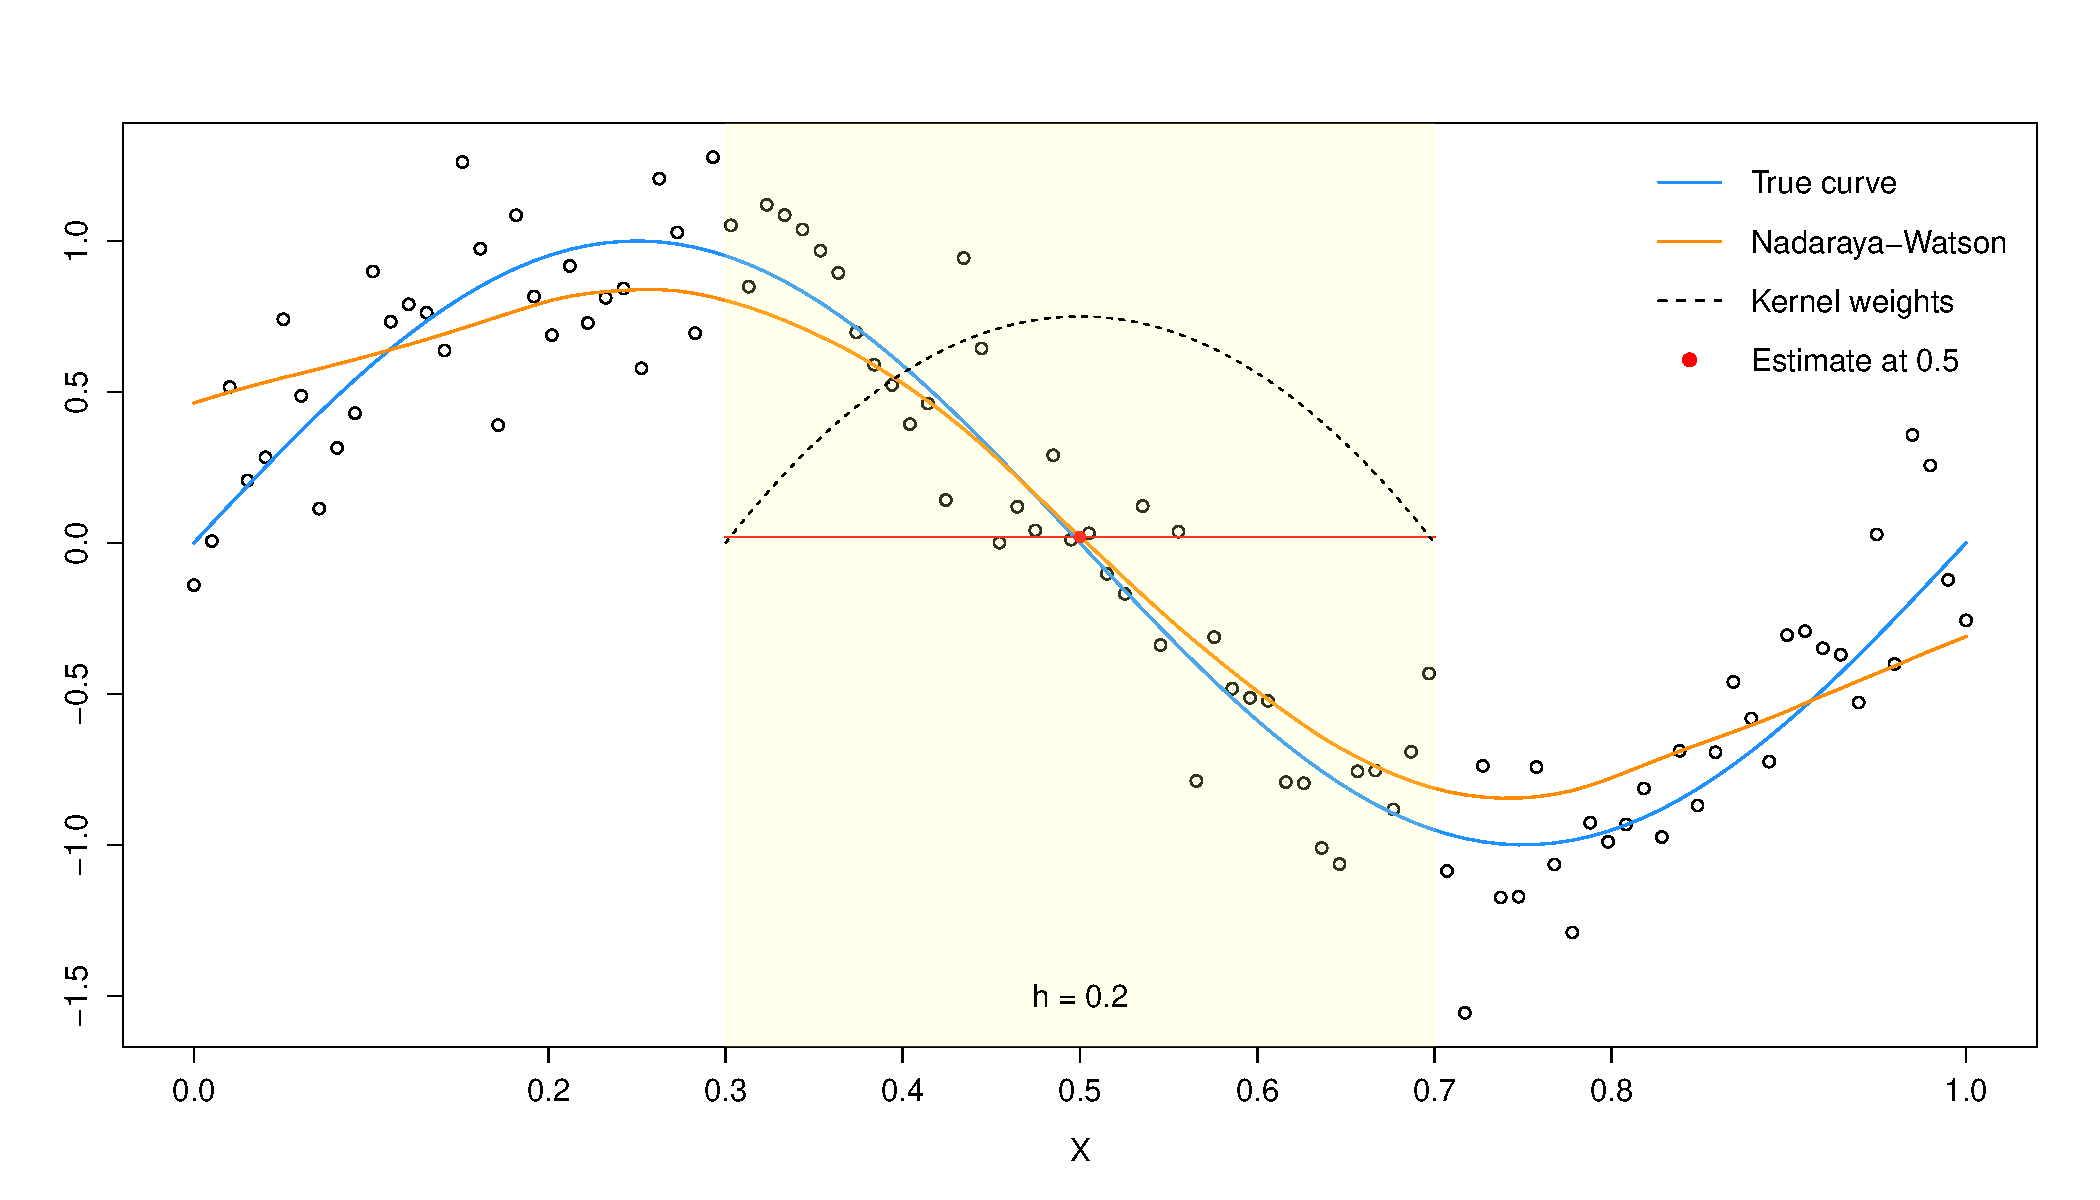
\includegraphics[trim=20 15 20 50, clip, width=\textwidth]{figure_01a.pdf}
		\caption{Estimation in the interior}
		\label{fig:nw_interior}
	\end{subfigure}

	\begin{subfigure}{0.75\textwidth}
		\centering
		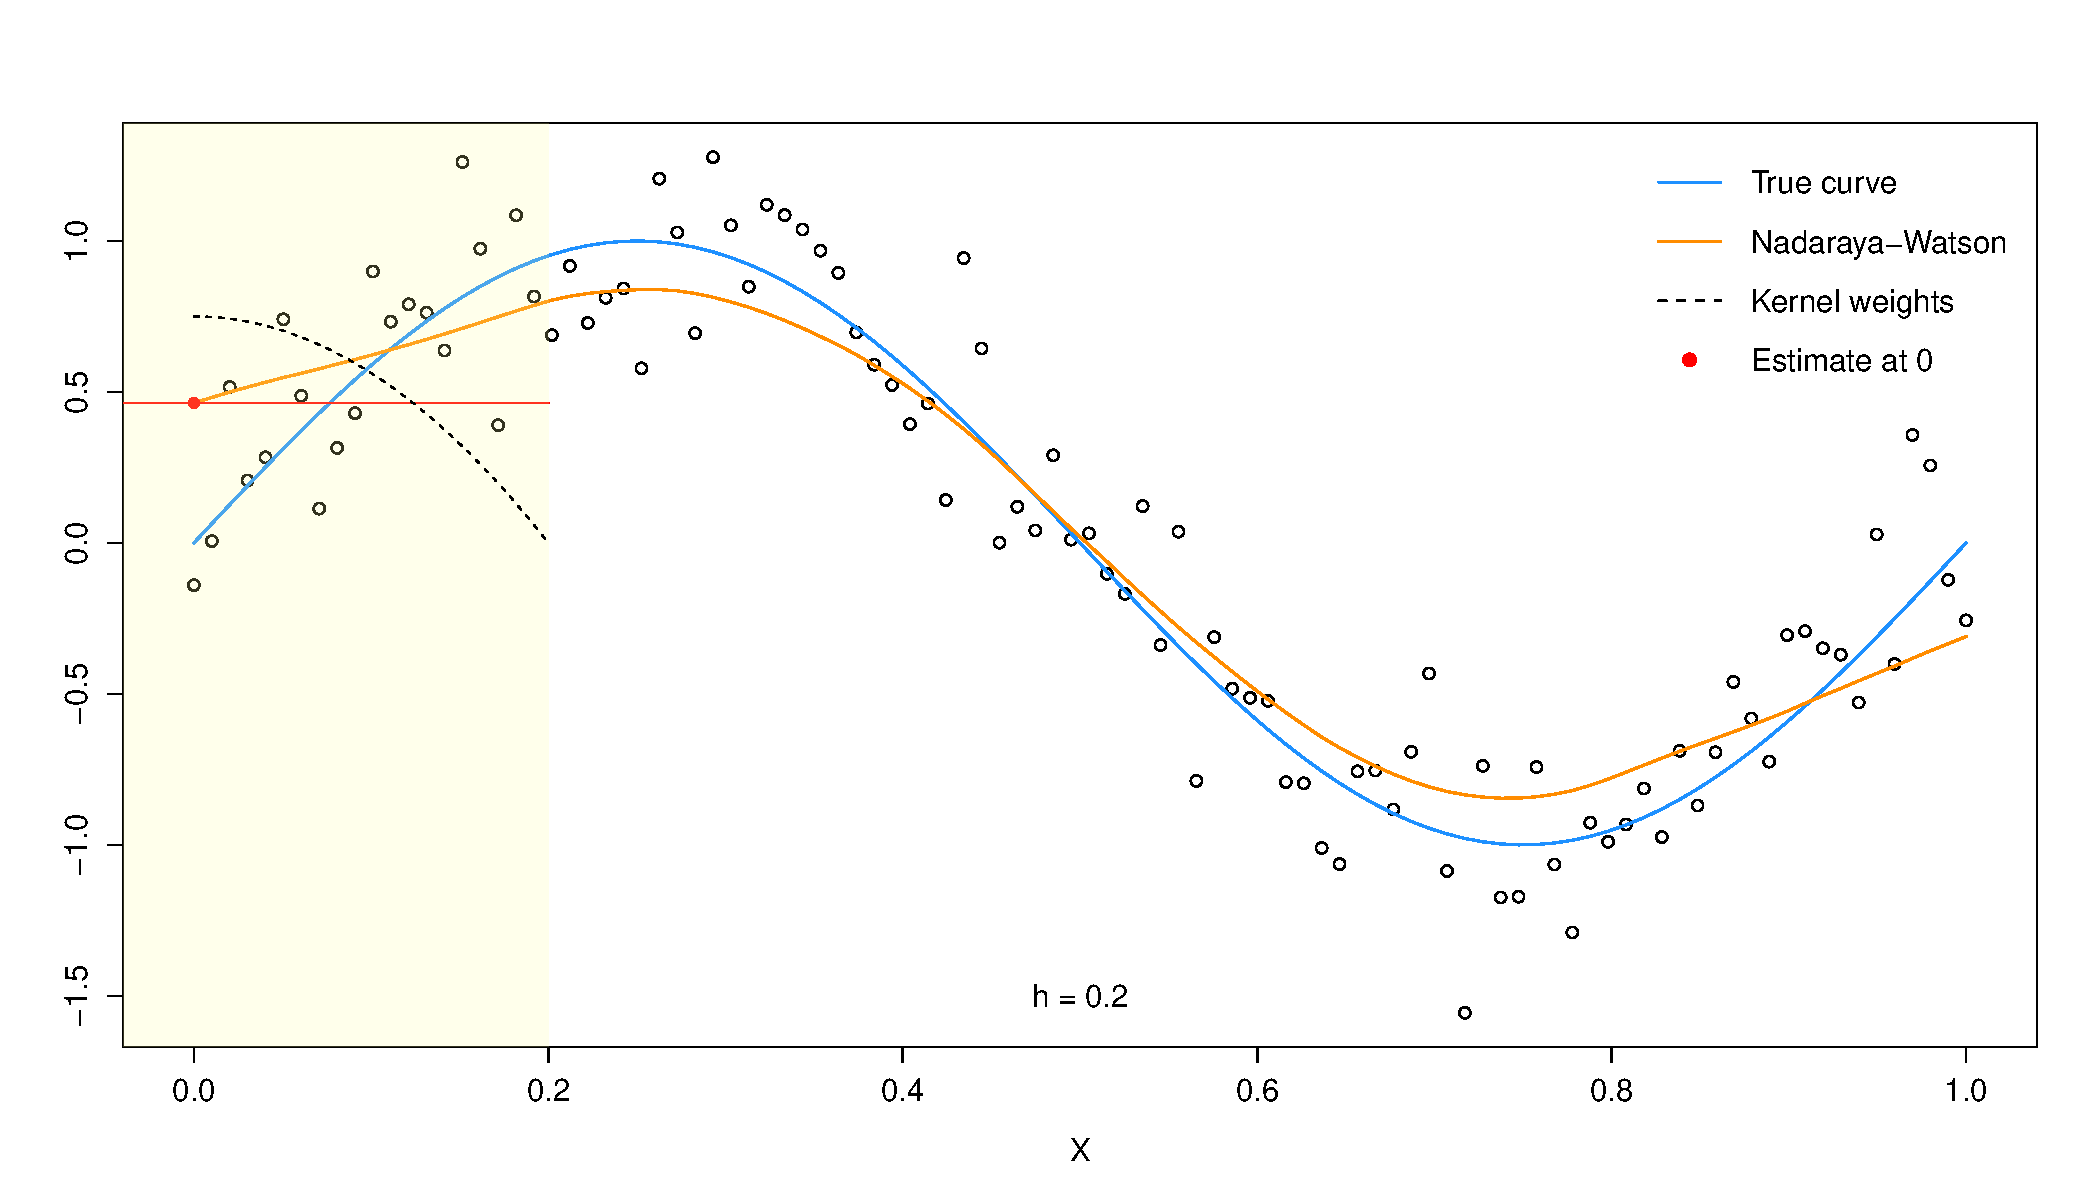
\includegraphics[trim=20 15 20 50, clip, width=\textwidth]{figure_01b.pdf}
		\caption{Estimation at the boundary}
		\label{fig:nw_boundary}
	\end{subfigure}
	\caption{Illustration of the estimation procedure underlying the Nadaraya-Watson estimator for 100 simulated observations (empty circles)}
	\label{fig:nw}
\end{figure}

Several methods have been proposed to overcome the boundary problem.
We focus on the two most relevant approaches.
First, the adjustment of the Nadaraya-Watson estimator by using special boundary kernels to asymptotically correct for the bias.
Second, local linear regression which locally fits a weighted regression line and is known to automatically correct the bias exactly to first order \parencite{Hastie_1993}.
The goal of this paper is then twofold.
Describing theoretically how both methods improve on the standard Nadaraya-Watson estimator.
And investigating the finite sample properties by means of Monte-Carlo simulations and a real-data application.

The Nadaraya-Watson estimator was independently proposed by \textcite{Nadaraya_1964} and \textcite{Watson_1964}.
The idea of locally weighted regression appeared first in \textcite{Stone_1977} and \textcite{Cleveland_1979}.
However, the favorable properties of the local linear estimator including boundary adaption were shown by
\textcite{Fan_1992} and \textcite{Fan_Gijbels_1992}.
\textcite{Ruppert_1994} extended the findings to the multidimensional setting.
\textcite{Gasser_1979} suggested the use of boundary kernels, but only provided ad hoc solutions.
Explicit formulas for polynomial boundary kernels are derived in \citeauthor{Müller_1991} (\citeyear{Müller_1991}, \citeyear{Müller_1993}) and \textcite{Müller_1994}.
\textcite{Gasser_1985} and \textcite{Granovsky_1991} also discuss boundary kernels.
Other methods to reduce the boundary bias include a generalized jackknife combination of two kernel estimators with different bandwidths
\parencite{Rice_1984, Kyung-Joon_1998}, as well as data reflection \parencite{Hall_1991}.

The remainder of the paper is structured as follows.
In the next section we formally introduce local linear regression and compare it to the Nadaraya-Watson estimator,
both theoretically and graphically.
Section~\ref{sec:boundary_kernels} discusses the idea and functioning of boundary kernels.
In Section~\ref{sec:simulation} we present a Monte-Carlo simulation study to compare the finite sample behavior of the methods.
An important application is given in Section~\ref{sec:application}:
the nonparametric estimation of causal effects in the regression discontinuity design (RDD).
Section~\ref{sec:conclusion} concludes.
The appendix contains proofs, information about kernels and additional figures and tables.
% TeX file "local_linear_regression"

% Research Module in Econometrics & Statistics 
% Prof. Dr. Liebl & Dr. Christopher Walsh
% Winter 2021/22, M.Sc. Economics, Bonn University
% Xingyu Tao, Xuan Li, Sven Jacobs


\section{Local linear regression} \label{sec:local_linear_regression}

We now first introduce local linear regression formally.
We then report the main results of the asymptotic analysis to compare both estimators.
A graphical approach illustrates the theoretical findings and builds intuition.

\subsection{Definition} \label{subsec:definition}

The Nadaraya-Watson estimator is also called a local constant estimator as it locally approximates the function $m$ as constant.
Hence, we obtain the estimator in \eqref{eq:nw} likewise from
\begin{equation}
	\hat{m}_{\NW}(x) = \argmin_{\beta_0} \sum_{i = 1}^{n} (Y_i - \beta_0)^2 K \left( \frac{X_i - x}{h} \right) \,.
\end{equation}
A natural extension is the weighted local fitting of a line with slope:
\begin{align}
	\hat{m}_{\LL}(x) &= \argmin_{\beta_0} \sum_{i = 1}^{n} (Y_i - \beta_0 - \beta_1(X_i - x))^2 K \left( \frac{X_i - x}{h} \right) \label{eq:ll} \\ 
	&= \sum_{i = 1}^{n} w(x, X_i, h) Y_i \,. \label{eq:linear_smoother}
\end{align}
We call $\hat{m}_{\LL}$ the local linear estimator.
From Equation~\eqref{eq:linear_smoother} we see that the estimator also belongs to the class of linear smoothers, i.e.\
it is a weighted average of the observed outcomes.
Since \eqref{eq:ll} is a standard weighted least squares problem, we obtain an explicit solution as (e.g.\ \cite[Section~5.2]{Wand_1995})
\begin{equation}
	\hat{m}_{\LL}(x) = \bm{e}_1^\top \left( \bm{X}_x^\top \bm{W}_x^{\vphantom{\top}} \bm{X}_x^{\vphantom{\top}} \right)^{-1} \bm{X}_x^\top \bm{W}_x^{\vphantom{\top}} \bm{Y} \,, 
\end{equation}
where invertibility of $\bm{X}_x^\top \bm{W}_x^{\vphantom{\top}} \bm{X}_x^{\vphantom{\top}}$ is assumed and 
\begin{equation}
	\bm{Y} = \begin{bmatrix} Y_1 \\ \vdots \\ Y_n \end{bmatrix},
	\bm{X}_x = \begin{bmatrix} 1 & X_1 - x \\ \vdots & \vdots \\ 1 & X_n - x  \end{bmatrix},
	\bm{W}_x = \diag \left\{ K \left( \frac{X_1 - x}{h} \right), \dots, K \left( \frac{X_n - x}{h} \right) \right\},
	\bm{e}_1 = \begin{bmatrix} 1 \\ 0 \\ \vdots \end{bmatrix} \,.
\end{equation}

If we apply the local linear estimator to the same data from Figure~\ref{fig:nw},
we achieve a much better estimation near the boundaries relative to the Nadaraya-Watson estimator.
This is depicted in Figure~\ref{fig:ll}.
To see how the bias is reduced, Figure~\ref{fig:ll_boundary} zooms in the estimation at the lower boundary $x = 0$.
Although half of the scaled kernel is not matched by any data, the estimated value is only slightly too high.
The reason is that the true curve can be well approximated by the fitted linear function on the interval $[0, 0.2]$. 
\begin{figure}
	\centering
	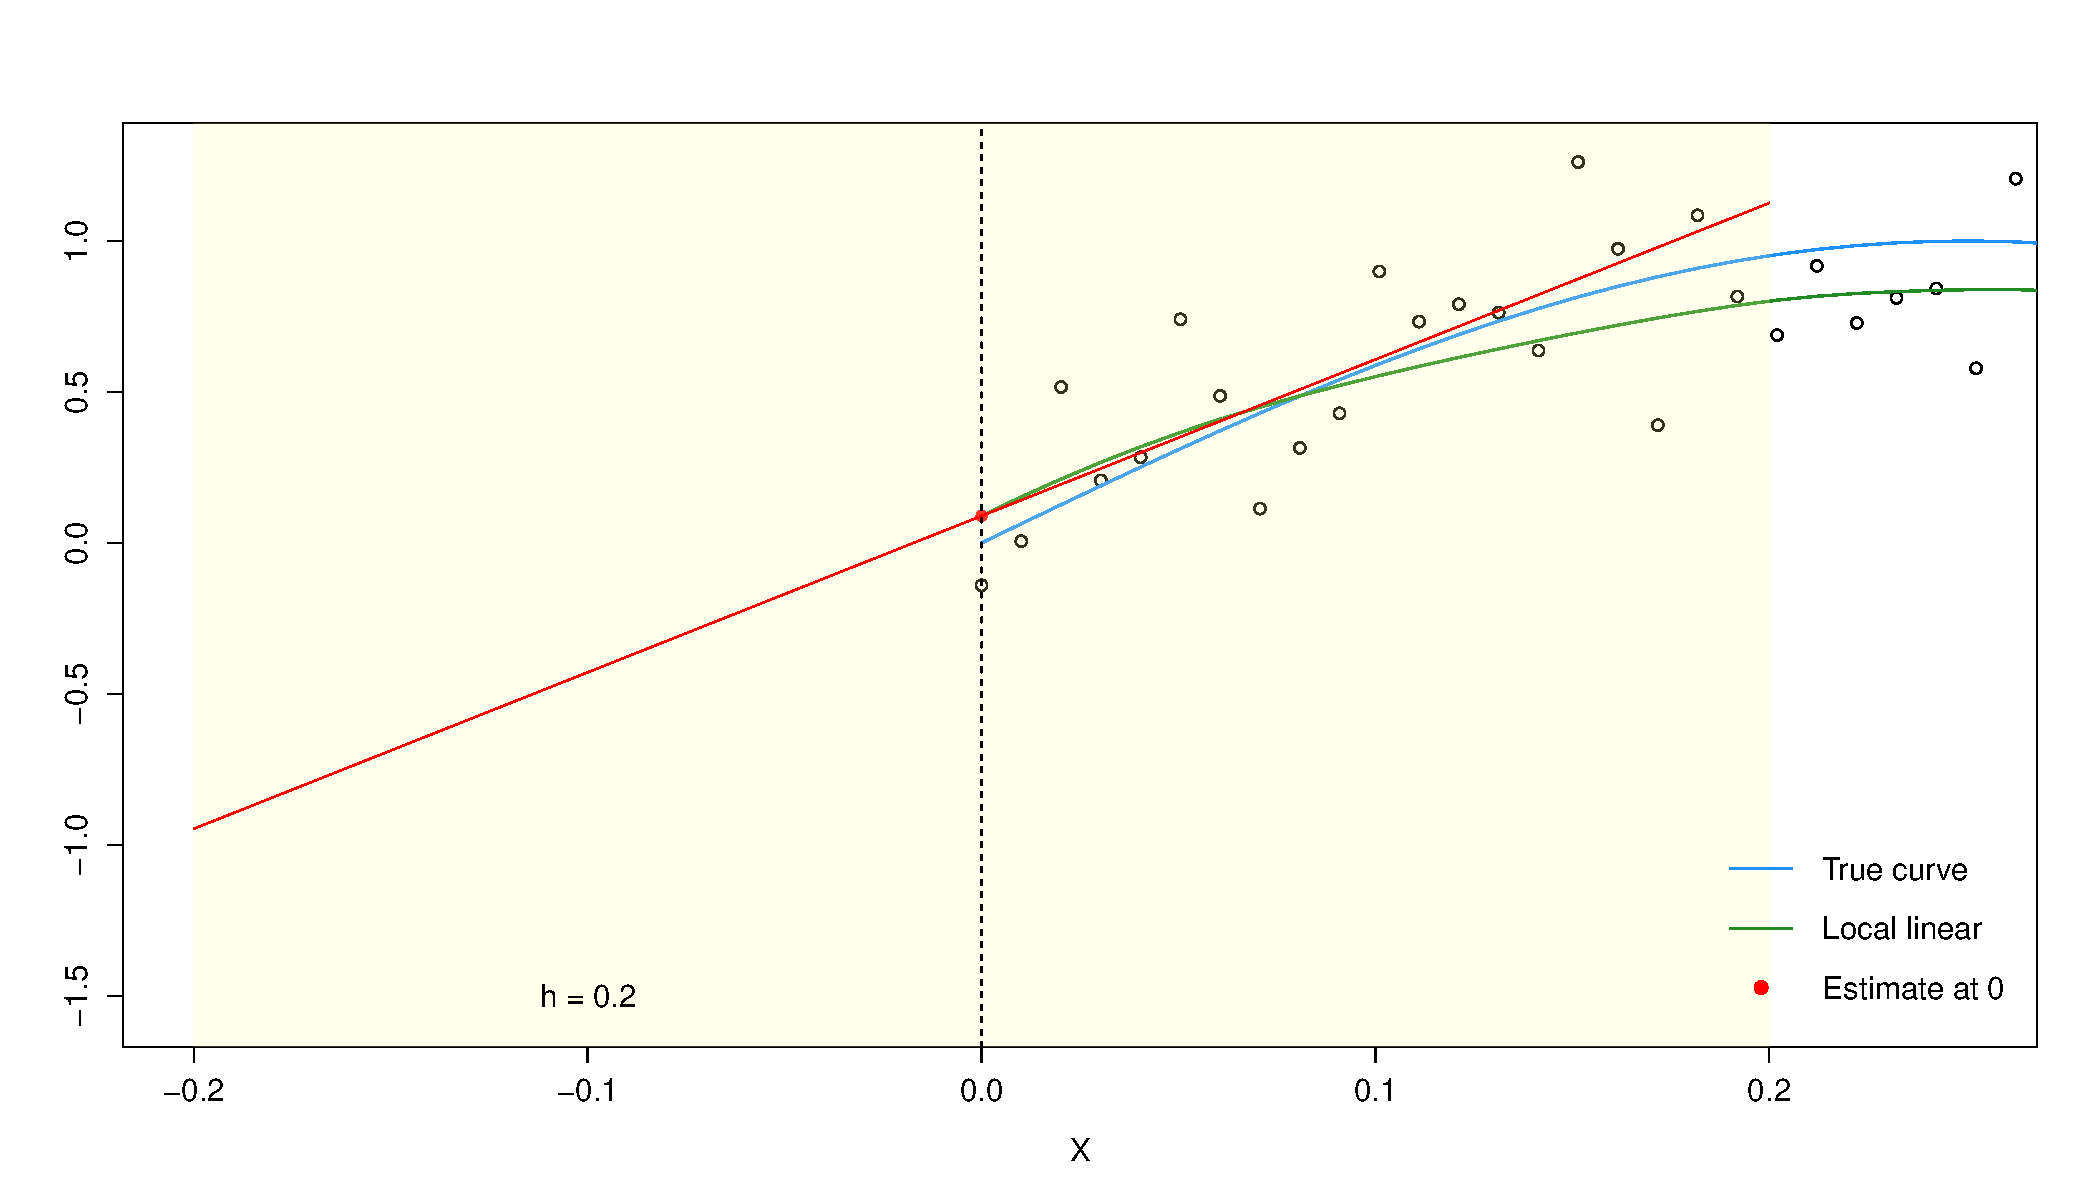
\includegraphics[trim=20 15 20 50, clip, width=0.75\textwidth]{figure_02.pdf}
	\caption{Illustration of the local linear estimate at the lower boundary $x = 0$.
			 Besides the point estimate also the locally fitted regression line is plotted.}
	\label{fig:ll_boundary}
\end{figure}

\begin{remark}
	Nadaraya-Watson ($p = 0$) and the local linear estimator ($p = 1$) are special cases of the local polynomial estimator,
	which locally fits a $p$-th degree polynomial to the data via least squares.
	To analyze the boundary correction provided by local polynomial regression, it suffices to look at the linear case.
\end{remark}

\subsection{Theoretical comparison} \label{subsec:theoretical_comparison}

The flexibility of nonparametric curve estimation makes a precise theoretical treatment for finite sample sizes complicated \parencite[15]{Härdle_1990}.
To gain the relevant insights into the performance of $\hat{m}_{\NW}$ and $\hat{m}_{\LL}$, we instead consider the asymptotic expressions,
i.e.\ the leading terms of bias and variance.
For the asymptotic analysis we rely on the following assumptions:
\begin{enumerate}[label=(A\arabic*), left=\parindent, itemsep=0pt]
	\item $m$ is twice continuously differentiable \label{A1}
	\item $f$ is continuously differentiable and $f(x)>0$
	\item $\sigma^2$ is continuous 
	\item $K$ is a symmetric and bounded pdf with $\kappa_2(K) \equiv \int u^2K(u) \diff u < \infty$ (finite variance) and $R(K) \equiv \int K(u)^2 \diff u < \infty$ (square integrability) \label{A4}
	\item $h \rightarrow 0, nh \rightarrow \infty$ as $n \rightarrow \infty$ \label{A5}
\end{enumerate}   
Assumption~\ref{A1} is a smoothness condition on the regression function needed for Taylor expansions.
We also assume certain smoothness of the design density $f$ and the conditional variance function $\sigma^2$.
The positive lower bound of $f$ is required because for the estimation the neighborhood of $x$ has to contain observations.
\ref{A4} states mild assumptions for the kernel function, which are satisfied for all kernels given in Table~\ref{tab:kernels}.
Lastly, to reduce bias the bandwidth $h$ has to get smaller yet the effective sample size $nh$ tends to infinity for the variance to vanish.

We start with the evaluation point $x$ being in the interior of the support of $f$.
Afterwards we move to the boundary.
The following theorem provides the core results for the estimation in the interior.
The proof for the Nadaraya-Watson estimator is presented in Appendix~\hyperref[appendix_1]{1}.
For the local linear estimator we refer the reader to \textcite[Section 3.7]{Fan_1996}.
\begin{theorem} \label{theorem_1}
	Let assumptions \ref{A1}--\ref{A5} be fulfilled and $x$ be in the interior of $\supp(f)$.
	Then, the conditional asymptotic bias is given by
	\begin{align}
		\ABias (\hat{m}_{\NW}(x) \,|\, \bm{X}) &= \frac{1}{2} \kappa_2(K) m''(x) h^2 + \kappa_2(K) \frac{m'(x)f'(x)}{f(x)} h^2 &=& \bigO(h^2) \,, \\
		\ABias (\hat{m}_{\LL}(x) \,|\, \bm{X}) &= \frac{1}{2} \kappa_2(K) m''(x) h^2 &=& \bigO(h^2) \,. \\
		\intertext{The conditional asymptotic variance is given by}
		\AVar (\hat{m}_{\NW}(x) \,|\, \bm{X}) &= \AVar (\hat{m}_{\LL}(x) \,|\, \bm{X}) = \frac{R(K) \sigma^2(x)}{f(x)} \frac{1}{nh} &=& \bigO\left( \frac{1}{nh} \right) \,.
	\end{align}
\end{theorem} 
Theorem~\ref{theorem_1} provides valuable insights into the properties of both estimators.
The asymptotic bias of $\hat{m}_{\LL}$ depends on the kernel constant $\kappa_2(K)$, the curvature of the unknown function $m$ and the squared bandwidth.
For a fixed bandwidth we obtain larger bias the curvier $m$.
Concavity leads to downward bias, convexity to upward bias.
This so-called smoothing bias (\enquote{trimming the hills and filling the valleys}) can also be seen in Figure~\ref{fig:ll}.
Overall, the order of $h^2$ means that for reduced bias in general a smaller bandwidth is required.
Looking next at the leading bias expression for the Nadaraya-Watson estimator, we notice the presence of a second term.
Due to its dependence on the design density the term is referred to as design bias.
Design bias is absent for uniform designs and more pronounced for stronger changes in $f$ and $m$.
Although the order of magnitude is the same, the interpretation is that $\hat{m}_{\LL}$ being design-adaptive \parencite{Fan_1992}
with simplified bias typically translates into reduced bias in practice \parencite[678]{Hansen_2022}.
Interestingly, the conditional asymptotic variance is the same for both estimators.
It is inversely proportional to the effective sample size, i.e.\ $\sim (nh)^{-1}$.

From Theorem~\ref{theorem_1} we can easily derive the asymptotically optimal local bandwidth minimizing the conditional asymptotic mean squared error (AMSE).
This yields $h_{\text{opt}}(x) \sim n^{-1/5}$ and $\AMSE_{\text{opt}}(x) \sim n^{-4/5}$.
An optimal global bandwidth is obtained as the minimizer of the density-weighted integrated AMSE (AMISE),
\begin{equation}
	h_{\text{opt}} \equiv \argmin_{h \,>\, 0} \int_{\supp(f)}^{} \AMSE(x) f(x) \diff x \,.
\end{equation} 
The solution for the Nadaraya-Watson and the local linear estimator, respectively, is given in the following theorem.
\begin{theorem} \label{theorem_2}
	The bandwidth minimizing the AMISE is given by
	\begin{align}
		h_{\textup{opt}}^{\LL}(n) &= \left\{ \frac{R(K) \int \sigma^2(x) \diff x}{\kappa_2(K)^2 \int (m''(x))^2 f(x) \diff x} \right\}^{1/5} \cdot n^{-1/5} \,, \\
		h_{\textup{opt}}^{\NW}(n) &= \left\{ \frac{R(K) \int \sigma^2(x) \diff x}{\kappa_2(K)^2 4 \mathlarger{\int} \left[ \frac{1}{2} m''(x) + \frac{m'(x) f'(x)}{f(x)} \right]^2 f(x) \diff x} \right\}^{1/5} \cdot n^{-1/5} \,.
	\end{align}
	With $h_{\textup{opt}} \sim n^{-1/5}$ it follows that $\AMISE_{\textup{opt}} \sim n^{-4/5}$. 
\end{theorem}     

In what follows we take $x$ to be exactly at the boundary, i.e.\ $x \in \{a, b\}$.
We draw on the same assumptions \ref{A1}--\ref{A5} as for the interior,
but now particularly require regarding \ref{A1} right-sided continuity at the lower boundary and left-sided continuity at the upper boundary.
In mathematical terms that is $\lim_{x \downarrow a} m''(x) = m''(a)$ and $\lim_{x \uparrow b} m''(x) = m''(b)$.
For the asymptotic theory of the local linear estimator at the boundary we define now truncated kernel moments, a projected kernel $\tilde{K}$ and its constants (see \cite[684]{Hansen_2022}):
\begin{align}
	\tilde{\kappa}_j(K) &\equiv \int_{0}^{\infty} u^jK(u) \diff u \,, \tilde{\tau}_j(K) \equiv \int_{0}^{\infty} u^jK(u)^2 \diff u \,, \\
	\tilde{K}(u) &\equiv \frac{\tilde{\kappa}_2 - \tilde{\kappa}_1 u}{\tilde{\kappa}_0^{\vphantom{2}} \tilde{\kappa}_2^{\vphantom{2}} - \tilde{\kappa}_1^2} K(u) \,, \\
	\tilde{\kappa}_2(\tilde{K}) &= \int_{0}^{\infty} u^2\tilde{K}(u) \diff u = \frac{\tilde{\kappa}_2^2 - \tilde{\kappa}_1^{\vphantom{2}}  \tilde{\kappa}_3^{\vphantom{2}}}{\tilde{\kappa}_0^{\vphantom{2}} \tilde{\kappa}_2^{\vphantom{2}} - \tilde{\kappa}_1^2} \,, \\
	\tilde{R}(\tilde{K}) &\equiv \int_{0}^{\infty} \tilde{K}(u)^2 \diff u = \frac{\tilde{\kappa}_2^2 \tilde{\tau}_0^{\vphantom{2}} - 2 \tilde{\kappa}_1^{\vphantom{2}} \tilde{\kappa}_2^{\vphantom{2}} \tilde{\tau}_1^{\vphantom{2}} + \tilde{\kappa}_1^2 \tilde{\tau}_2^{\vphantom{2}}}{(\tilde{\kappa}_0^{\vphantom{2}} \tilde{\kappa}_2^{\vphantom{2}} - \tilde{\kappa}_1^2)_{\vphantom{2}}^2} \,.
\end{align}

Theorem~\ref{theorem_3} reports the main results.
\begin{theorem} \label{theorem_3}
	Let assumptions \ref{A1}--\ref{A5} be fulfilled and $x \in \{a, b\}$. Then, the conditional asymptotic bias for $\hat{m}_{\NW}$ is given by
	\begin{align}
		\ABias (\hat{m}_{\NW}(a) \,|\, \bm{X}) &= 2 \int_{0}^{\infty} u K(u) \diff u \, m'(a) h &=& \bigO(h) \,, \\
		\ABias (\hat{m}_{\NW}(b) \,|\, \bm{X}) &= -2 \int_{0}^{\infty} u K(u) \diff u \, m'(b) h &=& \bigO(h) \,. \\
		\intertext{The conditional asymptotic bias and variance at $x = a$ for $\hat{m}_{\LL}$ is given by}
		\ABias (\hat{m}_{\LL}(a) \,|\, \bm{X}) &= \frac{1}{2} \tilde{\kappa}_2(\tilde{K}) m''(a) h^2 &=& \bigO(h^2) \,, \\
		\AVar (\hat{m}_{\LL}(a) \,|\, \bm{X}) &= \frac{\tilde{R}(\tilde{K}) \sigma^2(a)}{f(a)} \frac{1}{nh} &=& \bigO\left( \frac{1}{nh} \right) \,.
	\end{align}
\end{theorem}
For the local linear estimator see \textcite[Section 19.10]{Hansen_2022} and \textcite[Theorem 3.3]{Fan_1996}.
For the derivation of the asymptotic boundary bias of the Nadaraya-Watson estimator we follow the steps in the proof for interior points (Appendix~\hyperref[appendix_1]{1}).
However, since at the boundary half of the kernel is not contained in the support of $f$, the integral in \eqref{eq:appendix_1_03} is now over the region $[0, \infty)$.
As a consequence, the leading term is \eqref{eq:appendix_1_04}.

From Theorem~\ref{theorem_3} we see that the asymptotic bias and variance of $\hat{m}_{\LL}$ look very similar to the expressions from Theorem~\ref{theorem_1}.
Most importantly, the orders are unchanged.
What differs are the constants as they depend now on the projected kernel $\tilde{K}$.
In contrast, consulting the asymptotic bias of $\hat{m}_{\NW}$ at either boundary we notice the larger order of $h$ compared to $h^2$.
Because of this discrepancy between the bias order in the interior and at the boundary we say that the Nadaraya-Watson estimator exhibits a boundary bias problem.
The local linear estimator instead preserves the order.
Moreover, the equations show that if the regression function $m$ is positively sloped at the boundaries,
$\hat{m}_{\NW}$ will have upward bias at the lower boundary and downward bias at the upper boundary (see e.g.\ Figure~\ref{fig:nw}). 

For finite samples there is always a boundary region instead of just one or two boundary points.
If we assume that $\supp(K) = [-1, 1]$ and w.l.o.g.\ that $f$ is supported on the unit interval $[0, 1]$,
then the boundary region equals $[0, h) \cup (1-h, 1]$.
For $0 \leq \rho < 1$ we call $x = \rho h$ a left boundary point and $x = 1 - \rho h$ a right boundary point.
\textcite[Theorem~3.2]{Fan_1996} derived for an arbitrary boundary point qualitatively identical results as in Theorem~\ref{theorem_3},
including as a special case $x \in \{a, b\}$ being an exact boundary point.

It follows that the asymptotically optimal bandwidth near the boundary for the Nadaraya-Watson estimator is now $\bigO(n^{-1/3})$,
thus smaller bandwidths are required due to increased bias.
The optimal AMSE gets inflated to $\bigO(n^{-2/3})$ relative to $\bigO(n^{-4/5})$ in the interior.

So far our analysis has been of asymptotic nature.
However, we can show that the local linear estimator is exactly unbiased to first order, also in the boundary region.
To do so, we write the conditional expectation of either estimator as
\begin{align}
	\E [\hat{m}(x) \,|\, \bm{X}] &= \sum_{i = 1}^{n} w_i(x) m(X_i) \\
	&= m(x) \sum_{i = 1}^{n} w_i(x) + m'(x) \sum_{i = 1}^{n} w_i(x) (X_i - x) + R \,,
\end{align}
where in the second equality a Taylor expansion around $x$ is performed and $R$ contains higher-order terms.
The exact correction of the bias to first order by $\hat{m}_{\LL}$ follows immediately from the next theorem.
The proof is in Appendix~\hyperref[appendix_1]{1}. 
\begin{samepage}
	\begin{theorem} \label{theorem_4}
		Consider the estimation of the local linear estimator at some point $x$, i.e.\ $\hat{m}_{\LL}(x) = \sum_{i = 1}^{n} w_i(x) Y_i$.
		Then:
		\begin{align}
			\sum_{i = 1}^{n} w_i(x) &= 1 \,, \\
			\sum_{i = 1}^{n} w_i(x) (X_i - x) &= 0 \,.
		\end{align}
	\end{theorem}
\end{samepage}
If the true regression function is linear (as in Figure~\ref{fig:boundary_effects_linear}),
the local linear estimator will not have any estimation bias over the full design region.
For the Nadaraya-Watson estimator the term $\sum_{i = 1}^{n} w_i(x) (X_i - x)$ at the boundary is necessarily unequal to zero as the weights are nonnegative.

We briefly summarize the findings.
For the interior the order of the bias for both estimators is the same.
However, local linear regression has the favorable design-adaptivity property.
Near the boundary, the bias of the Nadaraya-Watson estimator is of larger order, whereas the local linear estimator preserves the order.
The latter is first-order unbiased.

\subsection{Graphical comparison}

By now we have shown mathematically that local linear regression fixes the boundary issue the Nadaraya-Watson estimator has.
To develop a deeper understanding for how the bias correction is achieved in practice, a graphical analysis is desirable.
An informative graphical device, based on the concept of an effective kernel, was proposed by \textcite{Hastie_1993}.
Since both estimators belong to the class of linear smoothers, they can be written as $\hat{m}(x)~=~\sum_{i = 1}^{n} w(x, X_i, h) Y_i$.
The effective kernel at an estimation point $x$ is then defined as the set of weights $\{w(x, X_i, h)\}_{i = 1}^n$,
i.e.\ the effective weights assigned to observations.
The idea is now to plot the effective kernel against the $X_i$'s.

\begin{figure}[t]
	\centering
	\begin{subfigure}{0.75\textwidth}
		\centering
		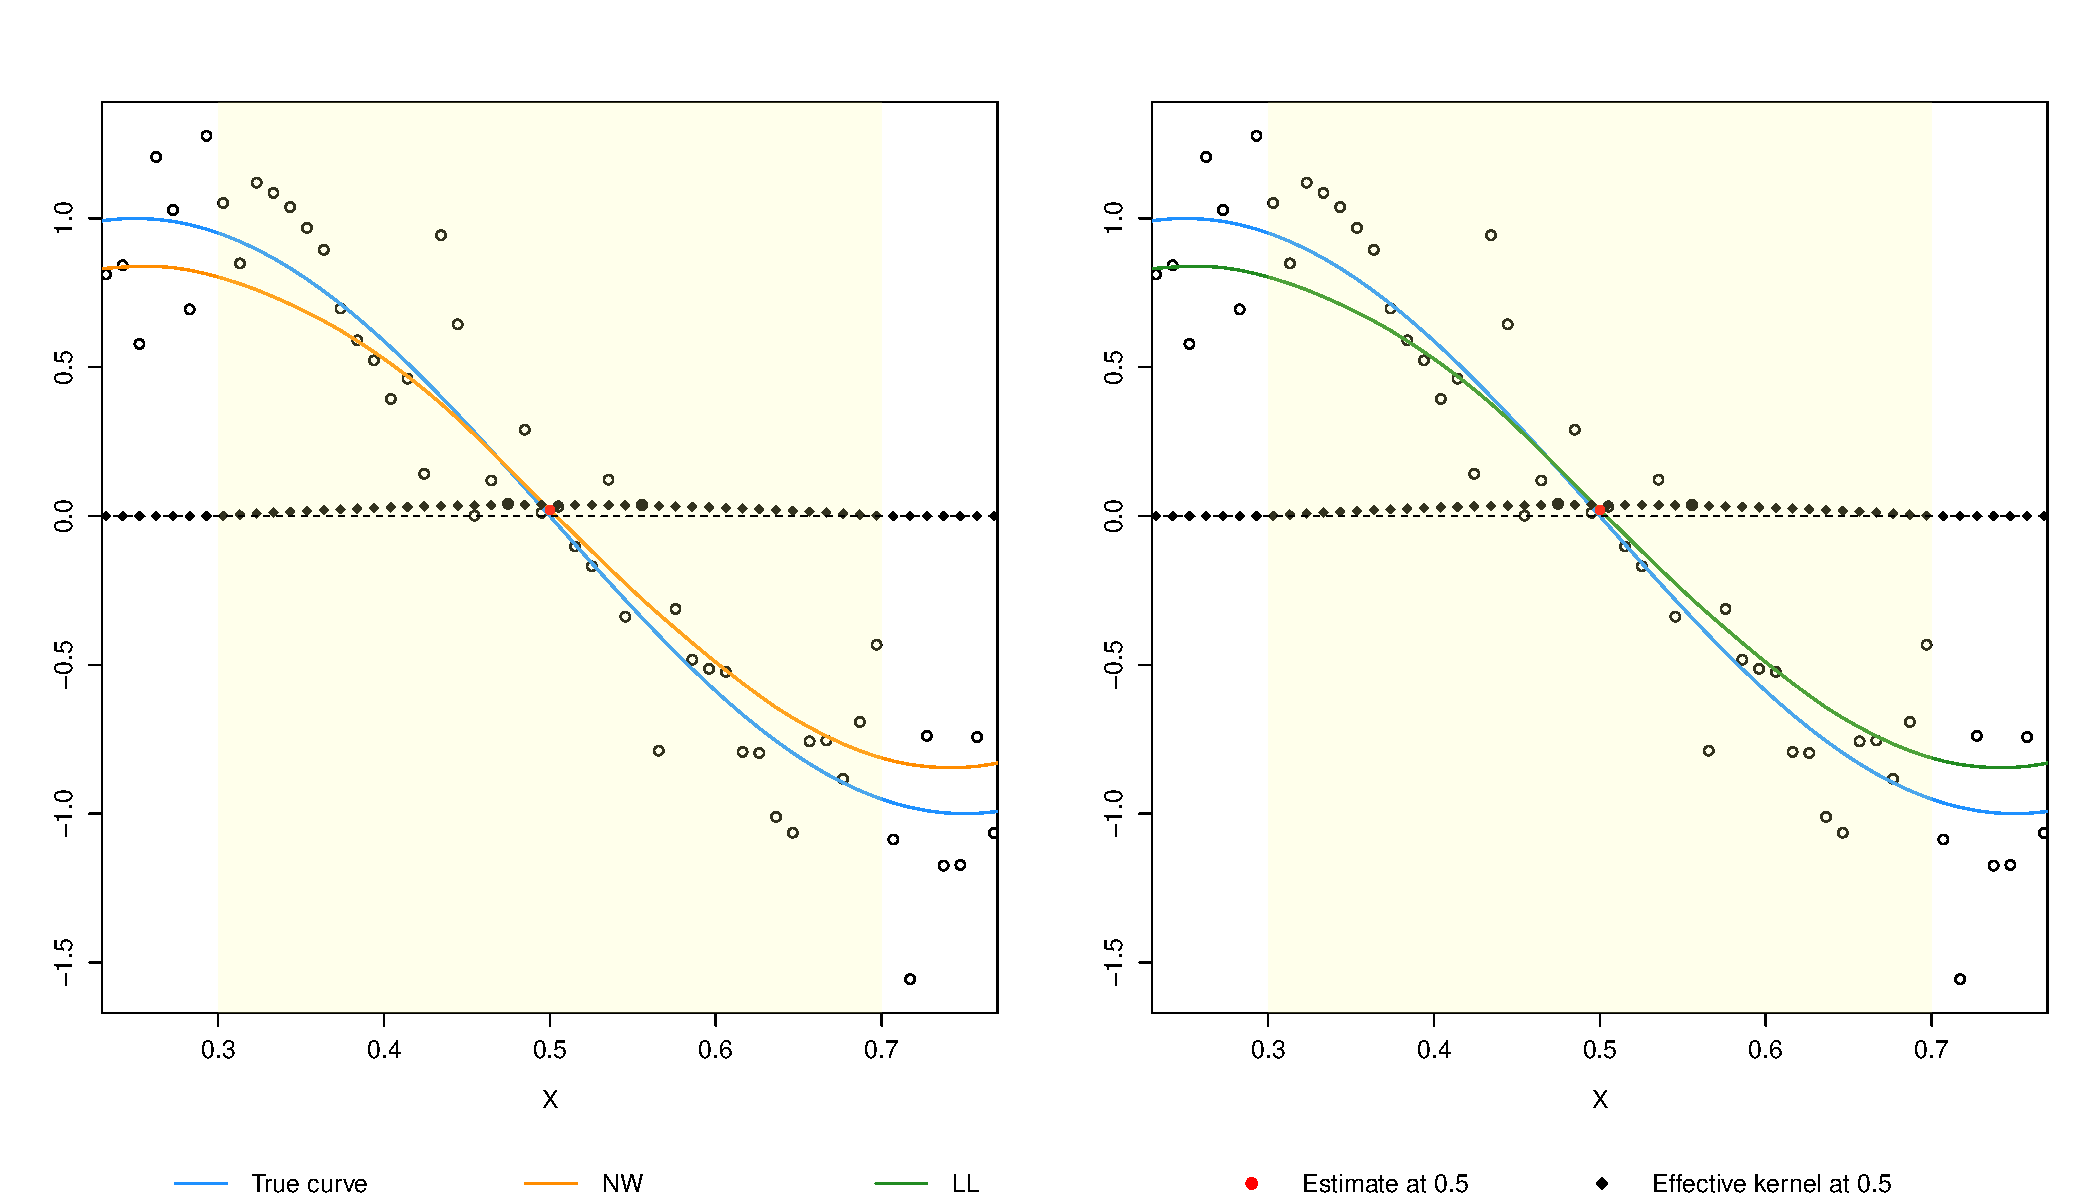
\includegraphics[trim=20 0 20 45, clip, width=\textwidth]{figure_03a.pdf}
		\caption{Effective kernel in the interior}
		\label{fig:effective_kernel_interior}
	\end{subfigure}
	
	\begin{subfigure}{0.75\textwidth}
		\centering
		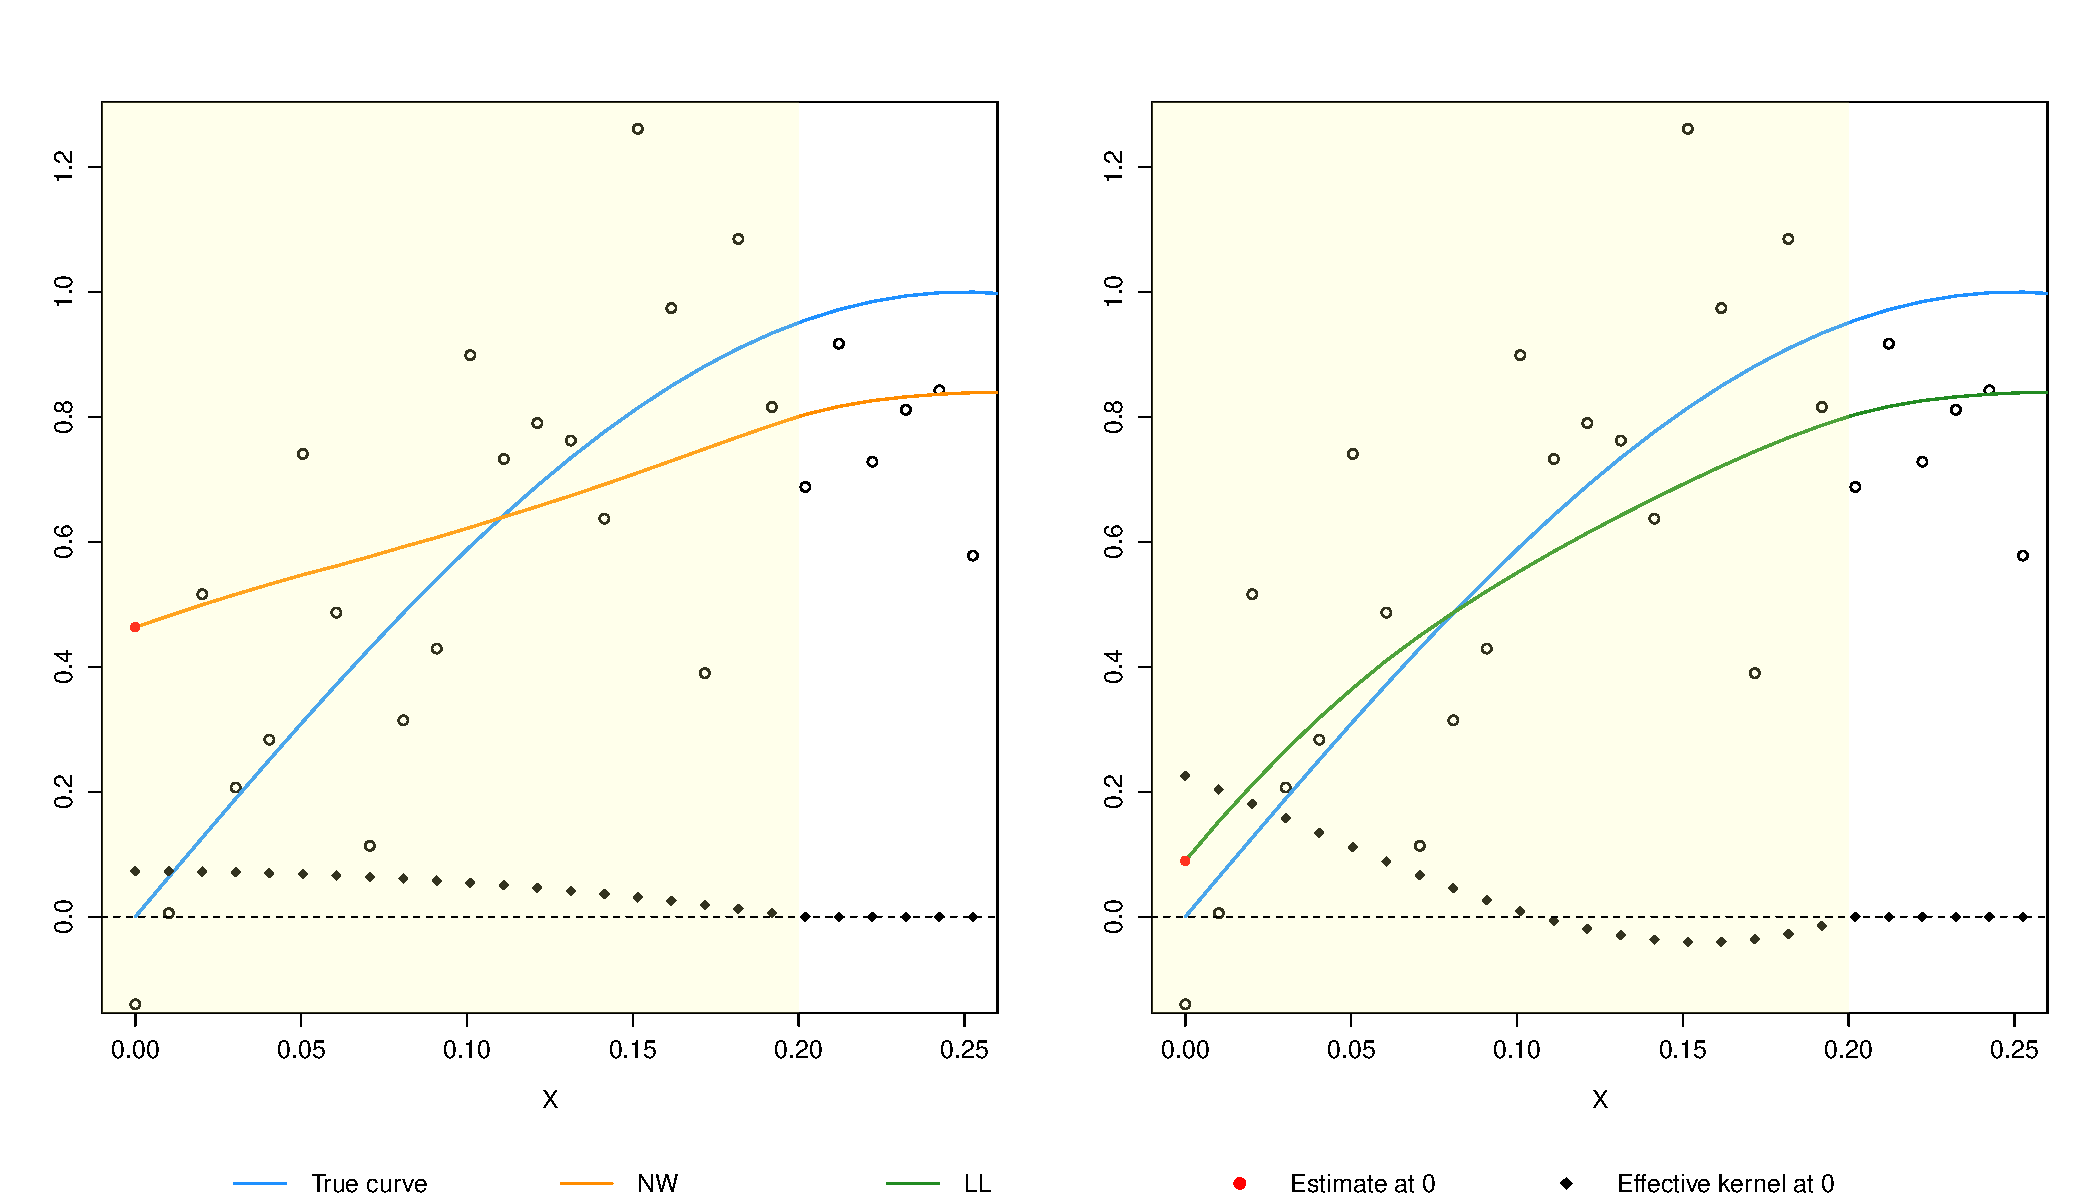
\includegraphics[trim=20 0 20 40, clip, width=\textwidth]{figure_03b.pdf}
		\caption{Effective kernel at the boundary}
		\label{fig:effective_kernel_boundary}
	\end{subfigure}
	\caption{Effective kernels for the Nadaraya-Watson estimator and the local linear estimator. The effective kernel is given by the filled squares.}
	\label{fig:effective_kernel}
\end{figure}

Figure~\ref{fig:effective_kernel_interior} shows the effective kernel for the Nadaraya-Watson and the local linear estimator, respectively, when estimating at the interior point $x = 0.5$.
The effective kernel is given by the black squares.
As these are literally the weights assigned to observations in the smoothing process, they sum up to one.
Only local data points in the yellow-shaded region receive positive weights, the more the closer $X_i$ is located to $x = 0.5$.
Overall, we do not see any difference between the two effective kernels.
The effectively assigned weights seem to be identical.

Next, we consider the estimation at the lower boundary $x = 0$.
This is presented in Figure~\ref{fig:effective_kernel_boundary}.
Once again, the large upward bias for the Nadaraya-Watson estimator is apparent.
Bias for the local linear estimator is much reduced.
For the Nadaraya-Watson estimator the effective kernel is just a rescaled version of the right side of the Epanechnikov kernel such that the added weights are one.
All weights in the estimation window are positive.
For local linear regression, in contrast, there are two effects visible leading to the improved boundary behavior.
First, $\hat{m}_{\LL}$ effectively assigns a much larger weight to observations in the immediate vicinity to $x = 0$.
Second, it puts a negative weight on the observations that are furthest away.
The negative weighting ensures that weights add to one and reverses the large bias observations far away from the boundary would contribute.
Figure~\ref{fig:effective_kernel_boundary} is a graphical illustration of Theorem~\ref{theorem_4}.
At boundary points the local linear estimator adapts automatically by deforming the effective kernel such that $\sum_{i = 1}^{n} w_i(x) (X_i - x) = 0$ holds.
The bias is removed to first order.
% TeX file "boundary_kernels"

% Research Module in Econometrics & Statistics 
% Prof. Dr. Liebl & Dr. Christopher Walsh
% Winter 2021/22, M.Sc. Economics, Bonn University
% Xingyu Tao, Xuan Li, Sven Jacobs


\section{Boundary kernels} \label{sec:boundary_kernels}

Before the boundary-adaptivity of local linear regression had been uncovered, the classical approach to compensate the boundary effects was to apply special boundary kernels for estimation in the boundary region.
The usage of such kernels provides an asymptotic correction for the boundary bias,
i.e.\ the order of the asymptotic bias will be $\bigO(h^2)$ near the boundary as in the interior.

To understand the definition of a boundary kernel, we recall that the $\bigO(h)$ boundary bias in Theorem~\ref{theorem_3} resulted
because the truncated kernel moment $\tilde{\kappa}_1(K) = \int_{0}^{\infty} u K(u) \diff u$ does not vanish.
The problem for an arbitrary boundary point can be stated in the boundary framework from Section~\ref{subsec:theoretical_comparison},
where $\supp(K) = [-1, 1]$, $\supp(f) = [0, 1]$ and the boundary region is $[0, h) \cup (1-h, 1]$.  
Then, for a left boundary point $\int_{-\rho}^{1} u K(u) \diff u \neq 0$ causes the worse order.
A boundary kernel is then an asymmetrically supported kernel that restores the original moment properties \parencite{Gasser_1979}. 
Thus, for $x = \rho h$ a left boundary kernel $K_{\text{l}}(u, \rho)$ satisfies for $\rho \in [0, 1]$
\begin{equation}
	\int_{-\rho}^{1} u^j K_{\text{l}}(u, \rho) \diff u = \begin{cases} 
		1 & j = 0 \\
		0 & j = 1 \\
		\neq 0 & j = 2 
	\end{cases} \,.
\end{equation}
Notice that the kernel shape changes with the relative location of $x$ to the boundary, expressed through the parameter $\rho$. 

\textcite[Table 1]{Müller_1991} derived a boundary kernel that can be seen as a continuation of the Epanechnikov kernel onto the boundary.
The left-sided kernel is given for $\rho \in [0, 1]$ by
\begin{align}
	K_{\text{E,\,l}}(u, \rho) = \begin{cases}
		6 (1-u) (\rho + u) \frac{1}{(1+\rho)^3} \left\{ 1 + 5\left( \frac{1-\rho}{1+\rho} \right)^2 - 10\frac{1-\rho}{(1+\rho)^2} u \right\} & \text{if } u \in [-\rho, 1] \\
		0 & \text{else}
	\end{cases} \,. 
\end{align}
The equivalent for the upper boundary is obtained by $K_{\text{E,\,r}}(u, \rho) = K_{\text{E,\,l}}(-u, \rho)$.
Figure~\ref{fig:epanechnikov_boundary} plots these kernels for selected values of $\rho$.
For the special case $\rho = 1$ the boundary kernel agrees with the interior kernel,
and estimation at the boundaries is included as $\rho = 0$.
The figure illustrates that the kernel shape differs the more (i.e.\ a larger portion of negative weights is assigned),
the closer the evaluation point $x$ is to the boundary.
The way how boundary kernels work in practice is the same as for the effective kernel of local linear regression at the boundary in Figure~\ref{fig:effective_kernel_boundary}.
In fact, theoretical results suggest that the local linear estimator implicitly induces a boundary kernel-type bias correction \parencite{Ruppert_1994}.
\begin{figure}
	\centering
	\begin{tikzpicture}
		\begin{axis}
			[
			grid, grid style={white}, 
			samples=1000, 
			domain=-1:1, 
			xlabel=$u$,
			ylabel={$K_{\text{E,\,l}}(u, \rho)$},
			legend entries={$\rho = 1$, $\rho = 0.5$, $\rho = 0$},
			legend style={draw=none, font=\footnotesize}, legend cell align={left}, legend pos={north west},
			width=0.45\textwidth
			]
			
			\addplot[black]
			expression {epa_right(-x, 1)};
			
			\addplot[black, dashed]
			expression {epa_right(-x, 0.5)};
			
			\addplot[black, dotted]
			expression {epa_right(-x, 0)};
		\end{axis}
	\end{tikzpicture}
	\qquad
	\begin{tikzpicture}
		\begin{axis}
			[
			grid, grid style={white}, 
			samples=1000, 
			domain=-1:1, 
			xlabel=$u$,
			ylabel={$K_{\text{E,\,r}}(u, \rho)$},
			legend entries={$\rho = 1$, $\rho = 0.5$, $\rho = 0$},
			legend style={draw=none, font=\footnotesize}, legend cell align={left},
			width=0.45\textwidth
			]
			
			\addplot[black]
			expression {epa_right(x, 1)};
			
			\addplot[black, dashed]
			expression {epa_right(x, 0.5)};
			
			\addplot[black, dotted]
			expression {epa_right(x, 0)};
		\end{axis}
	\end{tikzpicture}
	\caption{Left- and right-sided Epanechnikov boundary kernels for different values of $\rho$}
	\label{fig:epanechnikov_boundary}
\end{figure}

Applying the boundary-adjusted Nadaraya-Watson estimator with the Epanechnikov boundary kernels to the simulated data from Figure~\ref{fig:nw},
we find that the explicit adjustment corrects for a substantial amount of the original boundary bias (see Figure~\ref{fig:nw_boundary_adjusted}).
However, performance is slightly worse than the local linear fit.
Figure~\ref{fig:effective_kernel_nw_boundary} reveals why.
Since \textcite{Müller_1991} required continuity at the endpoints of the boundary kernels (\enquote{smooth optimum boundary kernels}),
the closest observations to $x = 0$ receive considerably less weight compared to the local linear estimator.
A class of boundary kernels with greater asymptotic efficiency at the cost of discontinuity is given in \textcite{Müller_1994}.

\begin{remark}
	Local bandwidth choice is now much more involved since for each $\rho$ a different bias-variance trade-off arises
	(e.g.\ \cite[Section 4]{Müller_1991}).
\end{remark}
% TeX file "simulation"

% Research Module in Econometrics & Statistics 
% Prof. Dr. Liebl & Dr. Christopher Walsh
% Winter 2021/22, M.Sc. Economics, Bonn University
% Xingyu Tao, Xuan Li, Sven Jacobs


\section{Simulation} \label{sec:simulation}

Our analysis of the estimators and their behavior near boundaries so far has been mainly based on asymptotic theory.
Thus, the correction of boundary kernels is only approximate for finite sample sizes.
For local linear regression we have shown the exact first-order bias correction, but the variability remains to be investigated.
To assess the finite sample properties of the estimators, we conduct a Monte-Carlo simulation study.
We first describe the set-up of the simulation.
Afterwards we present and discuss the results. 

\subsection{Set-up}

The kernel we are using is the Epanechnikov kernel.
Two reasons support this choice.
First, the kernel is asymptotically optimal for the estimation in the interior (see Appendix~\hyperref[appendix_2]{2}).
Second, its compact support on $[-1, 1]$ leads to faster computations and well-defined boundary regions.
The optimal kernel for the boundary region is the Triangular kernel \parencite{Cheng_1997}.
However, the efficiency loss of using the Epanechnikov kernel instead is negligible \parencite[684]{Hansen_2022}.
For the boundary-adjusted Nadaraya-Watson estimator we apply the Epanechnikov boundary kernels from Section~\ref{sec:boundary_kernels}.
As apparent from our theoretical analysis, the choice of the smoothing parameter $h$ is much more important.
Practical bandwidth selection is a broad topic on its own with several proposed procedures including, for example,
plug-in techniques and rules of thumb.
A popular approach, we use for the application in Section~\ref{sec:application}, is based on cross-validation.
The interested reader can find a detailed discussion of bandwidth selection in \textcite[Sections 3, 5.8]{Wand_1995}.
For the simulation we directly employ the asymptotically optimal global bandwidths from Theorem~\ref{theorem_2}.
We do not consider local selection due to the additional noise, its complexity for boundary points and complicated boundary regions that may arise.

Table~\ref{tab:simulation_overview} presents the six cases chosen for the simulation study.
We consider three regression functions whose graphs are shown in Figure~\ref{fig:simulation_functions}.
The function $m_1$ was used for simulating the data in the previous sections.
Function $m_2$ is a linear function with a peak in the interior, representing a linear boundary.
Function $m_3$ is similar to $m_2$, but the peak is shifted to lie approximately at the left boundary zero, representing a structured boundary.
In general, the regressor $X$ is taken to be uniformly distributed on $[0, 1]$ and
the error to be homoscedastic with distribution $\epsilon \sim \mathcal{N}(0, 0.25^2)$.
To study the performance of the estimators in a lower and higher signal-to-noise environment,
we modify the error variance when estimating $m_1$.
Lastly, we also look at the case of a non-uniform design as expressed by the design density $f_{\ast}$.
Figure~\ref{fig:clustered_design_density} reveals that $f_{\ast}$ reflects a clustered design, where fewer observations occur closer to the boundaries.

\renewcommand{\arraystretch}{1.5}	
\begin{table} \small
	\centering
	\captionabove{Selected cases for the simulation study}
	\label{tab:simulation_overview}
	\begin{tabular}{l l c l}  
		\toprule
		Regression function $m$ & Design & $\sigma^2(X)$ & Feature \\
		\midrule
		$m_1(x) = \sin(2 \pi x)$ 							  				 & $X \sim \mathcal{U}(0, 1)$ & $0.25^2$ & Example from Figure~\ref{fig:nw} \\
		$m_1(x) = \sin(2 \pi x)$ 							   				 & $X \sim \mathcal{U}(0, 1)$ & $0.10^2$ & High signal-to-noise ratio \\
		$m_1(x) = \sin(2 \pi x)$ 							   				 & $X \sim \mathcal{U}(0, 1)$ & $0.50^2$ & Low signal-to-noise ratio \\
		$m_1(x) = \sin(2 \pi x)$ 							                 & $X \sim f_{\ast}$ 		  & $0.25^2$ & Clustered (non-uniform) design \\
		$m_2(x) = 2 -2x + 2 \exp \left\{ \frac{-(x - 0.5)^2}{0.01} \right\}$ & $X \sim \mathcal{U}(0, 1)$ & $0.25^2$ & Linear function, peak in interior \\
		$m_3(x) = 2 -2x + 2 \exp \left\{ \frac{-(x - 0)^2}{0.01} \right\}$   & $X \sim \mathcal{U}(0, 1)$ & $0.25^2$ & Linear function, peak at boundary \\           
		\bottomrule \addlinespace[1ex]
		\multicolumn{4}{l}{$f_{\ast}(x) = 3 \cdot \{ 5/12 - (x - 0.5)^2 \}_{[0, \, 1]}$} 
	\end{tabular}	
\end{table}
\renewcommand{\arraystretch}{1.0}

The goodness-of-fit measure to evaluate the boundary behavior is the mean integrated squared error (MISE) over the left boundary region of the Nadaraya-Watson estimator,
i.e.\ $[0, h_{\text{opt}}^{\NW}(n))$.
For each of the six simulation cases we compute for seven representative sample sizes (from $n = 50$ to $n = 5000$) the percentage changes in the boundary MISE of the local linear estimator
and the boundary-adjusted Nadaraya-Watson estimator to the standard Nadaraya-Watson estimator.
Figure~\ref{fig:simulation_set-up} illustrates the main part of the procedure for the function $m_1$ and a sample size of $n = 100$.
The optimal bandwidth in this example is $h_{\text{opt}}^{\NW}(100) = 0.104$, giving the yellow-shaded boundary region.
The dark yellow area then reflects the integrated error of the unadjusted Nadaraya-Watson fit over the region of interest for a single random sample.
To obtain the MISE, we proceed as follows.
For $B$ Monte-Carlo repetitions with $n$ random observations,
we use numerical integration to calculate the integrated squared error (ISE).
Then, the expectation is approximated according to the law of large numbers by taking the average of the $B$ many ISE realizations:
\begin{equation}
	\MISE(n; \hat{m}) \approx \frac{1}{B} \sum_{j = 1}^{B} \ISE_j(n; \hat{m}) \,.
\end{equation}
The number of Monte-Carlo iterations equals $B = 10000$ for the first four sample sizes including $n = 500$ and $B = 1000$ otherwise.

The simulation study was conducted in $\mathsf{R}$. \nocite{R_2021}
All methods are self-implemented.

\subsection{Results and discussion}

We begin with the first case from Table~\ref{tab:simulation_overview}.
The simulation results are displayed in Table~\ref{tab:simulation_results_m_1}a.
We discuss this baseline case in greater detail since it reveals certain general patterns.
We note that for uniform designs (here on [0, 1]) the bandwidths for the Nadaraya-Watson (NW) and the local linear (LL) estimator coincide,
because then the asymptotic bias is the same (design bias is absent).
We see that the bandwidth gets smaller yet the effective sample size grows (from $nh = 5.95$ to $nh = 235$).
For $n = 50$ the left boundary region is about one tenth of the observation interval.
For this sample size the NW estimator performs best at the left boundary.
The MISE of the LL estimator is 789\% larger, for the boundary-adjusted NW estimator it is even 1578\%.
However, one should keep in mind that the absolute numbers are quite small.
From the sample size $n = 100$, LL regression yields a lower MISE, and the improvement increases with the sample size.
For $n = 5000$ the reduction amounts to 89\%.
In contrast, the application of boundary kernels pays off starting from a sample size of $n = 1000$.
Thereafter, the percentage reduction approaches the numbers achieved by LL regression.
For $n = 5000$ the reduction in the MISE amounts to 85\%.
Besides, we notice one unusual result for the adjusted NW estimator, namely a jump in the MISE change for 250 observations.
In summary, the simulated values show three developments.
First, LL regression quickly leads to improved boundary behavior which grows steadily.
Second, for smaller sample sizes the explicit boundary adjustment performs worse but achieves a lower MISE for larger samples.
And third, the larger the sample size the smaller is the gap between the two boundary correction methods.    

\begin{table}
	\centering
	\captionabove{Simulated percentage changes in the boundary MISE.
				  The regression function is $m_1$ (Subtables (a)--(d) correspond to cases one to four from Table~\ref{tab:simulation_overview}).}
	\label{tab:simulation_results_m_1}
	\begin{tabular}{r r r r}
		\toprule
		\multirow{2}[1]{*}{$n$} & \multirow{2}[1]{*}{Boundary region: $[0, h_{\text{opt}}^{\NW}(n))$} & \multicolumn{2}{c}{Change in MISE to NW [\%]} \\
		\cmidrule(lr){3-4} 
		& & Local linear & NW boundary-adjusted \\
		\midrule \addlinespace[2ex]
		\multicolumn{4}{c}{(a) $X \sim \mathcal{U}(0, 1)$, $\sigma^2(X) = 0.25^2$} \\[1ex]
		50   & [0, 0.119) & 	 789.29 & 	  1578.07 \\
		100  & [0, 0.104) & \redm 41.90 & 	  1143.28 \\
		250  & [0, 0.086) & \redm 65.13 & 	  1982.67 \\
		500  & [0, 0.075) & \redm 72.98 &   	14.92 \\
		1000 & [0, 0.065) & \redm 77.75 & \redm 65.84 \\
		2500 & [0, 0.055) & \redm 84.48 & \redm 77.33 \\
		5000 & [0, 0.047) & \redm 89.10 & \redm 84.82 \\[1ex]
		\multicolumn{4}{c}{(b) $X \sim \mathcal{U}(0, 1)$, $\sigma^2(X) = 0.10^2$} \\[1ex]
		50   & [0, 0.083) & 	1108.76 & 	  2782.59 \\
		100  & [0, 0.072) &  	 829.54 & 	  2651.04 \\
		250  & [0, 0.060) & \redm 82.21 & 	   660.80 \\
		500  & [0, 0.052) & \redm 86.45 & 	  1404.17 \\
		1000 & [0, 0.045) & \redm 88.91 & \redm 71.03 \\
		2500 & [0, 0.038) & \redm 92.47 & \redm 85.65 \\
		5000 & [0, 0.033) & \redm 94.70 & \redm 90.46 \\[1ex]
		\multicolumn{4}{c}{(c) $X \sim \mathcal{U}(0, 1)$, $\sigma^2(X) = 0.50^2$} \\[1ex]
		50   & [0, 0.157) & 	  29.02 & 	  1211.54 \\
		100  & [0, 0.137) & \redm 21.12 & 	  1713.05 \\
		250  & [0, 0.114) & \redm 43.81 & 	   160.39 \\
		500  & [0, 0.099) & \redm 55.65 & \redm 19.68 \\
		1000 & [0, 0.086) & \redm 63.34 & \redm 51.37 \\
		2500 & [0, 0.072) & \redm 73.52 & \redm 64.01 \\
		5000 & [0, 0.063) & \redm 81.22 & \redm 76.20 \\[1ex]
		\multicolumn{4}{c}{(d) $X \sim f_{\ast}$, $\sigma^2(X) = 0.25^2$} \\[1ex]
		50   & [0, 0.114) & 	1710.42 & 	   768.81 \\
		100  & [0, 0.099) &    78059.16 & 	  5265.00 \\
		250  & [0, 0.082) & \redm 47.65 & 	  1194.28 \\
		500  & [0, 0.072) & \redm 59.66 & 	   569.77 \\
		1000 & [0, 0.062) & \redm 66.92 & 	   169.63 \\
		2500 & [0, 0.052) & \redm 75.70 & \redm 43.91 \\
		5000 & [0, 0.045) & \redm 81.78 & \redm 69.66 \\
		\bottomrule
	\end{tabular}	
\end{table}

The reason for the better boundary performance of the LL estimator for all sample sizes except $n = 50$ is its first-order unbiasedness.
Since over the boundary regions the function $m_1$ can be well approximated by a linear function (see Figure~\ref{fig:ll_boundary}),
LL regression accomplishes a substantial bias reduction compared to the NW estimator.
However, the procedure is more variable than Nadaraya-Watson.
For $n = 50$ we only have on average six (noisy) observations in the boundary region.
Then, fitting locally a regression line is unstable and the variability dominates.
In fact, if we decrease the error variance while keeping the bandwidth fixed, at some point the bias reduction results in a smaller error for $n = 50$.
It can also be shown mathematically that the asymptotic variance of the LL estimator tends to become inflated near the boundary \parencite[Section 5.5]{Wand_1995}.
The results for the boundary-adjusted NW estimator illustrate the fact that the boundary correction is only asymptotically valid (as discussed in Section~\ref{sec:boundary_kernels}).
A sufficient amount of data ($n = 1000$) is necessary until the bias modification works in the considered simulation case.
The more data is effectively available, the less will the results between the LL estimator and the adjusted NW estimator differ
because we know from the theoretical treatment that both possess $\bigO(h^2)$ boundary bias.
Asymptotically the methods perform equivalently.
Lastly, to investigate the MISE increase for $n = 250$ when using boundary kernels,
we modified the noise level while everything else remained unchanged.
Only for a very small error variance close to the degenerate case, we observed a monotonically decreasing error.
Further investigation is necessary to understand this finding, also because the same behavior occurs for other set-ups. 

Next, starting from the baseline case we alter the variance of the homoscedastic error.
Table~\ref{tab:simulation_results_m_1}b reports the results for a smaller variance of $\sigma^2 = 0.1^2$ and Table~\ref{tab:simulation_results_m_1}c for $\sigma^2 = 0.5^2$, a variance four times the initial value $0.25^2$.
We might infer from the discussion of the baseline case that, for instance,
LL regression will achieve better (worse) results for a higher (lower) signal-to-noise ratio.
However, a change in the (conditional) error variance leads to a new bias-variance trade-off, and thus to different optimal bandwidths.
According to Theorem~\ref{theorem_2} a decrease (increase) of $\sigma^2$ results in smaller (larger) bandwidths.
Indeed, looking at Table~\ref{tab:simulation_results_m_1}b we notice a larger MISE over the boundary region for the LL estimator also for $n = 100$.
But for a sample size of $n = 250$ and beyond, the MISE reduction is stronger than in Table~\ref{tab:simulation_results_m_1}a
(e.g.\ 17 percentage points for $n = 250$).
A similar behavior is obtained for the boundary-adjusted NW estimator.

The reason for the increased MISE of both approaches relative to the NW estimator for smaller samples is the reduced effective sample size.
Even though observations falling into the boundary region are now on average more informative,
the lower number causing a higher estimation variability gives a relative advantage to NW.
If more data is effectively available, we see the dominating bias reduction effect.
Overall, Table~\ref{tab:simulation_results_m_1}b shows the same patterns as before (for the same reasons as before).
LL regression exhibits for all sample sizes better boundary behavior than the adjusted NW estimator,
the latter requires more data to achieve a MISE reduction, but the difference between both methods vanishes asymptotically.

For the increased error variance $\sigma^2 = 0.5^2$ we obtain opposite results to the lowest variance case,
which is in line with the explanation just given.
Compared to the baseline case bandwidths are now 32\% larger.
The MISE of LL regression for $n = 50$ is only 29\% larger, and the explicit boundary adjustment is already advantageous for 500 observations.
But the magnitude of the reductions is smaller compared to the two higher signal-to-noise cases.
For example, the reduction of the LL estimator for $\sigma^2 = 0.5^2$ and $n = 5000$ is with 81\% about the same as for $\sigma^2 = 0.1^2$ and only $n = 250$.
Estimation near the boundary is based on more observations, but these are less reliable due to a four-time higher error variance.

An interesting question is how the finite sample properties of the estimators depend on the design,
i.e.\ how the observations of the regressor are distributed.
To analyze the dependence, we again consider the baseline case and modify the design from being uniform to being clustered.
Compared to the uniform design the clustered design density $f_{\ast}$ from Table~\ref{tab:simulation_overview} gradually shifts half of the probability mass to the center (see Figure~\ref{fig:clustered_design_density}).
Hence, in practice the closer a region is located to the boundaries, the fewer observations will occur.
We point out that the non-uniform design induces a different bandwidth for the NW and the LL estimator (the latter ones are 4\% larger).
The design switch has essentially no effect on the size of the boundary region.
When comparing the MISE changes to those for the uniform design,
LL regression and overall also adjusted NW perform inferior.
For $n = 100$ the LL estimator shows a strong increase in the MISE, yet from a sample size of $n = 250$ reductions are achieved.
For the adjusted NW estimator instead $n = 2500$ observations are needed to get an improvement.

The worse boundary behavior (and the jump at $n = 100$) for the clustered design appears due to fewer observations near the boundary compared to the uniformly distributed regressor.
Moreover, the results indicate the fact that LL regression is design-adaptive while the adjusted NW method is not.
Boundary kernels are adaptive to the boundary but not to non-uniform designs near the boundary.
See \textcite{Hastie_1993} for a graphical illustration.

After discussing the results for $m_1$, we now examine the case of a linear conditional expectation function with a bump in the interior.
Figure~\ref{fig:m_2} displays the graph of $m_2$ and the simulation results are given in Table~\ref{tab:simulation_results_m_2}.
First, we notice the considerably smaller bandwidths compared to before.
Even for the smallest sample size $n = 50$, the bandwidth is already $h = 0.066$.
Second, although over the boundary regions the function $m_2$ is exactly linear,
neither boundary correction method leads to improved estimation, also not for the largest sample size.

The small bandwidths result from the peak in the interior of the observation interval (avoidance of excessive smoothing bias).
Then, LL regression has relatively high MISE values despite having zero estimation bias.
The functional form of $m_2$ was chosen to illustrate two points.
The NW estimator has an advantage in contexts where estimation variance is the decisive component,
i.e.\ when the effective sample size is small or estimation bias is low because the regression function is rather flat.
And, when evaluating boundary behavior it is important to choose a suitable research design.
If the smoothing parameter is selected globally, the boundary analysis may be dominated by an interior feature like a peak in our example.
To focus on boundary estimation without interference, we could either truncate the interval [0, 1] to exclude the peak
or try to incorporate local bandwidth choice (e.g.\ \cite{Fan_Gijbels_1992}).    

\begin{table}
	\centering
	\captionabove{Simulated percentage changes in the boundary MISE.
				  The regression function is $m_2$ (case five from Table~\ref{tab:simulation_overview}).}
	\label{tab:simulation_results_m_2}
	\begin{tabular}{r r r r}
		\toprule
		\multirow{2}[1]{*}{$n$} & \multirow{2}[1]{*}{Boundary region: $[0, h_{\text{opt}}^{\NW}(n))$} & \multicolumn{2}{c}{Change in MISE to NW [\%]} \\
		\cmidrule(lr){3-4}
		& & Local linear & NW boundary-adjusted \\
		\midrule
		50   & [0, 0.066) &   15953.93 &   989.86 \\
		100  & [0, 0.057) & 1040283.95 &   724.15 \\
		250  & [0, 0.048) & 	 86.23 & 17438.86 \\
		500  & [0, 0.042) & 	 65.39 &   293.78 \\
		1000 & [0, 0.036) & 	 54.40 &   114.32 \\
		2500 & [0, 0.030) & 	 42.89 &    74.65 \\
		5000 & [0, 0.026) & 	 33.27 &    66.51 \\
		\bottomrule
	\end{tabular}	
\end{table}

In the final simulation case the regression function $m_3$ is similar to $m_2$, but the peak is shifted to the left boundary (Figure~\ref{fig:m_3}).
Consequently, as can be seen from Table~\ref{tab:simulation_results_m_3} the boundary regions are somewhat larger.
Qualitatively the results are now again similar to the ones for the function $m_1$.
For the smallest (effective) sample sizes LL regression is worse, but then quickly improves on NW in a constant manner
(the lower reduction for $n = 1000$ is an artifact of the fewer Monte-Carlo repetitions).
Regarding the adjusted NW estimator it takes longer (until $n = 1000$) to pay off.
When the boundary region contains at least a few observations ($nh = 250 \cdot 0.055 \approx 14$) the bias reduction achieved by LL regression takes over.
Due to the strong negative slope of $m_3$ in the boundary regions, NW has substantial downward bias.
In contrast, by modeling slopes LL regression is able to capture this structured boundary.
The asymptotic adjustment of boundary kernels instead is visible not until 1000 observations.

\begin{table}
	\centering
	\captionabove{Simulated percentage changes in the boundary MISE.
				  The regression function is $m_3$ (case six from Table~\ref{tab:simulation_overview}).}
	\label{tab:simulation_results_m_3}
	\begin{tabular}{r r r r}
		\toprule
		\multirow{2}[1]{*}{$n$} & \multirow{2}[1]{*}{Boundary region: $[0, h_{\text{opt}}^{\NW}(n))$} & \multicolumn{2}{c}{Change in MISE to NW [\%]} \\
		\cmidrule(lr){3-4}
		& & Local linear & NW boundary-adjusted \\
		\midrule
		50   & [0, 0.076) & 	 999.26 & 	 76196.73 \\
		100  & [0, 0.066) &    41922.93 & 	  5420.96 \\
		250  & [0, 0.055) & \redm 63.17 & 	   356.63 \\
		500  & [0, 0.048) & \redm 65.57 & 	   343.59 \\
		1000 & [0, 0.042) & \redm 64.64 & \redm 39.99 \\
		2500 & [0, 0.035) & \redm 66.81 & \redm 56.64 \\
		5000 & [0, 0.030) & \redm 69.30 & \redm 63.45 \\
		\bottomrule
	\end{tabular}	
\end{table}

We briefly summarize the simulation findings.
The LL estimator performs better than the adjusted NW estimator, particularly for small sample sizes and non-uniform designs.
Only for samples as large as 5000 or more the methods are equivalent.
When effective sample sizes are small and also when the regression function near the boundary is rather flat (estimation bias is negligible) NW is favorable.
When there is some structure, i.e.\ curvature, near the boundary and the effective sample size is roughly not smaller than $nh = 15$, then the LL estimator is beneficial.
% TeX file "application"

% Research Module in Econometrics & Statistics 
% Prof. Dr. Liebl & Dr. Christopher Walsh
% Winter 2021/22, M.Sc. Economics, Bonn University
% Xingyu Tao, Xuan Li, Sven Jacobs


\section{Application} \label{sec:application}

To showcase the practical use of the boundary correction methods,
we consider the nonparametric estimation of treatment effects in the regression discontinuity design (RDD).
RDD is a popular quasi-experimental research design to identify a causal effect as a jump of an outcome variable
at a known threshold of a so-called assignment variable.
This threshold constitutes a boundary.
When measuring the size of the discontinuity, i.e.\ the causal effect in a valid RDD,
boundary effects may severely bias the estimate and inference.
RDD was first applied by \textcite{Thistlethwaite_1960}.
\textcite{Hahn_2001} were the first to suggest local linear regression to estimate the conditional expectation function
at the threshold to avoid boundary bias.
Also see \textcite{Porter_2003}.
\textcite{Imbens_2012} investigated bandwidth choice specifically for RDD. 

In a widely-cited study \textcite{Lee_2008} applied RDD to analyze the causal effect of party incumbency on reelection probabilities in U.S. House elections.
Figure~\ref{fig:application_overview} shows the Democrats' probability of winning a seat in the U.S. House of Representatives in the next election against the Democratic vote share minus the vote share of the strongest opponent (almost always the Republicans).
Each data point is an average of the indicator variable for winning election $t+1$ for each interval, which is 0.005 wide.
To the left of the zero-threshold the Democratic nominee lost election t;
to the right, the Democratic party won.
We can see a smooth relationship between the two variables (higher reelection probability for a higher vote share),
except for the threshold at zero which decides about victory or defeat.
\textcite{Lee_2008} interprets the large discontinuity as the true electoral incumbency advantage
as he argues that due to the inherent uncertainty in the exact vote share, winning a close election is \enquote{as good as random}.
Then, districts where the Democrats just barely lost constitute a valid counterfactual for districts where the Democrats just barely won and became incumbent (receiving treatment).

The task is now to estimate the size of the discontinuity.
Figure~\ref{fig:application_fits} displays the fit of each method (NW, LL regression, boundary-adjusted NW) for each side of the threshold.
To select the bandwidths (we allow the degree of smoothing to differ for each side) we use leave-one-out cross-validation (LOOCV).
That is, the bandwidth that minimizes the sum of squared prediction errors:
\begin{align}
	h_{\text{\tiny CV}} &\equiv \argmin_{h \,>\, 0} \CV(h) \,, \text{where} \\
	\CV(h) &\equiv \frac{1}{n} \sum_{i = 1}^{n} (Y_i - \hat{m}_{-i}(X_i, h))^2 \equiv \frac{1}{n} \sum_{i = 1}^{n} \tilde{\epsilon}_i^2 \,.
\end{align}  
One can show that $h_{\text{\tiny CV}}$ is essentially an unbiased estimator of $h_{\text{\tiny MISE}}$ \parencite[Theorem~19.7]{Hansen_2022}.
The solution has to be obtained numerically, which can cause problems.
The function $\CV(h)$ can have multiple local minima (Figures~\ref{fig:application_left_nw}, \ref{fig:application_right_ll})
and the solution can be unbounded such that $h_{\text{\tiny CV}} = \infty$ (Figure~\ref{fig:application_left_ll}).
From the Figures~\ref{fig:application_left} and \ref{fig:application_right} we see that the cross-validated bandwidths are larger for the left side and for the LL estimator.  

\begin{figure}
	\centering
	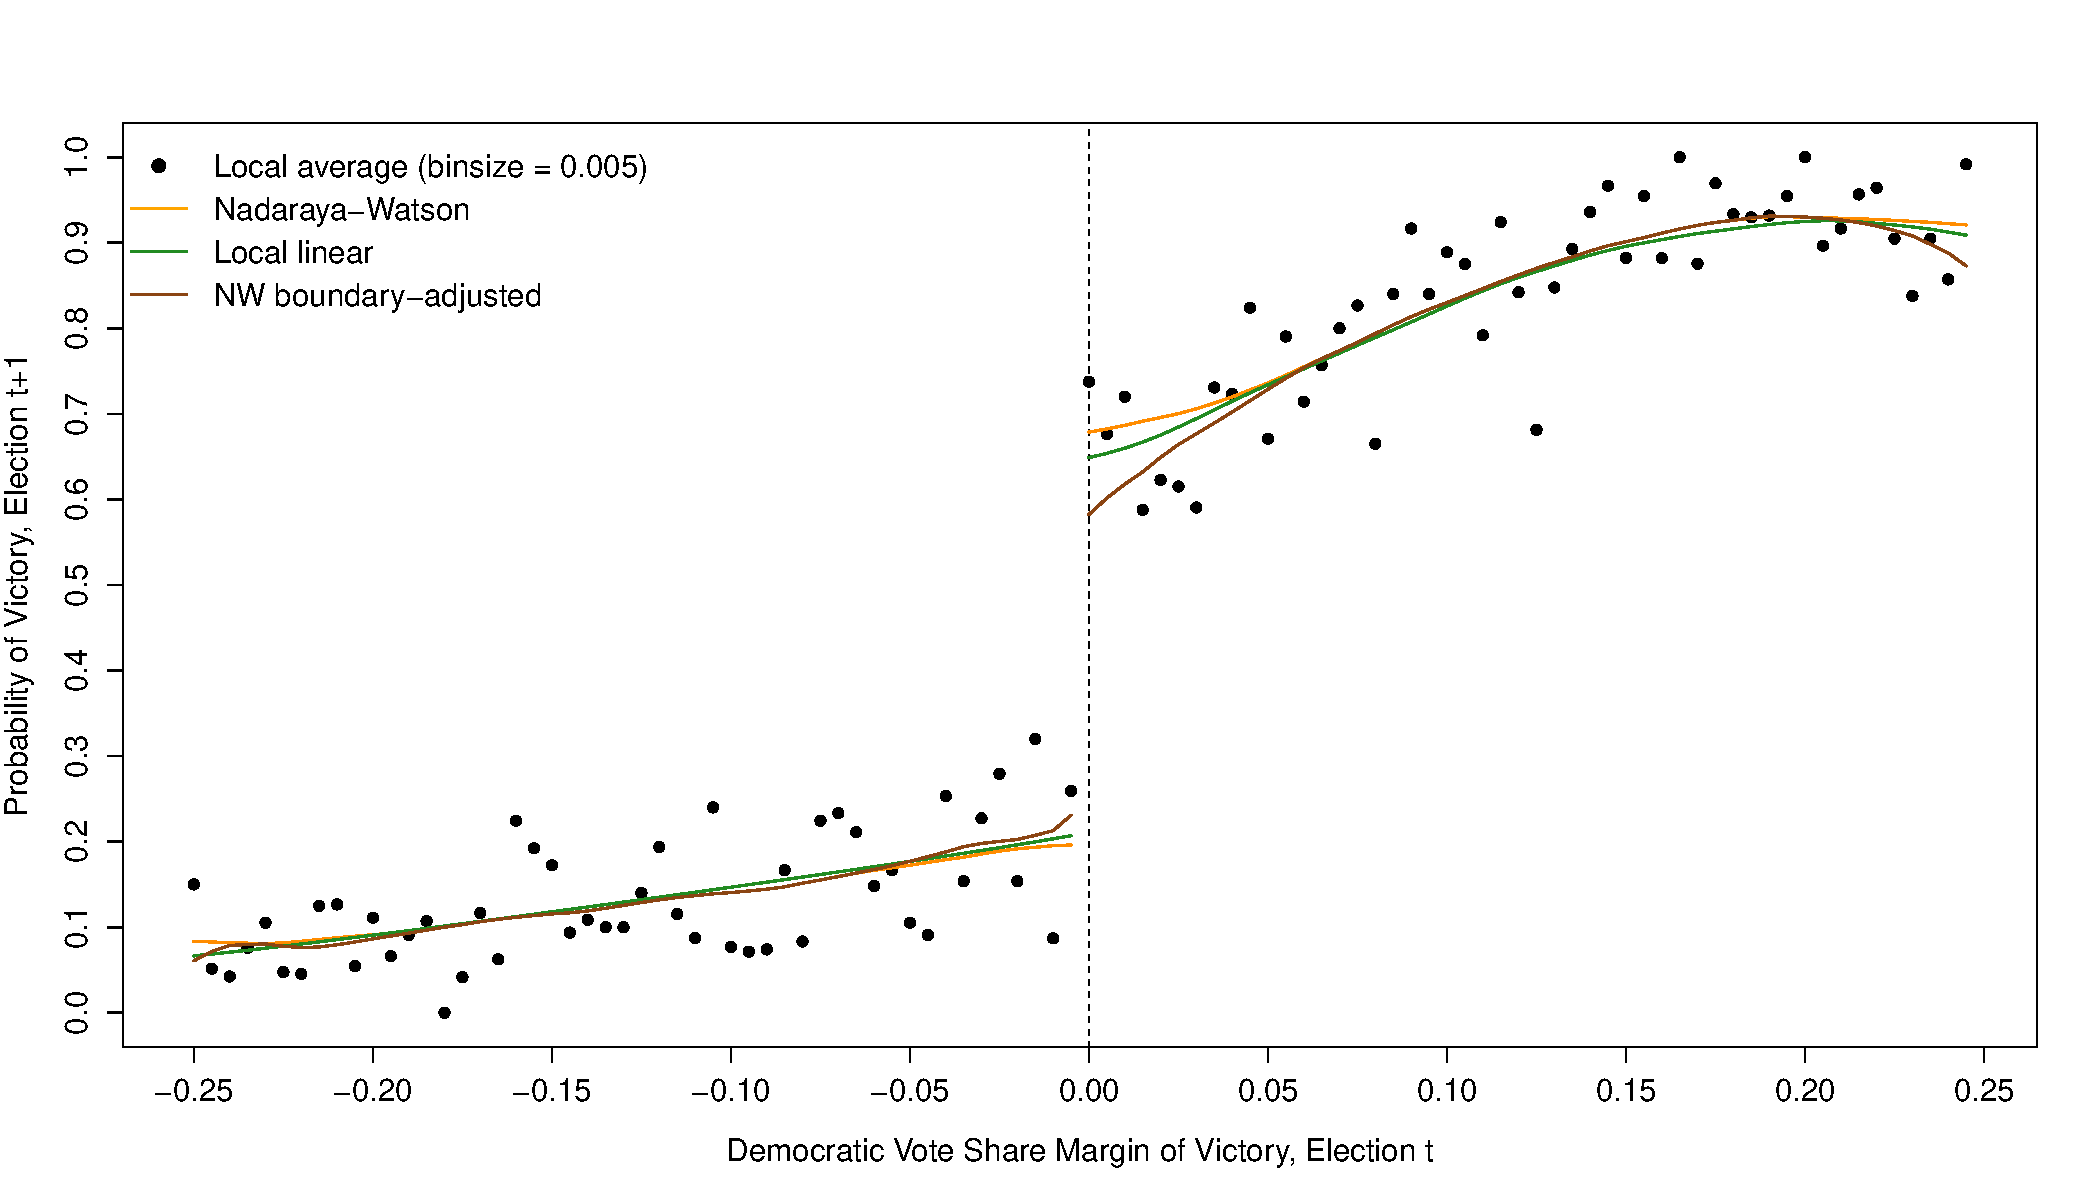
\includegraphics[trim=0 15 20 50, clip, width=0.75\textwidth]{figure_05.pdf}
	\caption{Democrats' probability of victory in election $t+1$, by margin of victory in election $t$.
			 Estimates of NW, LL regression and adjusted NW with cross-validated bandwidths.}
	\label{fig:application_fits}
\end{figure}

The estimates to the left side of the threshold look very similar.
However, since LL regression coincides with the global OLS fit (infinite bandwidth) the estimate is more stable yet captures the same structure.
In contrast, on the right side the estimates differ considerably near the boundary.
It is apparent that the NW estimate suffers from boundary bias as described in Section~\ref{sec:local_linear_regression}.
The explicit boundary adjustment results in a much smaller boundary estimate.
The curve resembles the parametric logit fit of \textcite[Fig.\ 5a]{Lee_2008}.
LL regression also leads to a smaller discontinuity estimate, but the correction is less strong.
Besides, the estimate is less wavy.
The figure illustrates the need for boundary correction.
Just looking at the right side to the threshold, NW suggests a ten percentage points greater incumbency advantage compared to adjusted NW;
and a more than three percentage points greater advantage compared to the LL estimator.
Based on Figure~\ref{fig:application_fits}, the simulation results and its simplicity we pick the LL estimator for further discussion.

We can construct asymptotic confidence intervals to assess precision.
Theorem~\ref{theorem_5} states that the local polynomial estimator is asymptotically normal with a nonparametric $\sqrt{nh}$-rate of convergence and a non-zero bias term.
\begin{theorem} \label{theorem_5}
	Let assumptions \ref{A1}--\ref{A5} be fulfilled and $\E [ \epsilon^{2 + \delta} \,|\, X = x ] < \infty$ for some $\delta > 0$.
	Then, for the local polynomial estimator $\hat{m}$ it holds that
	\begin{align}
		\sqrt{nh} \left( \hat{m}(x) - m(x) - \Bias(\hat{m}(x) \,|\, \bm{X}) \right) &\overset{d}{\longrightarrow} \mathcal{N} \left( 0, \frac{R(K) \sigma^2(x)}{f(x)} \right) \,, \\
		\frac{\hat{m}(x) - \E[\hat{m}(x) \,|\, \bm{X}]}{\sqrt{\Var(\hat{m}(x) \,|\, \bm{X})}} &\overset{d}{\longrightarrow} \mathcal{N}(0, 1) \,.
	\end{align}
\end{theorem}
The proof builds on the CLT, which requires the additional technical moment condition.
See \textcite[Section 19.13]{Hansen_2022}.
An asymptotically valid 95\% confidence interval for $\E[\hat{m}_{\LL}(x) \,|\, \bm{X}]$ is then given by
\begin{equation}
	\hat{m}_{\LL}(x) \pm 1.96 \, \sqrt{\widehat{\Var}(\hat{m}_{\LL}(x) \,|\, \bm{X})} \,, \label{eq:confidence_interval}  
\end{equation}
where with the notation from Section~\ref{subsec:definition}
\begin{equation}
	\widehat{\Var}(\hat{m}_{\LL}(x) \,|\, \bm{X}) = \bm{e}_1^\top \left( \bm{X}_x^\top \bm{W}_x^{\vphantom{\top}} \bm{X}_x^{\vphantom{\top}} \right)^{-1} \bm{X}_x^\top \bm{W}_x^{\vphantom{\top}} \bm{E} \bm{W}_x^{\vphantom{\top}} \bm{X}_x^{\vphantom{\top}} \left( \bm{X}_x^\top \bm{W}_x^{\vphantom{\top}} \bm{X}_x^{\vphantom{\top}} \right)^{-1} \,,
\end{equation}
with $\bm{E} = \diag \{ \tilde{\epsilon}_1^2, \dots, \tilde{\epsilon}_n^2 \}$ as a matrix of the squared prediction errors.
Notice that this interval is not valid for $m(x)$ because bias is not taken into account.%
\footnote{For work on bias-corrected confidence intervals see
		  \citeauthor{Calonico_2018} (\citeyear{Calonico_2018}, \citeyear{Calonico_2022}), \textcite{Cheng_2019}.} 

Figure~\ref{fig:application_confidence_bands} displays the LL estimate along with 95\% approximate confidence bands according to \eqref{eq:confidence_interval}.
We can see that there is more imprecision in the estimator near the threshold.

\begin{figure}
	\centering
	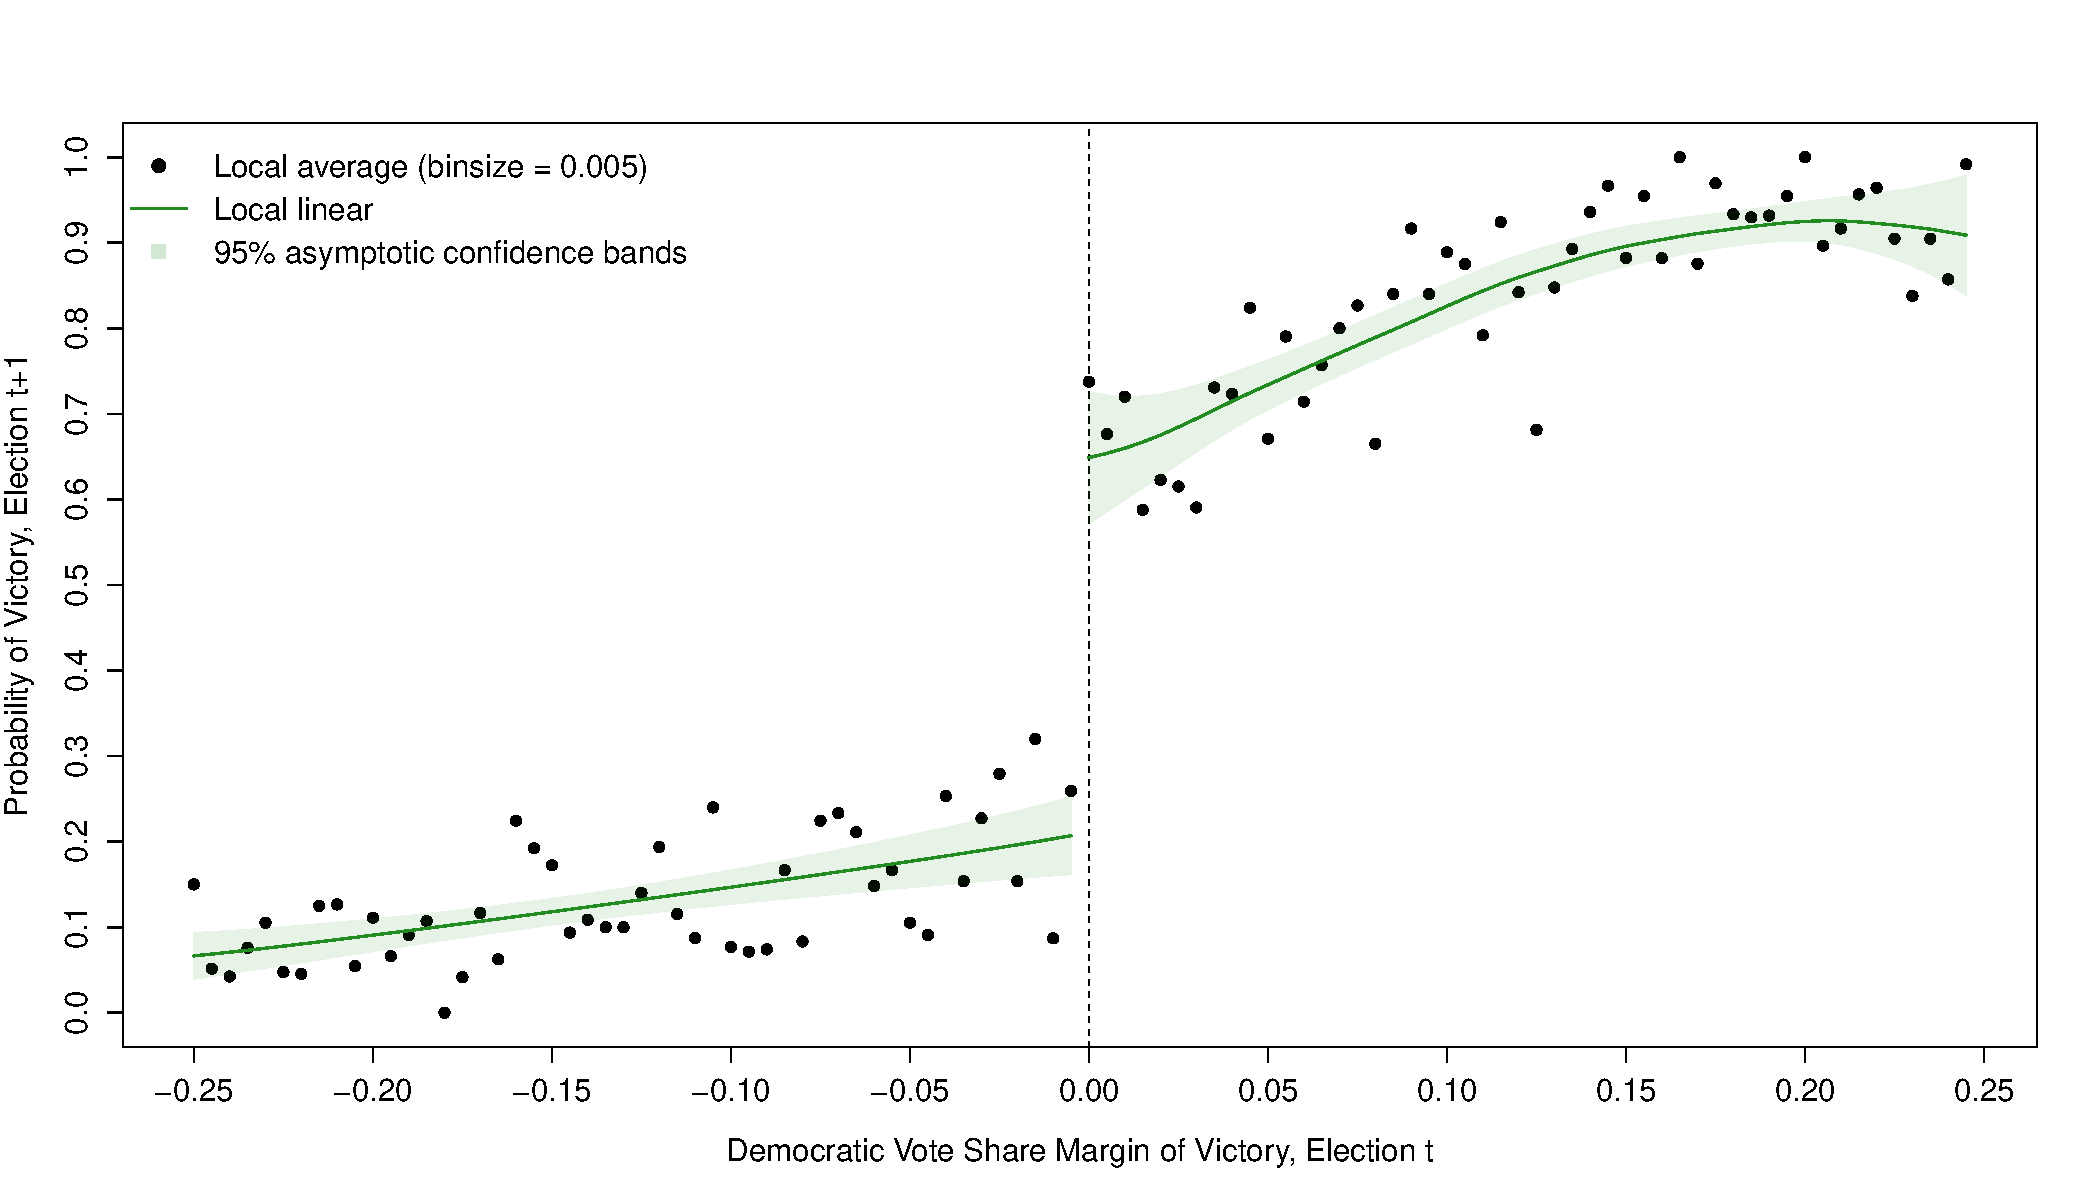
\includegraphics[trim=0 15 20 50, clip, width=0.75\textwidth]{figure_06.pdf}
	\caption{Democrats' probability of victory in election $t+1$, by margin of victory in election $t$.
			 LL estimate along with 95\% approximate confidence bands.}
	\label{fig:application_confidence_bands}
\end{figure}
% TeX file "conclusion"

% Research Module in Econometrics & Statistics 
% Prof. Dr. Liebl & Dr. Christopher Walsh
% Winter 2021/22, M.Sc. Economics, Bonn University
% Xingyu Tao, Xuan Li, Sven Jacobs


\section{Conclusion} \label{sec:conclusion}

The paper discussed boundary effects in kernel regression.
We have seen that the Nadaraya-Watson estimator in general suffers from poor boundary behavior.
This is visually disturbing,
but also manifests in a larger order of the bias and thus a slower rate of convergence compared to the interior.
We focused on two methods to overcome the boundary problem.
Local linear regression preserves the order of the interior and was shown, theoretically and graphically,
to correct the bias exactly to first order.
The second approach, applying special boundary kernels when estimating in boundary regions,
instead provides an asymptotic bias adjustment.

A Monte-Carlo simulation study showed that the local linear estimator performs better than the boundary-adjusted Nadaraya-Watson estimator,
particularly for small sample sizes and non-uniform designs.
Moreover, the study revealed the relative advantage of Nadaraya-Watson for boundary estimation when estimation variability is the dominant component,
i.e.\ when the effective sample size is small or the regression function is rather flat.
A real-data application of the methods to determine the size of a causal effect in the RDD illustrated the need for boundary correction in practice,
as boundary effects can substantially bias estimates and inference.

Overall, in econometrics boundaries are often of special interest and the potential severe bias of Nadaraya-Watson then requires an adjustment.
Boundary kernels achieve an asymptotic correction,
but are rather complicated and tedious to implement in practice.
Local linear regression, in contrast, is a simple and intuitive method which automatically adapts to estimation at boundaries.
Besides, it has the favorable design-adaptivity property.
Therefore, we recommend local linear regression.

We restricted our analysis to the Nadaraya-Watson and the local linear estimator as two special cases of the local polynomial estimator to obtain the key insights.
Higher-order polynomials can further reduce the bias,
but at the expense of increased variability.
In practical applications often the local linear estimator is chosen.
An interesting extension of our research is to investigate boundary effects in higher dimensions.
Especially because the boundary region is larger and boundary effects may occur over much of the domain.
In fact, the fraction of points close to the boundary increases to one as the dimension grows \parencite[200]{Hastie_2009}.
Another possible extension is the estimation of curves that depend on the regression function,
e.g.\ derivatives.

\clearpage

% TeX file "appendix"

% Research Module in Econometrics & Statistics 
% Prof. Dr. Liebl & Dr. Christopher Walsh
% Winter 2021/22, M.Sc. Economics, Bonn University
% Xingyu Tao, Xuan Li, Sven Jacobs


\phantomsection 
\addcontentsline{toc}{section}{Appendix} 

\section*{Appendix}

\subsection*{Appendix 1: Proofs} \label{appendix_1}

\begin{proof}[Proof (Theorem \ref{theorem_1})]
	Fix some $x$ in the interior of $\supp(f)$.
	We write
	\begin{align}
		Y_i &= m(X_i) + \epsilon_i \\
		    &= m(x) + [m(X_i) - m(x)] + \epsilon_i \,.
	\end{align}
	It then also holds that
	\begin{align}
		\frac{1}{nh} \sum_{i = 1}^{n} K \left( \frac{X_i - x}{h} \right) Y_i &=
		\frac{1}{nh} \sum_{i = 1}^{n} K \left( \frac{X_i - x}{h} \right) m(x) \\
		&+ \underbrace{\frac{1}{nh} \sum_{i = 1}^{n} K \left( \frac{X_i - x}{h} \right) [m(X_i) - m(x)]}_{\equiv \, \hat{g}_1(x)} +
		\underbrace{\frac{1}{nh} \sum_{i = 1}^{n} K \left( \frac{X_i - x}{h} \right) \epsilon_i}_{\equiv \, \hat{g}_2(x)} \,.  
	\end{align}
	Dividing by the standard kernel density estimator $\hat{f}(x)$ yields
	\begin{equation}
		\hat{m}_{\NW}(x) = m(x) + \frac{\hat{g}_1(x)}{\hat{f}(x)} + \frac{\hat{g}_2(x)}{\hat{f}(x)} \,. \label{eq:appendix_1_01}
	\end{equation}
	
	We first derive $\E[\hat{m}_{\NW}(x) \,|\, \bm{X}]$.
	Since $\E[\epsilon_i \,|\, X_i] = 0$, we immediately get $\E[\hat{g}_2(x) \,|\, \bm{X}] = 0$.
	For $\hat{g}_1(x)$ we have
	\begin{equation}
		\E[\hat{g}_1(x) \,|\, \bm{X}] = \frac{1}{h} \E \left[ K \left( \frac{X - x}{h}  \right) [m(X) - m(x)] \right] \,.
	\end{equation}
	Writing the expectation as an integral with respect to the design density $f$ and applying variable substitution leads to
	\begin{align}
		\E[\hat{g}_1(x) \,|\, \bm{X}] &= \int_{-\infty}^{\infty} \frac{1}{h} K \left( \frac{z - x}{h} \right) [m(z) - m(x)] f(z) \diff z \\
		&= \int_{-\infty}^{\infty} K(u) [m(x + hu) - m(x)] f(x + hu) \diff u \,. \label{eq:appendix_1_02}
	\end{align}
	In the next step we write $m(x + hu)$ and $f(x + hu)$ as Taylor expansions around $x$:
	\begin{align}
		m(x + hu) &= m(x) + m'(x)hu + \frac{1}{2} m''(x)h^2u^2 + \littleO(h^2) \,, \\
		f(x + hu) &= f(x) + f'(x)hu + \littleO(h) \,.
	\end{align} 
	Plugged into \eqref{eq:appendix_1_02} we obtain
	\begin{align}
		\E[\hat{g}_1(x) \,|\, \bm{X}] &= \int_{-\infty}^{\infty} K(u) \left[ m'(x)hu + \frac{1}{2} m''(x)h^2u^2 + \littleO(h^2) \right] [f(x) + f'(x)hu + \littleO(h)] \diff u \label{eq:appendix_1_03} \\ 
		&= h \int_{-\infty}^{\infty} uK(u) \diff u \, m'(x) [f(x) + \littleO(h)] \label{eq:appendix_1_04} \\
		&+ h^2 \int_{-\infty}^{\infty} u^2K(u) \diff u \left[ \frac{1}{2} m''(x) f(x) + m'(x) f'(x) \right] \\
		&+ h^3 \int_{-\infty}^{\infty} u^3K(u) \diff u \, \frac{1}{2} m''(x) f'(x) \\
		&+ \littleO(h^2) \,.
	\end{align}
	Due to the symmetry of the kernel from Assumption \ref{A4} odd kernel moments vanish. Hence, we can write with the definition of $\kappa_2(K)$ 
	\begin{equation}
		\E[\hat{g}_1(x) \,|\, \bm{X}] = \frac{1}{2} \kappa_2(K) m''(x) h^2 f(x) + \kappa_2(K) m'(x)f'(x) h^2 + \littleO(h^2) \,.
	\end{equation}
	With \eqref{eq:appendix_1_01} and the consistency of the kernel density estimator \parencite{Parzen_1962}, i.e.\ $\hat{f}(x) \overset{p}{\longrightarrow} f(x)$,
	we arrive at the desired expression
	\begin{equation}
		\ABias (\hat{m}_{\NW}(x) \,|\, \bm{X}) = \frac{1}{2} \kappa_2(K) m''(x) h^2 + \kappa_2(K) \frac{m'(x)f'(x)}{f(x)} h^2 \,.	
	\end{equation}

	We now derive $\Var(\hat{m}_{\NW}(x) \,|\, \bm{X})$.
	For $\hat{g}_2(x)$ we get
	\begin{align}
		\Var(\hat{g}_2(x)) &= \frac{1}{nh^2} \E \left[ K \left( \frac{X_i - x}{h} \right) \epsilon_i \right]^2 \,, \\
		\Var(\hat{g}_2(x) \,|\, \bm{X}) &= \frac{1}{nh^2} \E \left[ K \left( \frac{X_i - x}{h} \right)^2 \sigma^2(X_i) \right] \,.
	\end{align}
	Writing the expectation as an integral with respect to the design density $f$ and applying variable substitution leads to
	\begin{align}
		\Var(\hat{g}_2(x) \,|\, \bm{X}) &= \frac{1}{nh^2} \int_{-\infty}^{\infty} K \left( \frac{z - x}{h} \right)^2 \sigma^2(z) f(z) \diff z \\
		&= \frac{1}{nh} \int_{-\infty}^{\infty} K(u)^2 \sigma^2(x + hu) f(x + hu) \diff u \,.
	\end{align}
	Writing $\sigma^2(x + hu)$ and $f(x + hu)$ as first-order Taylor expansions around $x$ and using the definition of $R(K)$ we arrive at
	\begin{equation}
		\Var(\hat{g}_2(x) \,|\, \bm{X}) = R(K) \sigma^2(x) f(x) \frac{1}{nh} + \littleO \left( \frac{1}{nh} \right) \,.
	\end{equation}
	For $\hat{g}_1(x)$ a similar expansion as was done for its expectation yields $\Var(\hat{g}_1(x) \,|\, \bm{X}) \sim \frac{h^2}{nh}$ which is of smaller order than $(nh)^{-1}$.
	With \eqref{eq:appendix_1_01} and $\hat{f}(x) \overset{p}{\longrightarrow} f(x)$ we obtain the desired expression
	\begin{equation}
		\AVar (\hat{m}_{\NW}(x) \,|\, \bm{X}) = \frac{R(K) \sigma^2(x)}{f(x)} \frac{1}{nh} \,.
	\end{equation} 
\end{proof}

\begin{proof}[Proof (Theorem \ref{theorem_4})]
	In Section \ref{subsec:definition} we have seen that
	\begin{equation}
		\hat{m}_{\LL}(x) = \bm{e}_1^\top \left( \bm{X}_x^\top \bm{W}_x^{\vphantom{\top}} \bm{X}_x^{\vphantom{\top}} \right)^{-1} \bm{X}_x^\top \bm{W}_x^{\vphantom{\top}} \bm{Y} \,.
	\end{equation}
	The general solution of the local polynomial estimator of degree $p$ can be computed as (e.g.\ \cite{Hastie_1993})
	\begin{align}
		\hat{m}_{\LP}(x; p) &= \bm{b}_x^\top \left( \bm{\tilde{X}}_x^\top \bm{W}_x^{\vphantom{\top}} \bm{\tilde{X}}_x^{\vphantom{\top}} \right)^{-1} \bm{\tilde{X}}_x^\top \bm{W}_x^{\vphantom{\top}} \bm{Y} \\
							&= \sum_{i = 1}^{n} w_i(x) Y_i \,,
	\end{align}
	where invertibility of $\bm{\tilde{X}}_x^\top \bm{W}_x^{\vphantom{\top}} \bm{\tilde{X}}_x^{\vphantom{\top}}$ is assumed and
	\begin{equation}
		\bm{Y} = \begin{bmatrix} Y_1 \\ \vdots \\ Y_n \end{bmatrix},
		\bm{\tilde{X}}_x = \begin{bmatrix} 1 & X_1 & \dots & X_1^p \\ \vdots & \vdots & \ddots & \vdots \\ 1 & X_n & \dots & X_n^p \end{bmatrix},
		\bm{W}_x = \diag \left\{ K \left( \frac{X_1 - x}{h} \right), \dots, K \left( \frac{X_n - x}{h} \right) \right\},
		\bm{b}_x = \begin{bmatrix} 1 \\ x \\ \vdots \\ x^p \end{bmatrix} \,.
	\end{equation}
	With $\bm{v}_j^\top \equiv (X_1^j, X_2^j, \dots, X_n^j)$ for $j = 0, 1, \dots, p$ we can write
	\begin{equation} \label{eq:appendix_1_05}
		\bm{b}_x^\top \left( \bm{\tilde{X}}_x^\top \bm{W}_x^{\vphantom{\top}} \bm{\tilde{X}}_x^{\vphantom{\top}} \right)^{-1} \bm{\tilde{X}}_x^\top \bm{W}_x^{\vphantom{\top}} \bm{v}_j = \sum_{i = 1}^{n} w_i(x) X_i^j \,.
	\end{equation}
	Applying \eqref{eq:appendix_1_05} for each $j = 0, 1, \dots, p$ and noticing that $\bm{\tilde{X}}_x = [\bm{v}_0, \bm{v}_1, \dots, \bm{v}_p]$ gives for the LHS of \eqref{eq:appendix_1_05}
	\begin{align}
		&\bm{b}_x^\top \left( \bm{\tilde{X}}_x^\top \bm{W}_x^{\vphantom{\top}} \bm{\tilde{X}}_x^{\vphantom{\top}} \right)^{-1} \bm{\tilde{X}}_x^\top \bm{W}_x^{\vphantom{\top}} \bm{\tilde{X}}_x^{\vphantom{\top}} \\
		= \,\, &\bm{b}_x^\top \\
		= \,\, &[1, x, \dots, x^p]
	\end{align}
	and for the RHS
	\begin{equation}
		\left[ \sum_{i = 1}^{n} w_i(x), \sum_{i = 1}^{n} w_i(x) X_i, \dots, \sum_{i = 1}^{n} w_i(x) X_i^p \right] \,.
	\end{equation}
	By component matching we obtain
	\begin{equation}
		x^j = \sum_{i = 1}^{n} w_i(x) X_i^j \,,
	\end{equation}
	such that for $j = 0$ and $j = 1$:
	\begin{align}
		1 &= \sum_{i = 1}^{n} w_i(x) \,, \\
		x &= \sum_{i = 1}^{n} w_i(x) X_i \,.
	\end{align}
	If we combine these two equations (multiplying the first by $x$) we arrive at the desired result
	\begin{equation}
		\sum_{i = 1}^{n} w_i(x) (X_i - x) = 0 \,.
	\end{equation} 
\end{proof}

\newpage

\subsection*{Appendix 2: Kernels} \label{appendix_2}

The following is a short excursus on the optimal kernel choice.
When calculating the minimal asymptotic error functions $\AMSE_{\text{opt}}$ and $\AMISE_{\text{opt}}$ following Section~\ref{subsec:theoretical_comparison}, the dependence on the kernel can be seen to be $R(K)^{4/5} \kappa_2(K)^{2/5}$.
This dependence is the same for kernel density estimation \parencite[49]{Müller_1988}.
The kernel minimizing the expression is the Epanechnikov kernel $K_\text{E}(u) = \frac{3}{4}(1 - u^2)$ as was proved first by \textcite{Epanechnikov_1969} in the context of density estimation.
The efficiency of a kernel is then defined relative to the optimal Epanechnikov kernel by 
\begin{equation}
	\Eff(K) \equiv \frac{R(K_{\text{E}}) \kappa_2(K_{\text{E}})^{1/2}}{R(K) \kappa_2(K)^{1/2}} \,.
\end{equation}
Table~\ref{tab:kernels} lists the efficiency scores for kernels mostly applied in practice.
\textcite[Section~5]{Müller_1988} provides a thorough treatment of optimal kernel theory including, for instance, optimal higher-order kernel functions.
\vfill
\renewcommand{\arraystretch}{1.4}	
\begin{table}[h]
	\centering
	\captionabove{Prominent kernels with their constants and efficiency}
	\label{tab:kernels}
	\begin{tabular}{l l c c c c}  
		\toprule
		Kernel & Function & Support & $R(K)$ & $\kappa_2(K)$ & Efficiency \\
		\midrule
		Epanechnikov & $K_\text{E}(u) = \frac{3}{4}(1 - u^2)$                     & $[-1, 1]$    & $\frac{3}{5}$           & $\frac{1}{5}$ & 100.0\% \\
		Biweight     & $K_\text{B}(u) = \frac{15}{16}{(1 - u^2)}^2$               & $[-1, 1]$    & $\frac{5}{7}$           & $\frac{1}{7}$ & 99.39\% \\
		Triangular   & $K_\text{T}(u) = 1 - |u|$                                  & $[-1, 1]$    & $\frac{2}{3}$           & $\frac{1}{6}$ & 98.59\% \\
		Gaussian     & $K_\text{G}(u) = \frac{1}{\sqrt{2\pi}}\e^{-\frac{u^2}{2}}$ & $\mathbb{R}$ & $\frac{1}{2\sqrt{\pi}}$ & $1$           & 95.12\% \\
		Uniform      & $K_\text{U}(u) = \frac{1}{2}$                              & $[-1, 1]$    & $\frac{1}{2}$           & $\frac{1}{3}$ & 92.95\% \\
		\bottomrule
	\end{tabular}	
\end{table}
\renewcommand{\arraystretch}{1.0}
\vfill
\begin{figure}[h]
	\centering	
	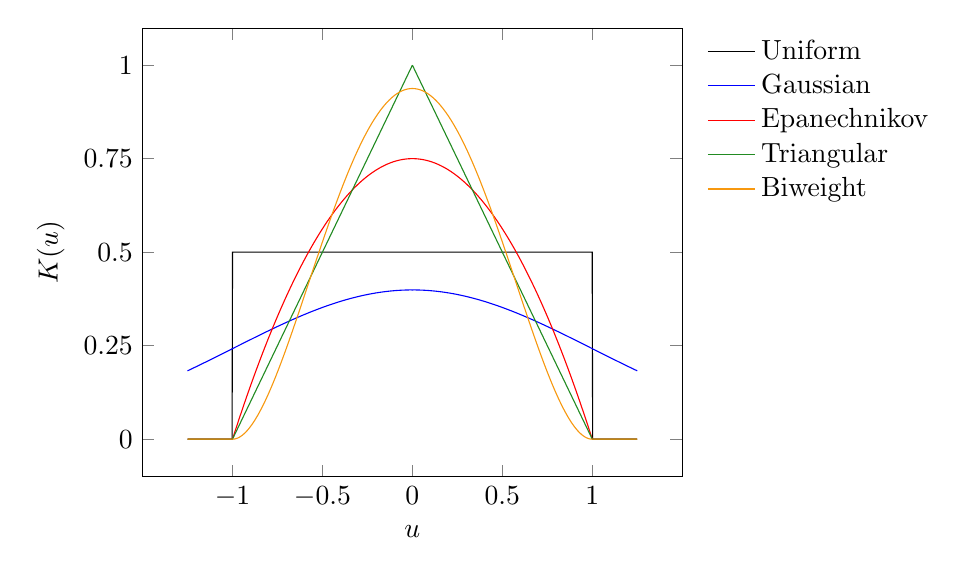
\begin{tikzpicture}
		\begin{axis}
			[
			grid, grid style={white}, 
			samples=1000, 
			domain=-1.25:1.25, 
			xlabel=$u$, xtick={-1, -0.5, 0, 0.5, 1},
			ylabel=$K(u)$, ytick={0, 0.25, 0.5, 0.75, 1},
			legend entries={Uniform, Gaussian, Epanechnikov, Triangular, Biweight},
			legend pos=outer north east,
			legend style={draw=none}, legend cell align={left}
			]
			
			\addplot[black]
			expression {1/2 * (abs(x)<1)};
			
			\addplot[blue]
			expression {1/(sqrt(2*pi)) * exp(-1/2*x^2)};
			
			\addplot[red]
			expression {3/4 * (1 - x^2) * (abs(x)<1)};
			
			\addplot[ForestGreen]
			expression {(1 - abs(x)) * (abs(x)<1)};
			
			\addplot[YellowOrange]
			expression {15/16 * (1 - x^2)^2 * (abs(x)<1)};
		\end{axis}
	\end{tikzpicture}
	\caption{Prominent kernels as given in Table~\ref{tab:kernels}}
\end{figure}

\newpage

\subsection*{Appendix 3: Additional material -- Theoretical description}
\vfill
\begin{figure}[h]
	\centering
	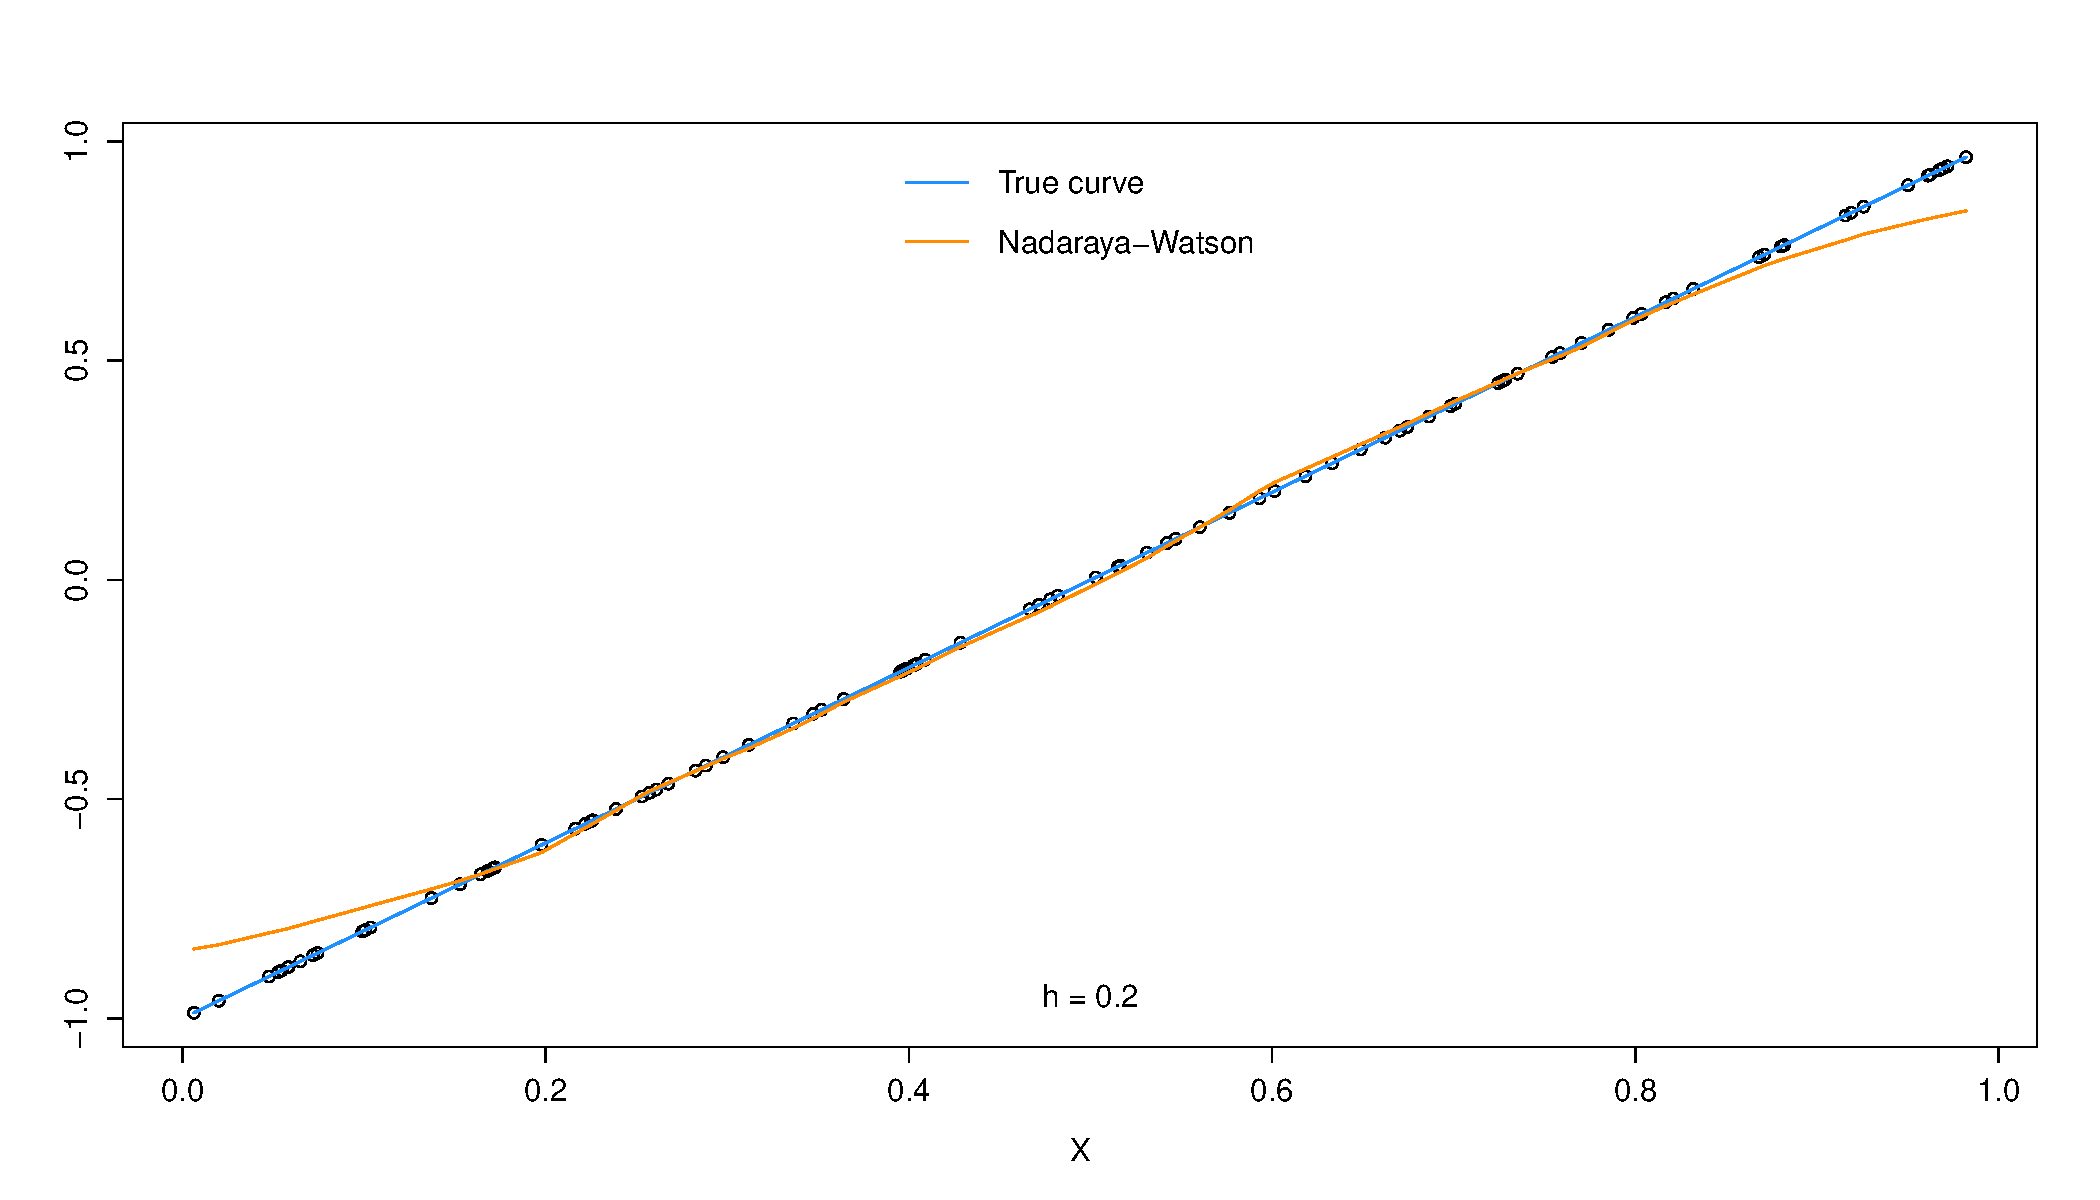
\includegraphics[trim=20 15 20 50, clip, width=0.75\textwidth]{figure_08.pdf}
	\caption{Nadaraya-Watson estimator in the case of linear regression, $m(x) = -1 + 2x$.
			 The realizations of $X$ are drawn from a uniform distribution and for clarification no noise is added.
		 	 The boundary effects are clearly visible, namely the bending of the straight line to a constant at the edges.}
	\label{fig:boundary_effects_linear}
\end{figure}
\vfill
\begin{figure}[h]
	\centering
	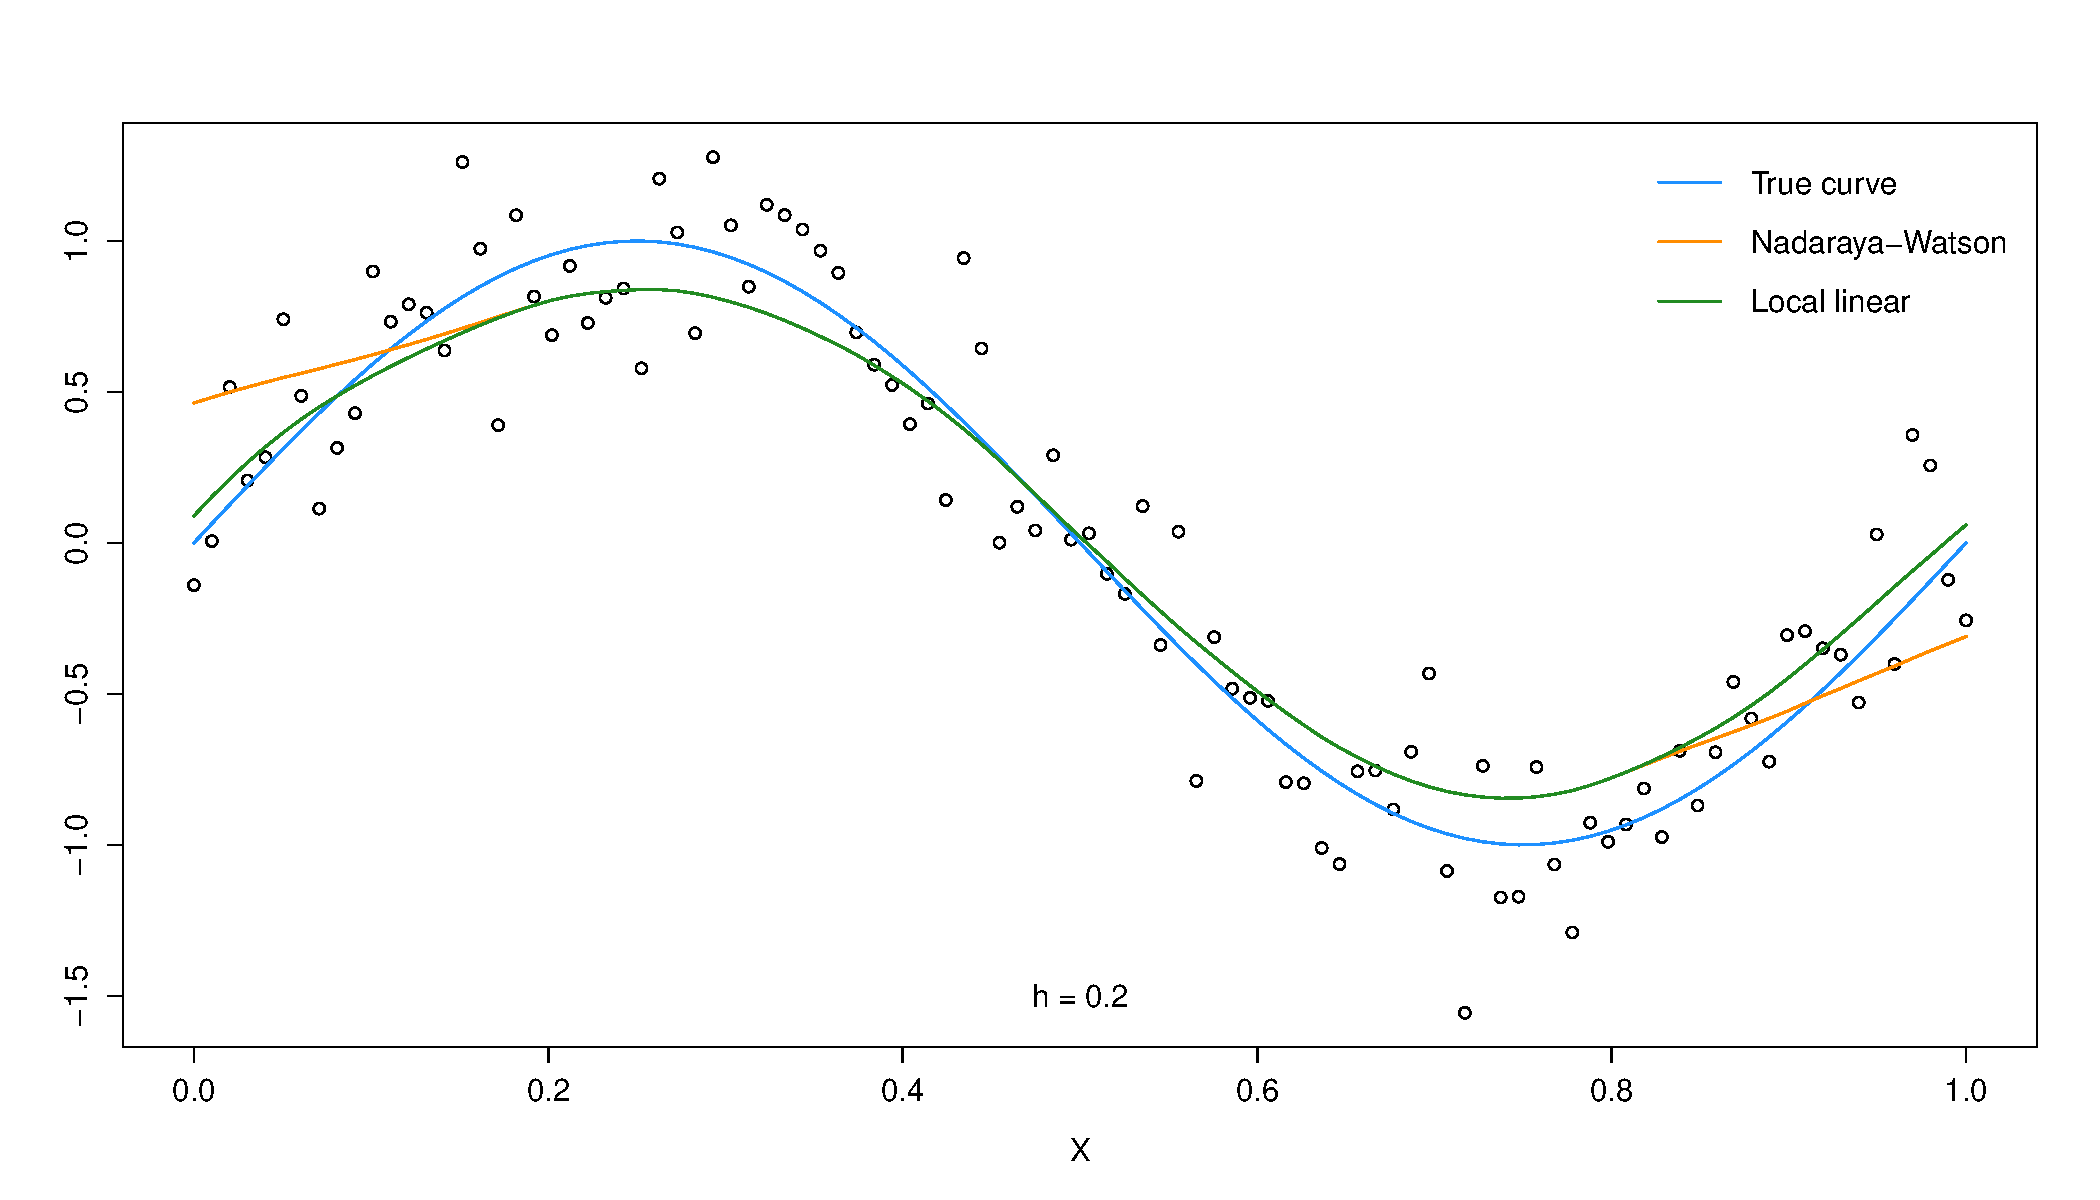
\includegraphics[trim=20 15 20 50, clip, width=0.75\textwidth]{figure_09.pdf}
	\caption{Local linear estimator compared to the Nadaraya-Watson estimator for 100 simulated observations}
	\label{fig:ll}
\end{figure}
\vfill
\begin{figure}
	\centering
	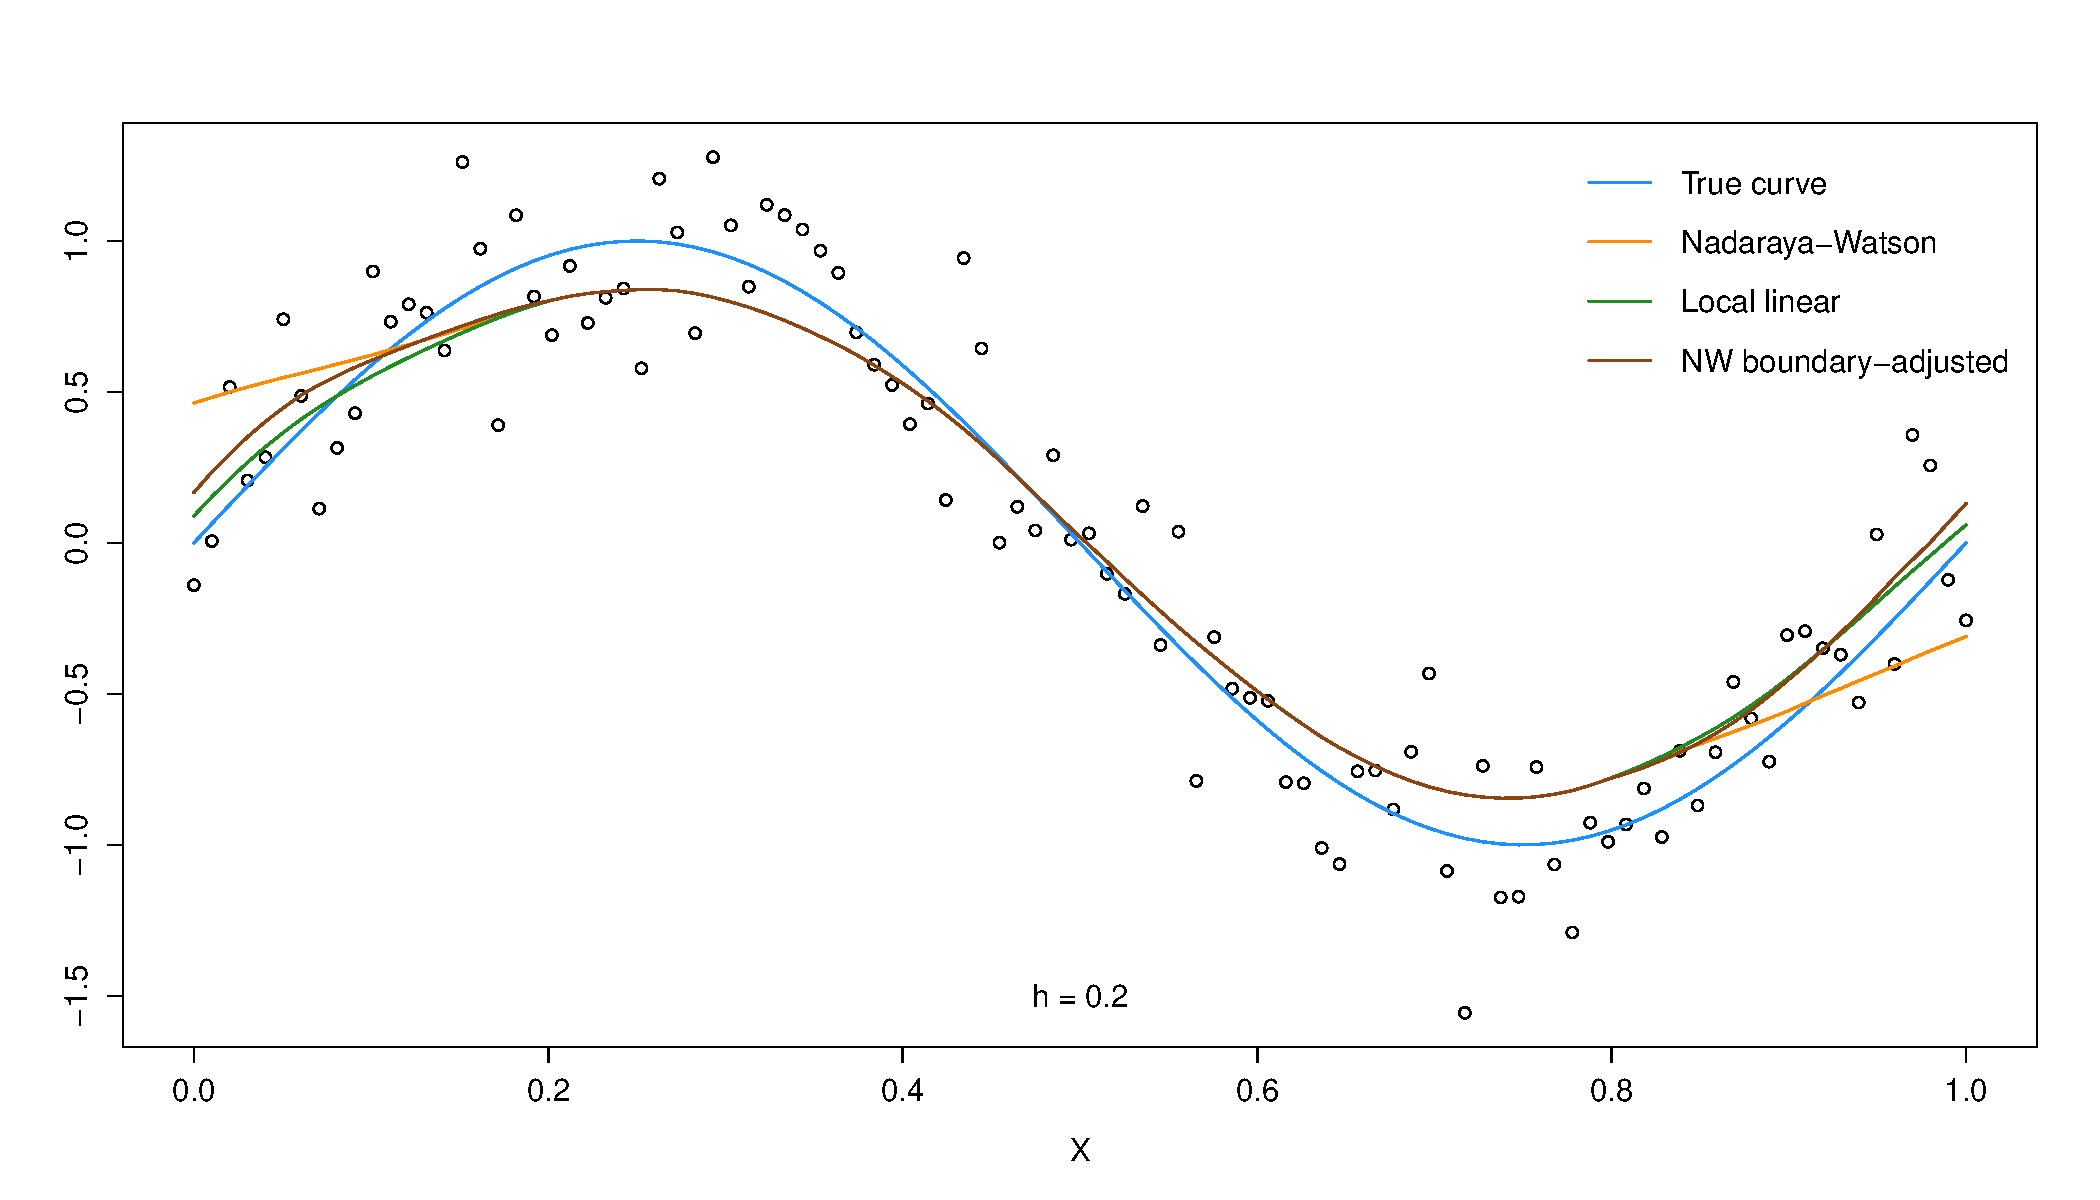
\includegraphics[trim=20 15 20 50, clip, width=0.75\textwidth]{figure_10.pdf}
	\caption{Boundary-adjusted Nadaraya-Watson estimator compared to the standard Nadaraya-Watson estimator and the local linear estimator for 100 simulated observations.
			 For explicit boundary adjustment the Epanechnikov boundary kernel from Section~\ref{sec:boundary_kernels} is used.}
	\label{fig:nw_boundary_adjusted}
\end{figure}

\begin{figure}
	\centering
	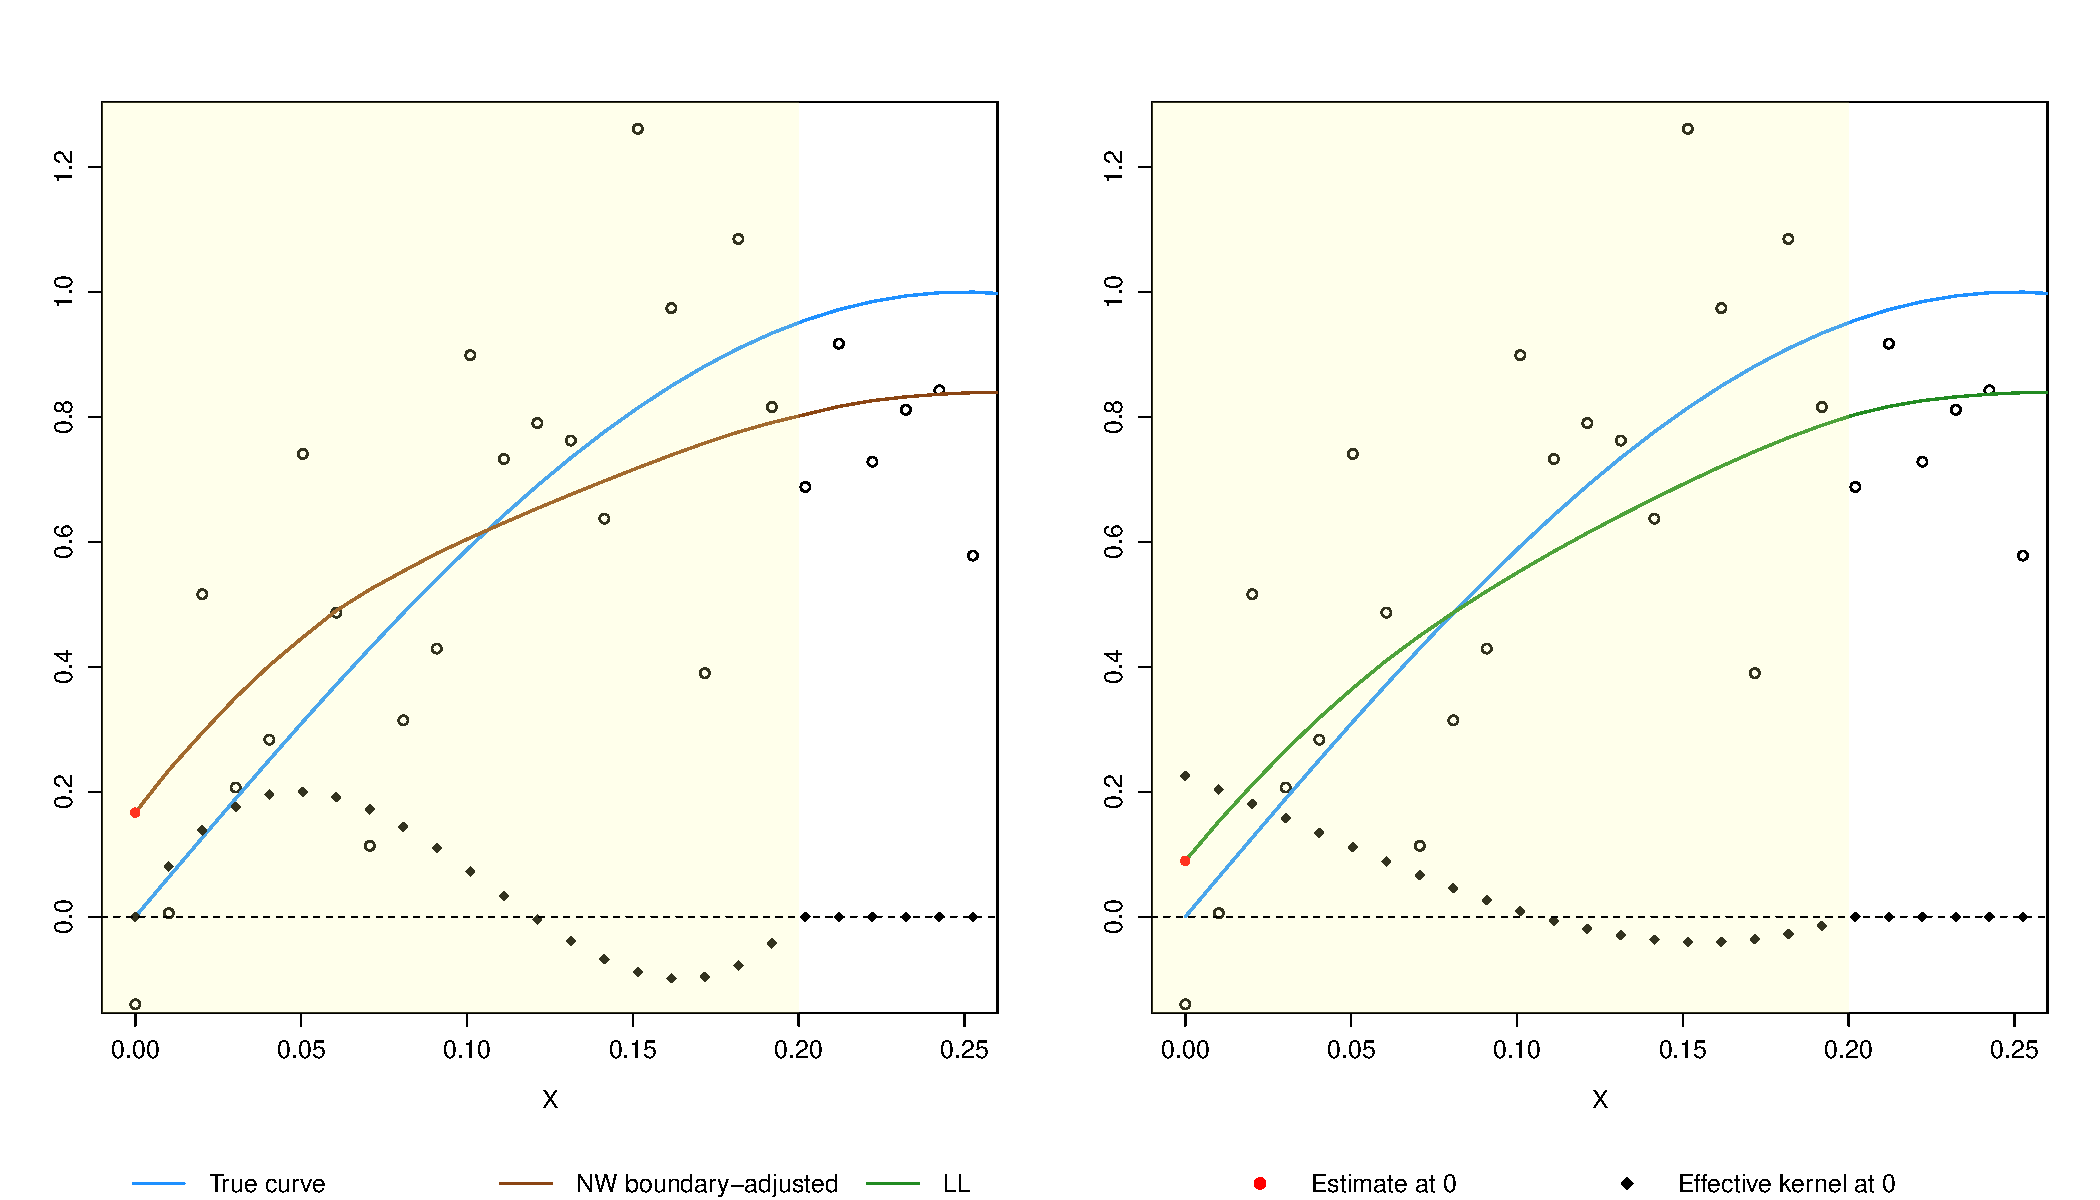
\includegraphics[trim=20 0 20 45, clip, width=0.75\textwidth]{figure_11.pdf}
	\caption{Effective kernel for the boundary-adjusted Nadaraya-Watson estimator and the local linear estimator when estimating at the lower boundary $x = 0$.
			 The effective kernel is given by the filled squares.}
	\label{fig:effective_kernel_nw_boundary}
\end{figure}

\clearpage

\subsection*{Appendix 4: Additional material -- Simulation}
\vfill
\begin{figure}[h!]
	\centering
	\begin{subfigure}{\textwidth}
		\centering
		\begin{tikzpicture}
			\begin{axis}
				[
				grid, grid style={white}, 
				samples=1000, 
				domain=0:1
				]
			
				\addplot[black]
				expression {sin(deg(2*pi*x))};
			\end{axis}
		\end{tikzpicture}
		\caption{$m_1(x) = \sin(2 \pi x)$ on the interval $[0, 1]$}
		\label{fig:m_1}
	\end{subfigure}
	\\[2ex]
	\begin{subfigure}{\textwidth}
		\centering
		\begin{tikzpicture}
			\begin{axis}
				[
				grid, grid style={white}, 
				samples=1000, 
				domain=0:1
				]
		
				\addplot[black]
				expression {2 - 2*x + 2*exp(-(x - 0.5)^2 / 0.01)};
			\end{axis}
		\end{tikzpicture}
		\caption{$m_2(x) = 2 - 2x + 2\exp \{ - (x - 0.5)^2 / 0.01 \} $ on the interval $[0, 1]$}
		\label{fig:m_2}
	\end{subfigure}
	\\[2ex]
	\begin{subfigure}{\textwidth}
		\centering
		\begin{tikzpicture}
			\begin{axis}
				[
				grid, grid style={white}, 
				samples=1000, 
				domain=0:1
				]
		
				\addplot[black]
				expression {2 - 2*x + 2*exp(-(x - 0)^2 / 0.01)};
			\end{axis}
		\end{tikzpicture}
		\caption{$m_3(x) = 2 - 2x + 2\exp \{ - (x - 0)^2 / 0.01 \} $ on the interval $[0, 1]$}
		\label{fig:m_3}
	\end{subfigure}
	\caption{Regression functions chosen for the simulation study}
	\label{fig:simulation_functions}
\end{figure}
\vfill
\begin{figure}
	\centering
	\begin{tikzpicture}
		\begin{axis}
			[
			grid, grid style={white}, 
			samples=1000, 
			domain=-0.25:1.25
			]
			
			\addplot[black]
			expression {3*(5/12 - (x - 0.5)^2) * (x>0) * (x<1)};
		\end{axis}
	\end{tikzpicture}
	\caption{Clustered design density $f_{\ast}$}
	\label{fig:clustered_design_density}
\end{figure}

\begin{figure}
	\centering
	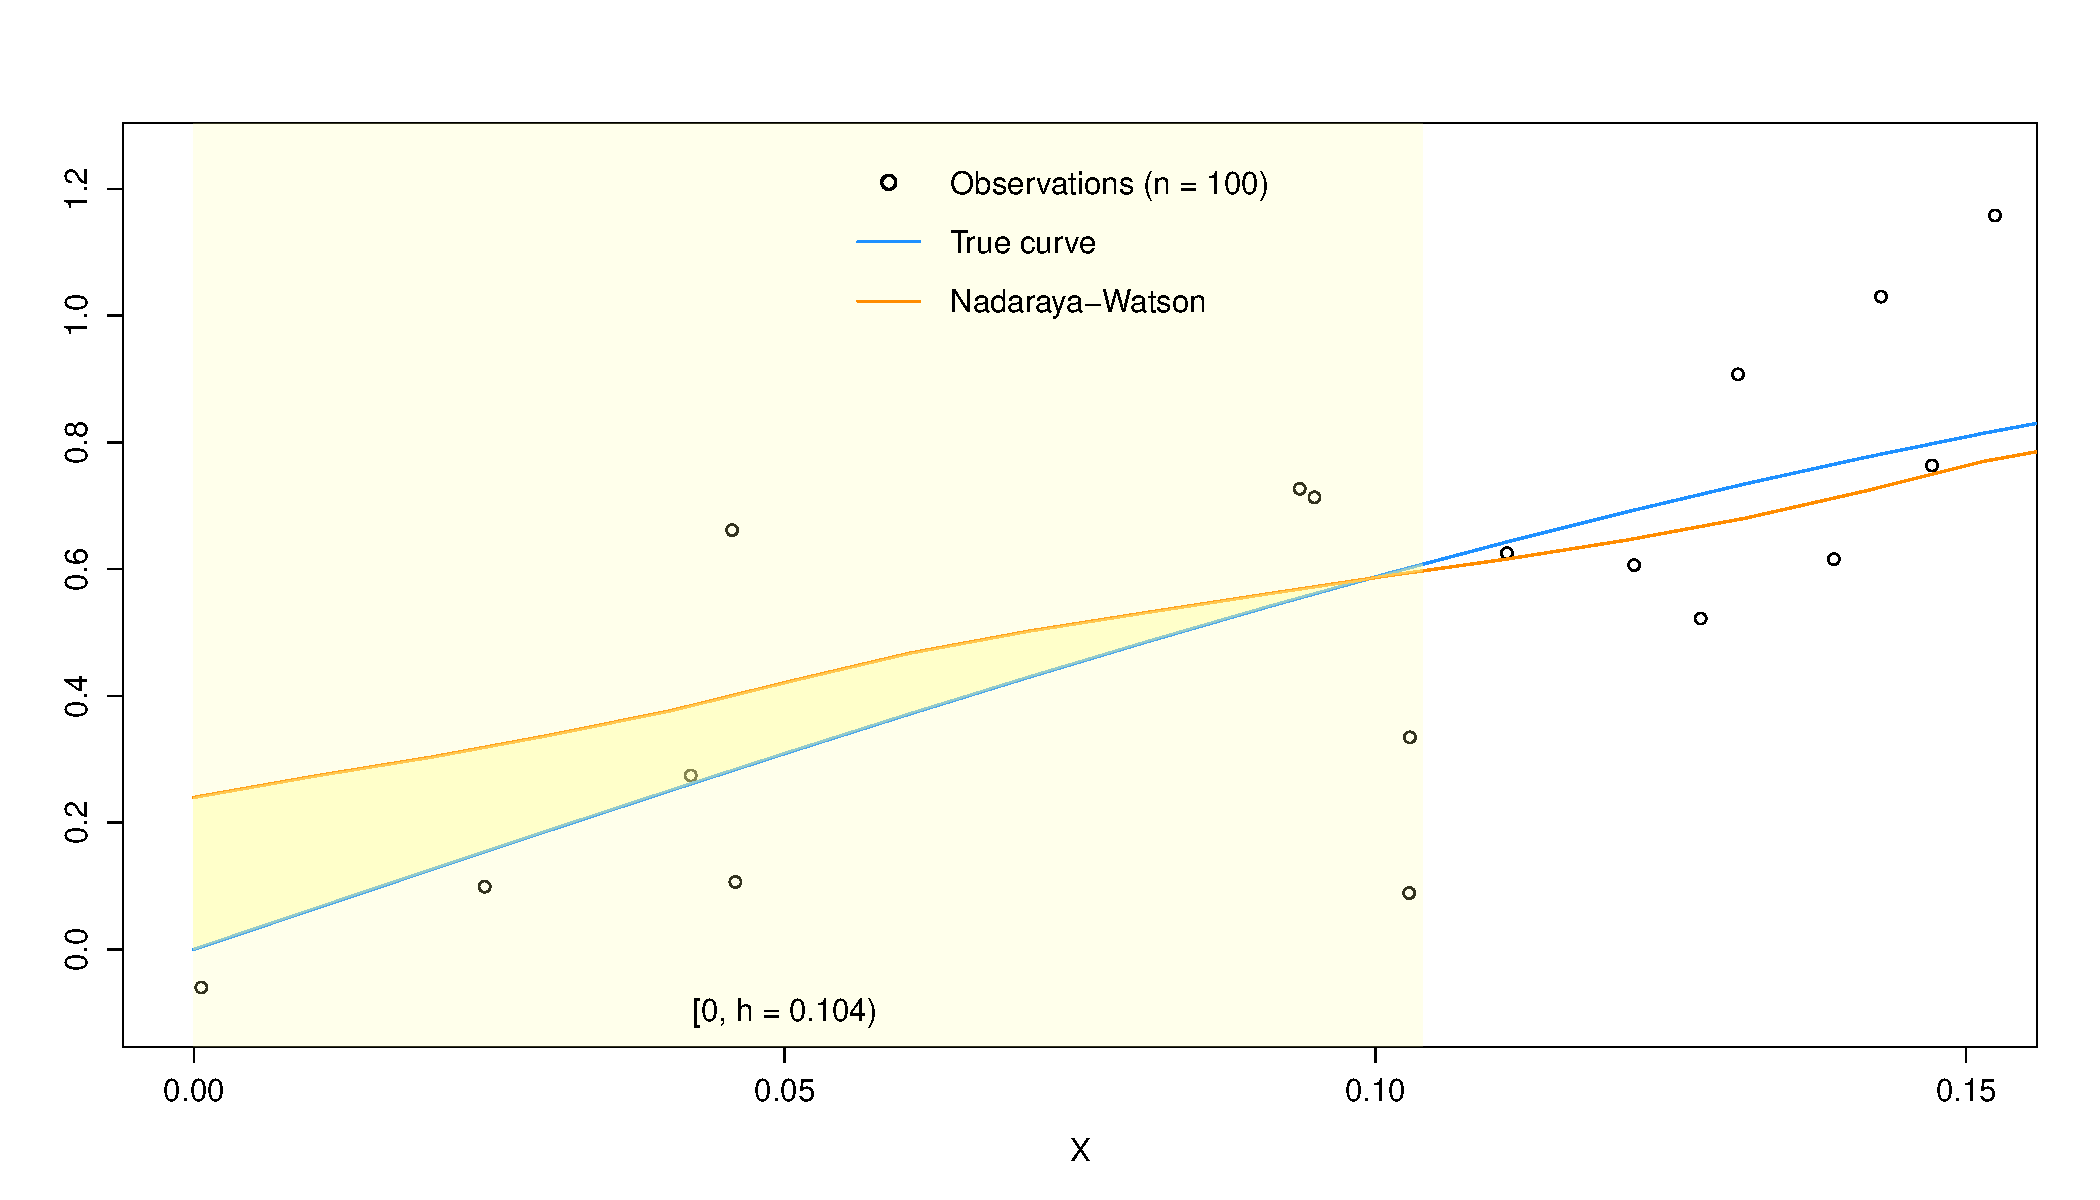
\includegraphics[trim=20 15 20 50, clip, width=0.75\textwidth]{figure_14.pdf}
	\caption{Nadaraya-Watson fit and the regression function $m_1$ over the left boundary region (yellow-shaded),
			 for a random sample of $n = 100$ observations.
			 The dark yellow area reflects the integrated error.}
	\label{fig:simulation_set-up}
\end{figure}

\clearpage

\subsection*{Appendix 5: Additional material -- Application}
\vfill
\begin{figure}[h]
	\centering
	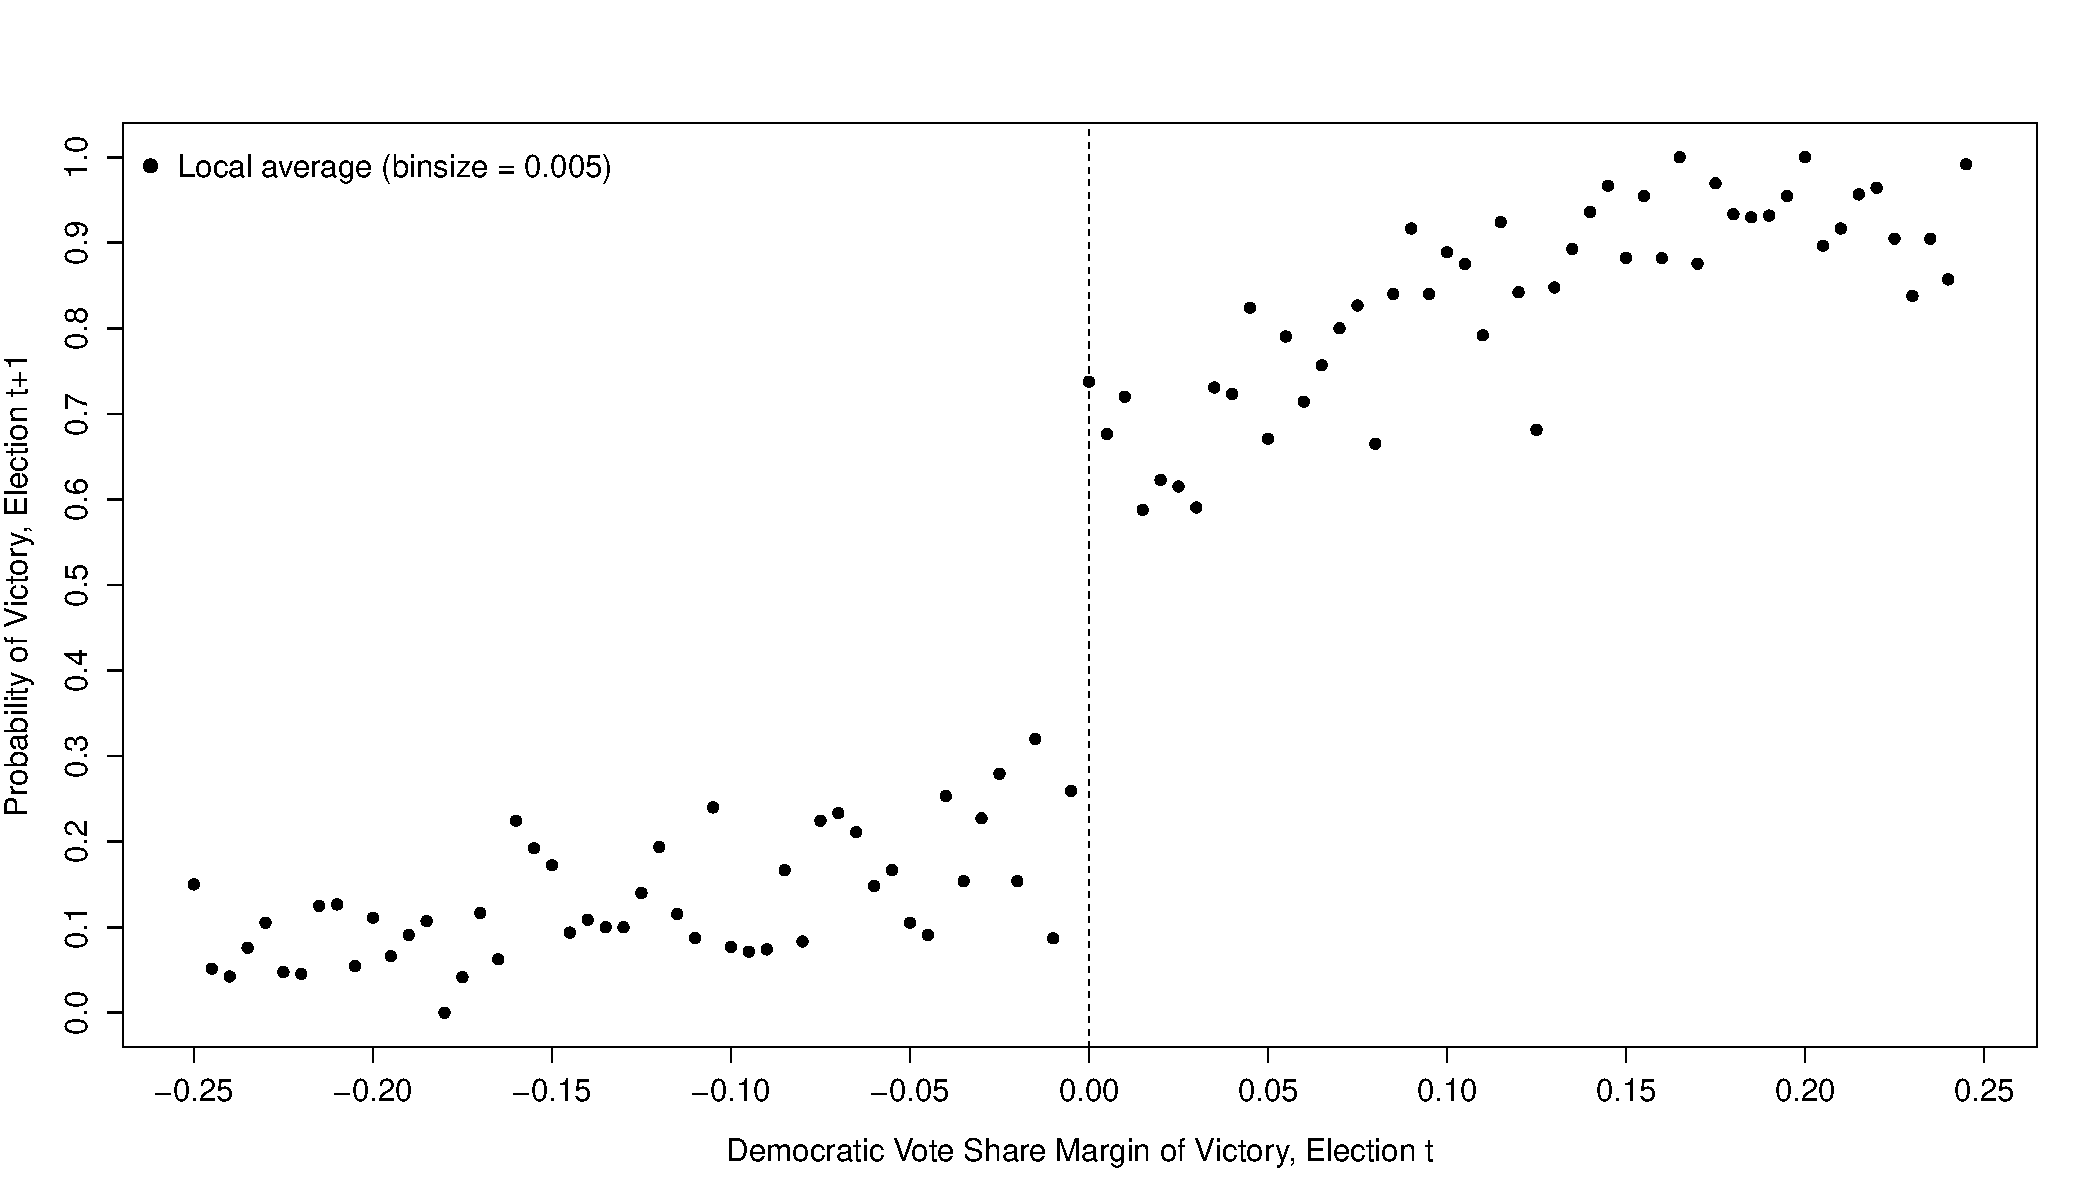
\includegraphics[trim=0 15 20 50, clip, width=0.75\textwidth]{figure_15.pdf}
	\caption{Democrats' probability of victory in election $t+1$, by margin of victory in election $t$.
			 Local averages are given by the filled circles.}
	\label{fig:application_overview}
\end{figure}
\vfill
\begin{figure}
	\centering
	\begin{subfigure}{0.75\textwidth}
		\centering
		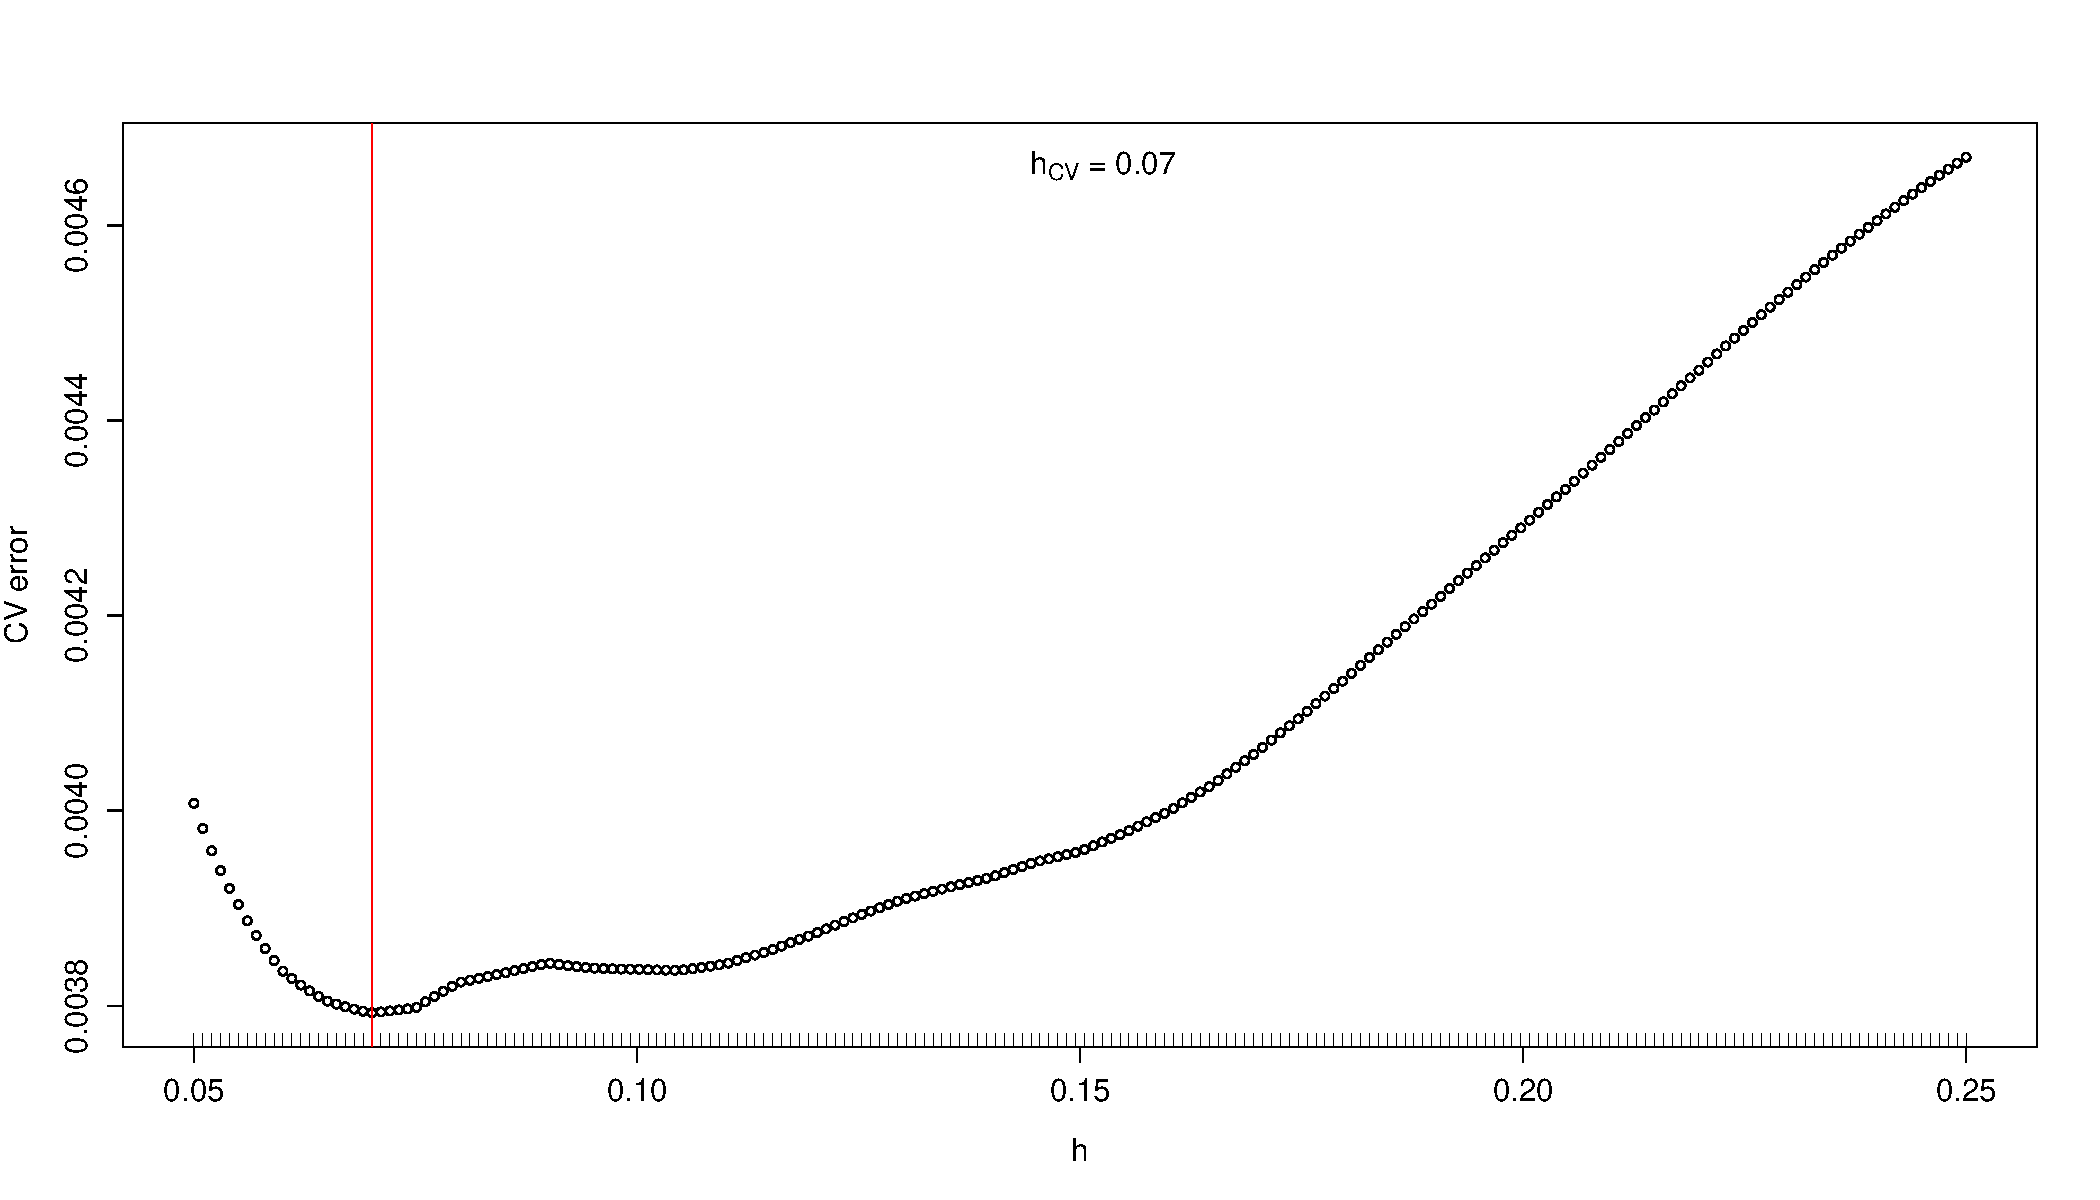
\includegraphics[trim=0 0 20 45, clip, width=\textwidth]{figure_16a.pdf}
		\caption{Nadaraya-Watson estimator}
		\label{fig:application_left_nw}
	\end{subfigure}

	\begin{subfigure}{0.75\textwidth}
		\centering
		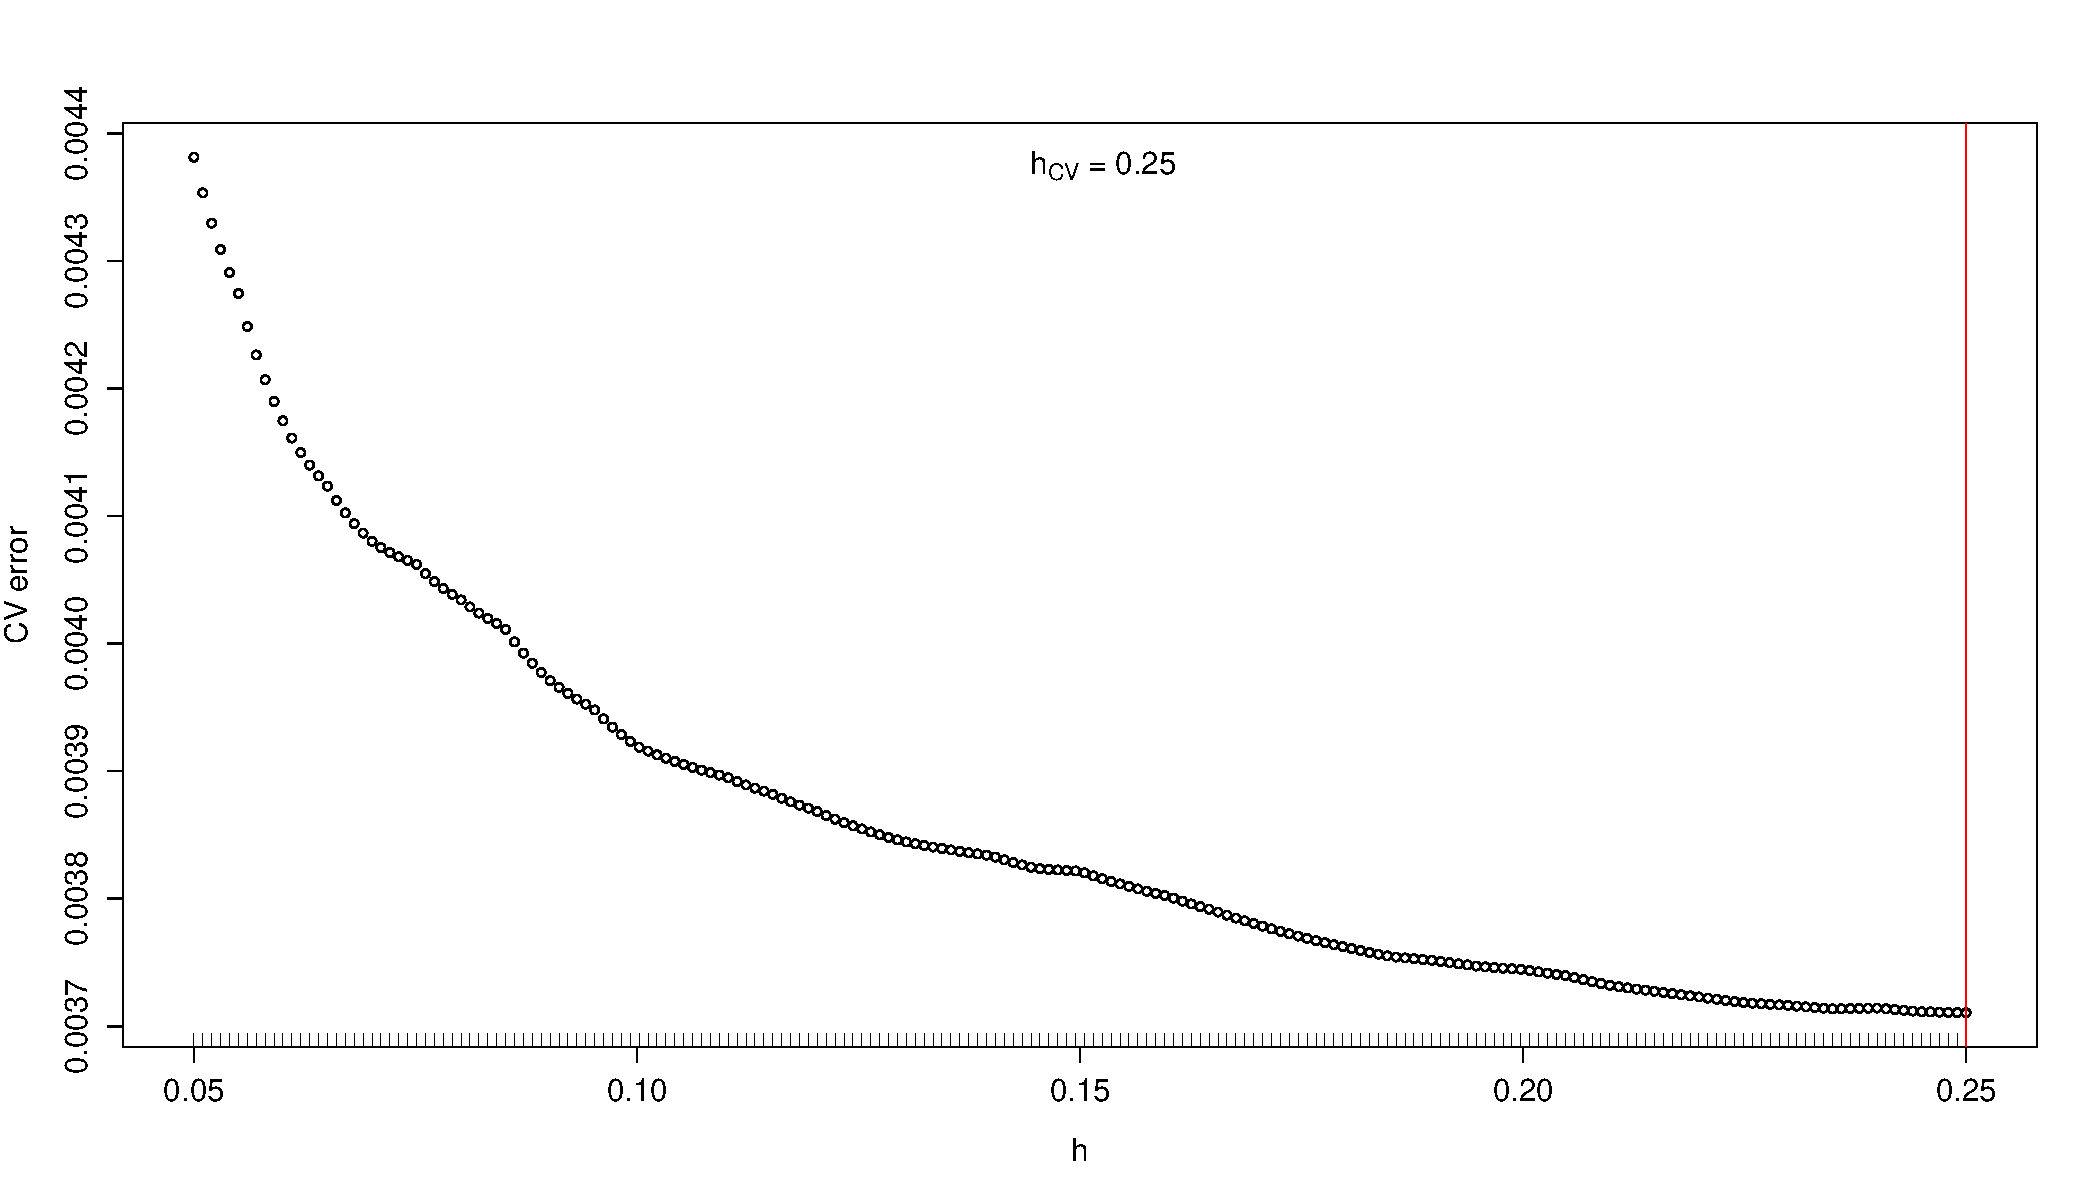
\includegraphics[trim=0 0 20 40, clip, width=\textwidth]{figure_16b.pdf}
		\caption{Local linear estimator}
		\label{fig:application_left_ll}
	\end{subfigure}
	\caption{CV error over a grid of 200 bandwidths for the left side to the threshold in Figure~\ref{fig:application_fits}.
			 The optimal bandwidth is indicated by the red line.}
	\label{fig:application_left}
\end{figure}

\begin{figure}
	\centering
	\begin{subfigure}{0.75\textwidth}
		\centering
		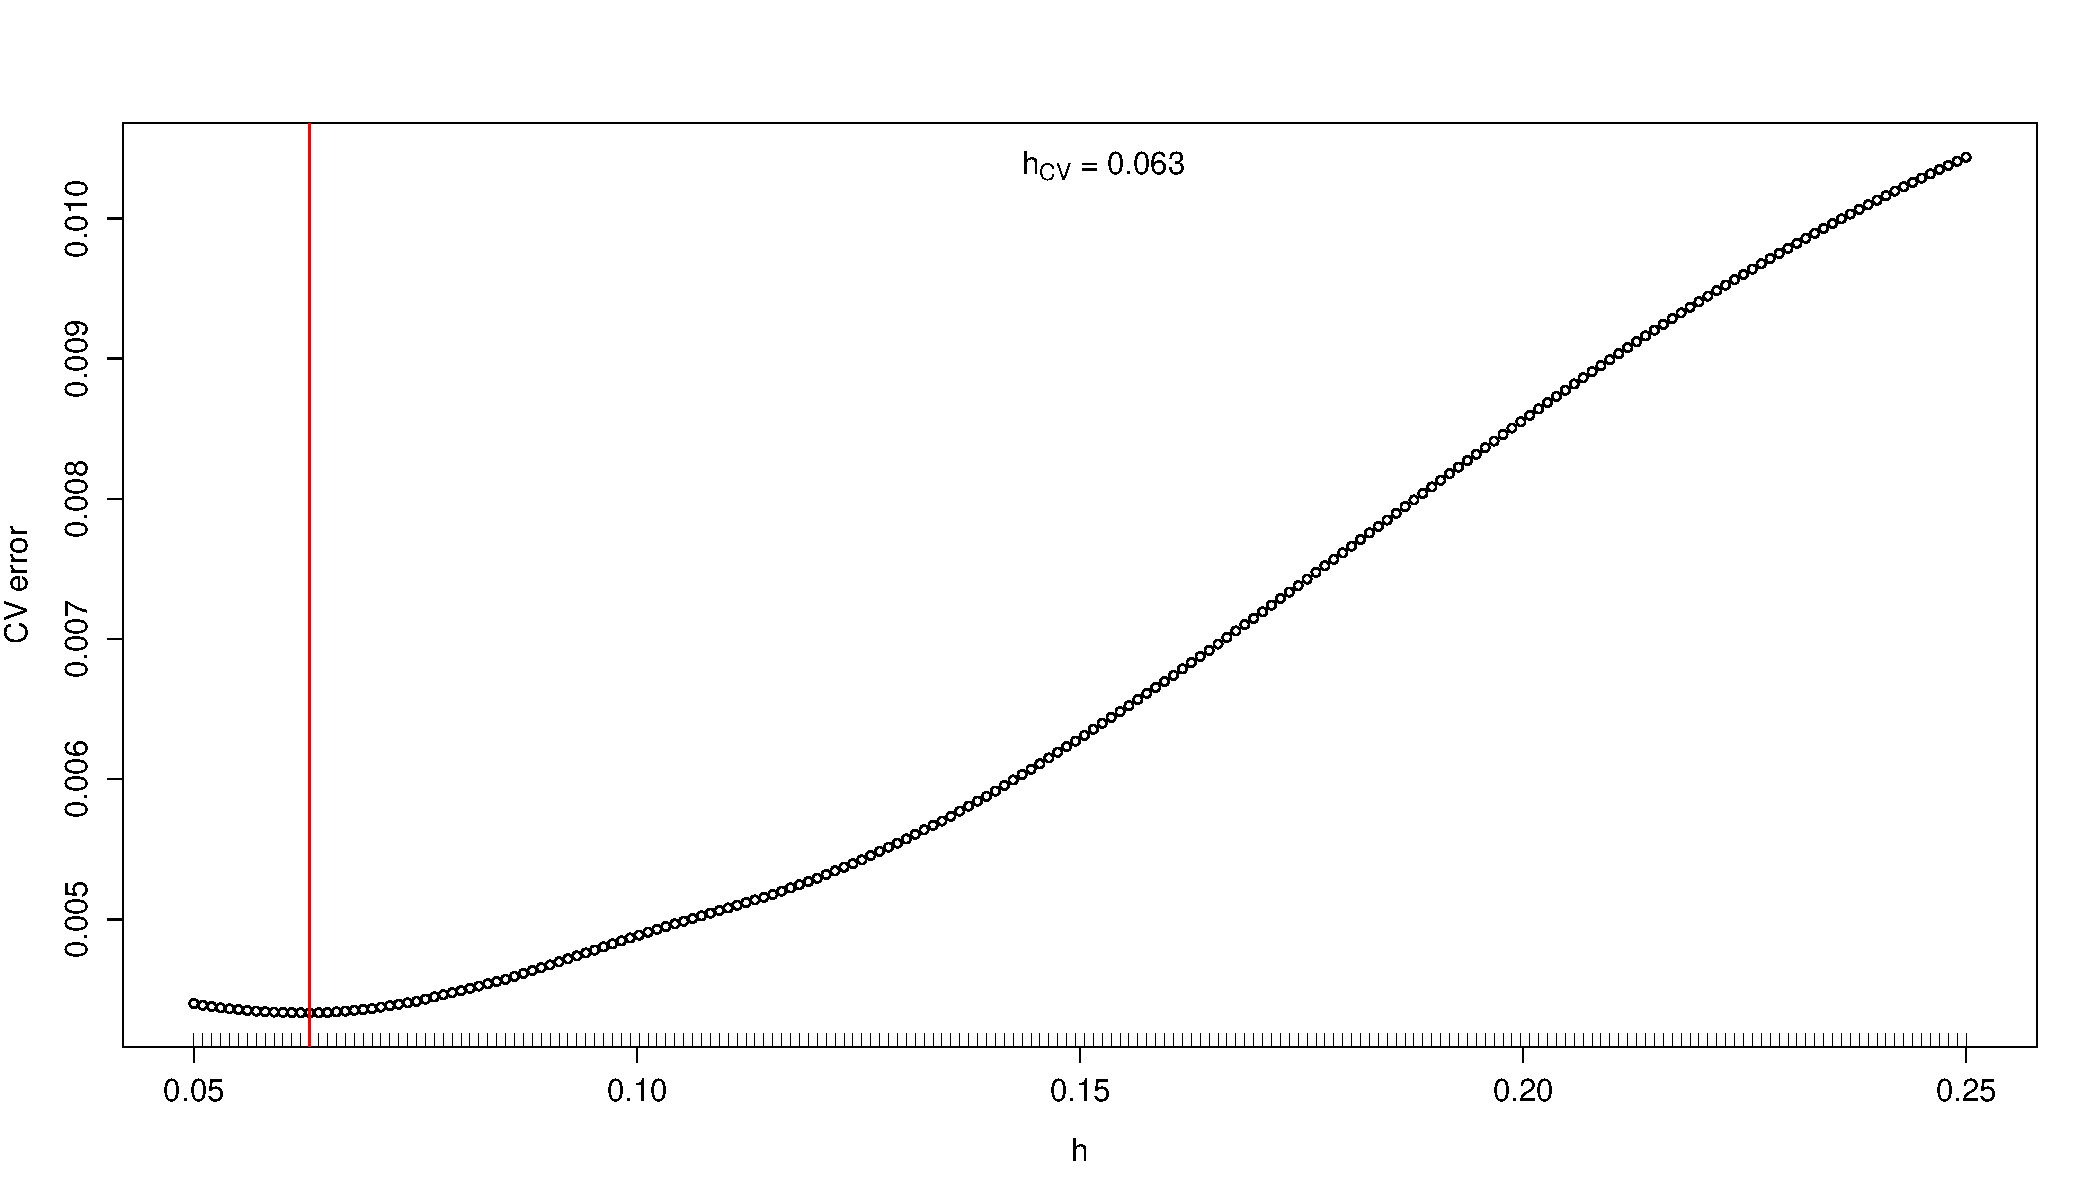
\includegraphics[trim=0 0 20 45, clip, width=\textwidth]{figure_17a.pdf}
		\caption{Nadaraya-Watson estimator}
		\label{fig:application_right_nw}
	\end{subfigure}
	
	\begin{subfigure}{0.75\textwidth}
		\centering
		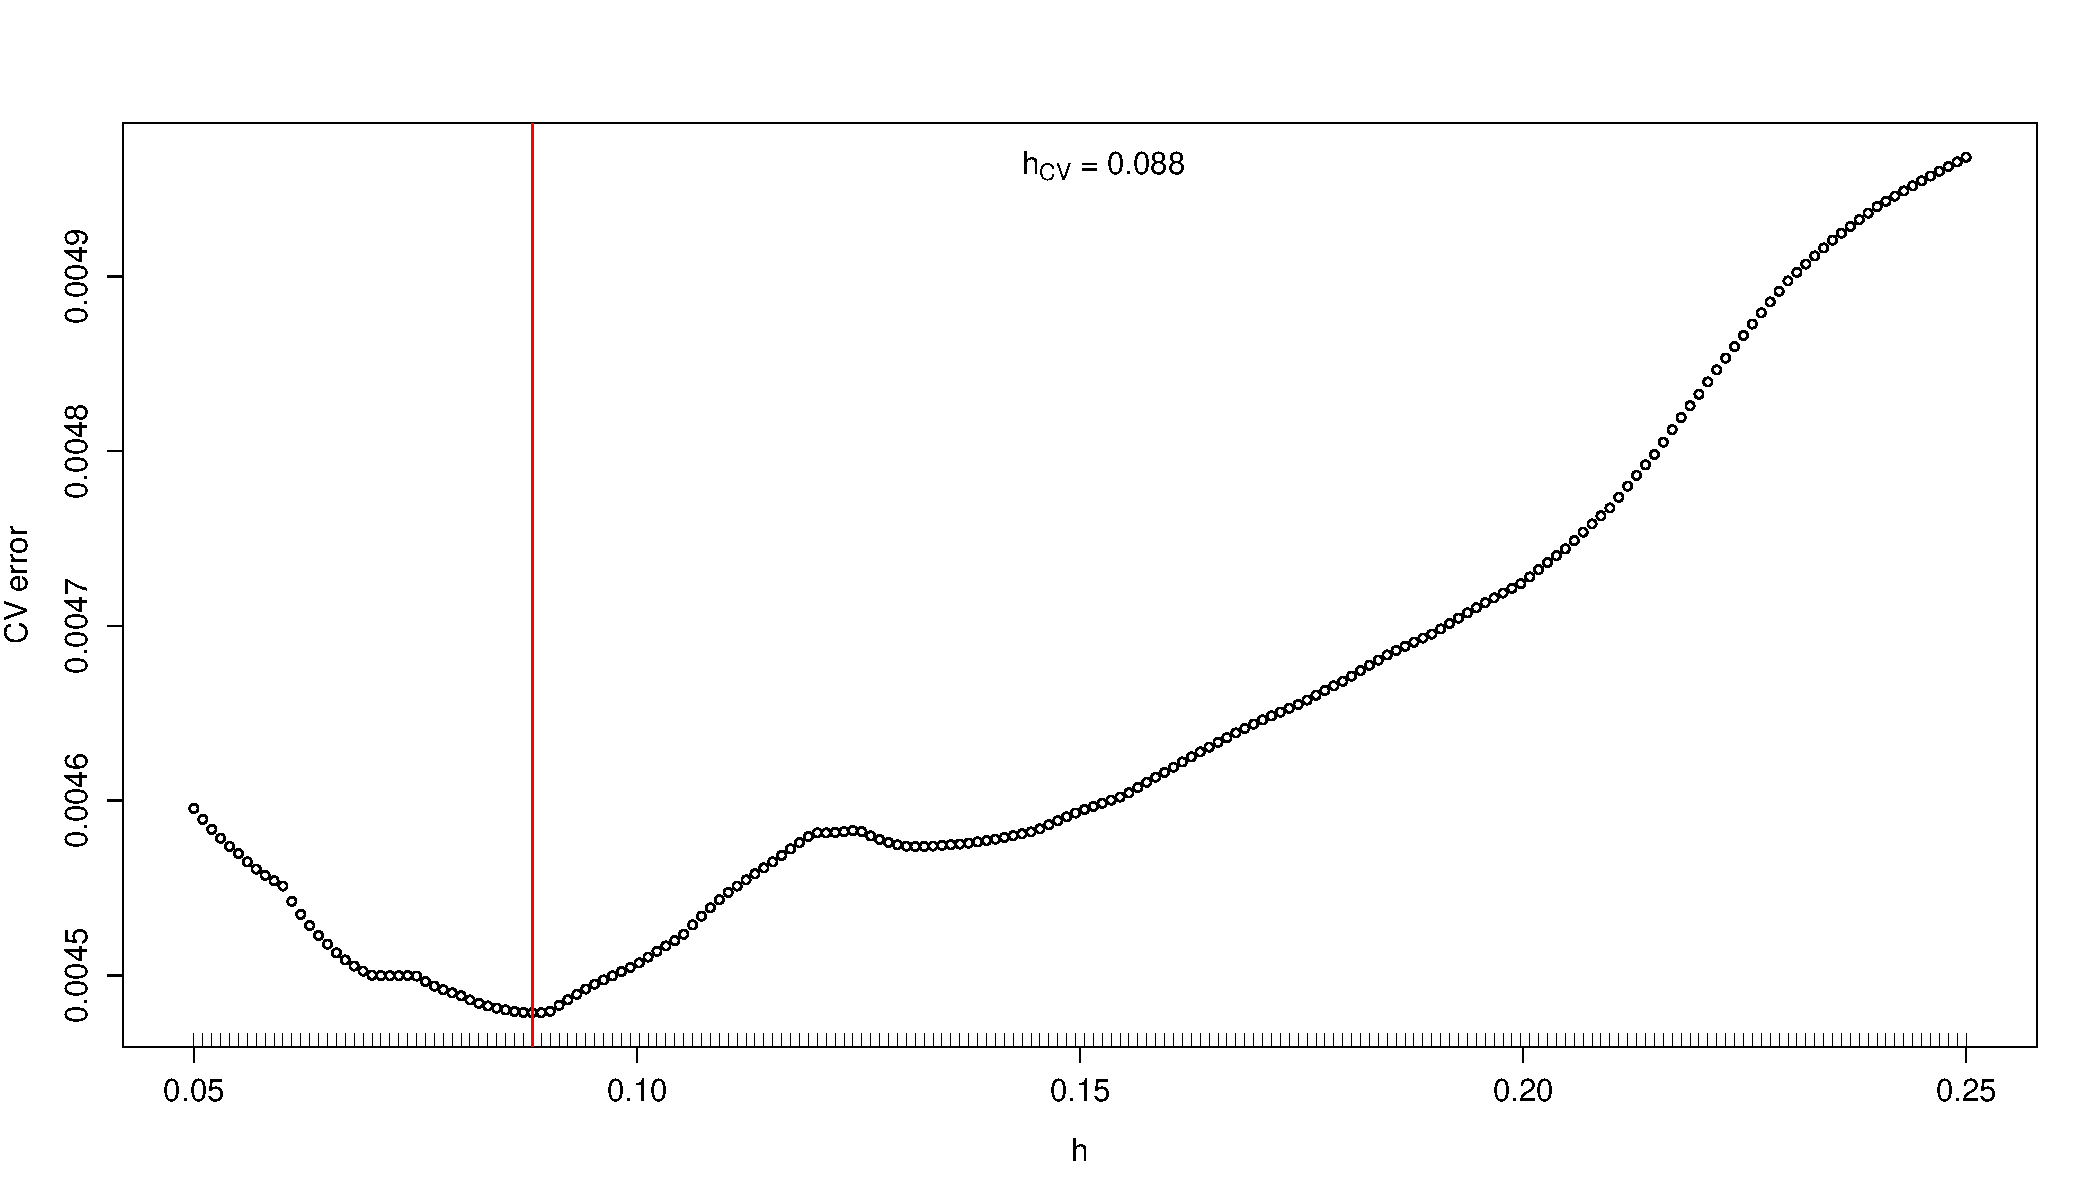
\includegraphics[trim=0 0 20 45, clip, width=\textwidth]{figure_17b.pdf}
		\caption{Local linear estimator}
		\label{fig:application_right_ll}
	\end{subfigure}
	\caption{CV error over a grid of 200 bandwidths for the right side to the threshold in Figure~\ref{fig:application_fits}.
			 The optimal bandwidth is indicated by the red line.}
	\label{fig:application_right}
\end{figure}

\clearpage
 
\printbibliography  

\end{document}